\documentclass[twoside]{book}

% Packages required by doxygen
\usepackage{fixltx2e}
\usepackage{calc}
\usepackage{doxygen}
\usepackage[export]{adjustbox} % also loads graphicx
\usepackage{graphicx}
\usepackage[utf8]{inputenc}
\usepackage{makeidx}
\usepackage{multicol}
\usepackage{multirow}
\PassOptionsToPackage{warn}{textcomp}
\usepackage{textcomp}
\usepackage[nointegrals]{wasysym}
\usepackage[table]{xcolor}

% NLS support packages
\usepackage[spanish]{babel}
% Font selection
\usepackage[T1]{fontenc}
\usepackage[scaled=.90]{helvet}
\usepackage{courier}
\usepackage{amssymb}
\usepackage{sectsty}
\renewcommand{\familydefault}{\sfdefault}
\allsectionsfont{%
  \fontseries{bc}\selectfont%
  \color{darkgray}%
}
\renewcommand{\DoxyLabelFont}{%
  \fontseries{bc}\selectfont%
  \color{darkgray}%
}
\newcommand{\+}{\discretionary{\mbox{\scriptsize$\hookleftarrow$}}{}{}}

% Page & text layout
\usepackage{geometry}
\geometry{%
  a4paper,%
  top=2.5cm,%
  bottom=2.5cm,%
  left=2.5cm,%
  right=2.5cm%
}
\tolerance=750
\hfuzz=15pt
\hbadness=750
\setlength{\emergencystretch}{15pt}
\setlength{\parindent}{0cm}
\setlength{\parskip}{3ex plus 2ex minus 2ex}
\makeatletter
\renewcommand{\paragraph}{%
  \@startsection{paragraph}{4}{0ex}{-1.0ex}{1.0ex}{%
    \normalfont\normalsize\bfseries\SS@parafont%
  }%
}
\renewcommand{\subparagraph}{%
  \@startsection{subparagraph}{5}{0ex}{-1.0ex}{1.0ex}{%
    \normalfont\normalsize\bfseries\SS@subparafont%
  }%
}
\makeatother

% Headers & footers
\usepackage{fancyhdr}
\pagestyle{fancyplain}
\fancyhead[LE]{\fancyplain{}{\bfseries\thepage}}
\fancyhead[CE]{\fancyplain{}{}}
\fancyhead[RE]{\fancyplain{}{\bfseries\leftmark}}
\fancyhead[LO]{\fancyplain{}{\bfseries\rightmark}}
\fancyhead[CO]{\fancyplain{}{}}
\fancyhead[RO]{\fancyplain{}{\bfseries\thepage}}
\fancyfoot[LE]{\fancyplain{}{}}
\fancyfoot[CE]{\fancyplain{}{}}
\fancyfoot[RE]{\fancyplain{}{\bfseries\scriptsize Generado por Doxygen }}
\fancyfoot[LO]{\fancyplain{}{\bfseries\scriptsize Generado por Doxygen }}
\fancyfoot[CO]{\fancyplain{}{}}
\fancyfoot[RO]{\fancyplain{}{}}
\renewcommand{\footrulewidth}{0.4pt}
\renewcommand{\chaptermark}[1]{%
  \markboth{#1}{}%
}
\renewcommand{\sectionmark}[1]{%
  \markright{\thesection\ #1}%
}

% Indices & bibliography
\usepackage{natbib}
\usepackage[titles]{tocloft}
\setcounter{tocdepth}{3}
\setcounter{secnumdepth}{5}
\makeindex

% Hyperlinks (required, but should be loaded last)
\usepackage{ifpdf}
\ifpdf
  \usepackage[pdftex,pagebackref=true]{hyperref}
\else
  \usepackage[ps2pdf,pagebackref=true]{hyperref}
\fi
\hypersetup{%
  colorlinks=true,%
  linkcolor=blue,%
  citecolor=blue,%
  unicode%
}

% Custom commands
\newcommand{\clearemptydoublepage}{%
  \newpage{\pagestyle{empty}\cleardoublepage}%
}

\usepackage{caption}
\captionsetup{labelsep=space,justification=centering,font={bf},singlelinecheck=off,skip=4pt,position=top}

%===== C O N T E N T S =====

\begin{document}

% Titlepage & ToC
\hypersetup{pageanchor=false,
             bookmarksnumbered=true,
             pdfencoding=unicode
            }
\pagenumbering{roman}
\begin{titlepage}
\vspace*{7cm}
\begin{center}%
{\Large Championship \\[1ex]\large 2.\+00 }\\
\vspace*{1cm}
{\large Generado por Doxygen 1.8.11}\\
\end{center}
\end{titlepage}
\clearemptydoublepage
\tableofcontents
\clearemptydoublepage
\pagenumbering{arabic}
\hypersetup{pageanchor=true}

%--- Begin generated contents ---
\chapter{Indice jerárquico}
\section{Jerarquía de la clase}
Esta lista de herencias esta ordenada aproximadamente por orden alfabético\+:\begin{DoxyCompactList}
\item \contentsline{section}{Date}{\pageref{class_date}}{}
\item \contentsline{section}{Participant}{\pageref{class_participant}}{}
\item Q\+Main\+Window\begin{DoxyCompactList}
\item \contentsline{section}{Main\+Window}{\pageref{class_main_window}}{}
\end{DoxyCompactList}
\end{DoxyCompactList}

\chapter{Índice de estructura de datos}
\section{Estructura de datos}
Lista de estructuras con una breve descripción\+:\begin{DoxyCompactList}
\item\contentsline{section}{\hyperlink{class_date}{Date} \\*Clase \hyperlink{class_date}{Date} }{\pageref{class_date}}{}
\item\contentsline{section}{\hyperlink{class_main_window}{Main\+Window} \\*Clase \hyperlink{class_main_window}{Main\+Window} }{\pageref{class_main_window}}{}
\item\contentsline{section}{\hyperlink{class_participant}{Participant} \\*Clase \hyperlink{class_participant}{Participant} }{\pageref{class_participant}}{}
\end{DoxyCompactList}

\chapter{Indice de archivos}
\section{Lista de archivos}
Lista de todos los archivos documentados y con descripciones breves\+:\begin{DoxyCompactList}
\item\contentsline{section}{/home/eduuardoperez/pr3/championship-\/\+P\+R3\+\_\+\+U\+L\+A/project/\hyperlink{date_8cpp}{date.\+cpp} \\*Implementación de la clase \hyperlink{class_date}{Date} }{\pageref{date_8cpp}}{}
\item\contentsline{section}{/home/eduuardoperez/pr3/championship-\/\+P\+R3\+\_\+\+U\+L\+A/project/\hyperlink{date_8h}{date.\+h} \\*Clase \hyperlink{class_date}{Date} }{\pageref{date_8h}}{}
\item\contentsline{section}{/home/eduuardoperez/pr3/championship-\/\+P\+R3\+\_\+\+U\+L\+A/project/\hyperlink{event_8cpp}{event.\+cpp} \\*Implementación de la clase \hyperlink{class_event}{Event} }{\pageref{event_8cpp}}{}
\item\contentsline{section}{/home/eduuardoperez/pr3/championship-\/\+P\+R3\+\_\+\+U\+L\+A/project/\hyperlink{event_8h}{event.\+h} \\*Clase \hyperlink{class_event}{Event} }{\pageref{event_8h}}{}
\item\contentsline{section}{/home/eduuardoperez/pr3/championship-\/\+P\+R3\+\_\+\+U\+L\+A/project/{\bfseries main.\+cpp} }{\pageref{main_8cpp}}{}
\item\contentsline{section}{/home/eduuardoperez/pr3/championship-\/\+P\+R3\+\_\+\+U\+L\+A/project/\hyperlink{mainwindow_8cpp}{mainwindow.\+cpp} \\*Implementación de la clase \hyperlink{class_main_window}{Main\+Window} }{\pageref{mainwindow_8cpp}}{}
\item\contentsline{section}{/home/eduuardoperez/pr3/championship-\/\+P\+R3\+\_\+\+U\+L\+A/project/\hyperlink{mainwindow_8h}{mainwindow.\+h} \\*Clase \hyperlink{class_main_window}{Main\+Window} }{\pageref{mainwindow_8h}}{}
\item\contentsline{section}{/home/eduuardoperez/pr3/championship-\/\+P\+R3\+\_\+\+U\+L\+A/project/\hyperlink{modeventwindow_8cpp}{modeventwindow.\+cpp} \\*Implementación de la clase \hyperlink{class_mod_event_window}{Mod\+Event\+Window} }{\pageref{modeventwindow_8cpp}}{}
\item\contentsline{section}{/home/eduuardoperez/pr3/championship-\/\+P\+R3\+\_\+\+U\+L\+A/project/\hyperlink{modeventwindow_8h}{modeventwindow.\+h} \\*Clase \hyperlink{class_mod_event_window}{Mod\+Event\+Window} }{\pageref{modeventwindow_8h}}{}
\item\contentsline{section}{/home/eduuardoperez/pr3/championship-\/\+P\+R3\+\_\+\+U\+L\+A/project/\hyperlink{organizingwindow_8cpp}{organizingwindow.\+cpp} \\*Implementación de la clase \hyperlink{class_organizing_window}{Organizing\+Window} }{\pageref{organizingwindow_8cpp}}{}
\item\contentsline{section}{/home/eduuardoperez/pr3/championship-\/\+P\+R3\+\_\+\+U\+L\+A/project/\hyperlink{organizingwindow_8h}{organizingwindow.\+h} \\*Clase \hyperlink{class_organizing_window}{Organizing\+Window} }{\pageref{organizingwindow_8h}}{}
\item\contentsline{section}{/home/eduuardoperez/pr3/championship-\/\+P\+R3\+\_\+\+U\+L\+A/project/\hyperlink{participant_8cpp}{participant.\+cpp} \\*Implementación de la clase \hyperlink{class_participant}{Participant} }{\pageref{participant_8cpp}}{}
\item\contentsline{section}{/home/eduuardoperez/pr3/championship-\/\+P\+R3\+\_\+\+U\+L\+A/project/\hyperlink{participant_8h}{participant.\+h} \\*Clase \hyperlink{class_participant}{Participant} }{\pageref{participant_8h}}{}
\item\contentsline{section}{/home/eduuardoperez/pr3/championship-\/\+P\+R3\+\_\+\+U\+L\+A/project/\hyperlink{regeventwindow_8cpp}{regeventwindow.\+cpp} \\*Implementación de la clase \hyperlink{class_reg_event_window}{Reg\+Event\+Window} }{\pageref{regeventwindow_8cpp}}{}
\item\contentsline{section}{/home/eduuardoperez/pr3/championship-\/\+P\+R3\+\_\+\+U\+L\+A/project/\hyperlink{regeventwindow_8h}{regeventwindow.\+h} \\*Clase \hyperlink{class_reg_event_window}{Reg\+Event\+Window} }{\pageref{regeventwindow_8h}}{}
\item\contentsline{section}{/home/eduuardoperez/pr3/championship-\/\+P\+R3\+\_\+\+U\+L\+A/project/\hyperlink{sportywindow_8cpp}{sportywindow.\+cpp} \\*Implementación de la clase \hyperlink{class_sporty_window}{Sporty\+Window} }{\pageref{sportywindow_8cpp}}{}
\item\contentsline{section}{/home/eduuardoperez/pr3/championship-\/\+P\+R3\+\_\+\+U\+L\+A/project/\hyperlink{sportywindow_8h}{sportywindow.\+h} \\*Clase \hyperlink{class_sporty_window}{Sporty\+Window} }{\pageref{sportywindow_8h}}{}
\item\contentsline{section}{/home/eduuardoperez/pr3/championship-\/\+P\+R3\+\_\+\+U\+L\+A/project/{\bfseries viewevent.\+cpp} }{\pageref{viewevent_8cpp}}{}
\item\contentsline{section}{/home/eduuardoperez/pr3/championship-\/\+P\+R3\+\_\+\+U\+L\+A/project/{\bfseries viewevent.\+h} }{\pageref{viewevent_8h}}{}
\end{DoxyCompactList}

\chapter{Documentación de las estructuras de datos}
\hypertarget{class_date}{}\section{Referencia de la Clase Date}
\label{class_date}\index{Date@{Date}}


Clase \hyperlink{class_date}{Date}.  




{\ttfamily \#include $<$date.\+h$>$}

\subsection*{Métodos públicos}
\begin{DoxyCompactItemize}
\item 
\hyperlink{class_date_afa65693475fb86a2de04c8578b232201}{Date} (const \hyperlink{class_date}{Date} \&)\hypertarget{class_date_afa65693475fb86a2de04c8578b232201}{}\label{class_date_afa65693475fb86a2de04c8578b232201}

\begin{DoxyCompactList}\small\item\em Constructor por copia de la clase \hyperlink{class_date}{Date}. \end{DoxyCompactList}\item 
unsigned int \hyperlink{class_date_a254204c492d3ebc26a2c62d532e34844}{get\+Day} () const 
\begin{DoxyCompactList}\small\item\em Observador get\+Day. \end{DoxyCompactList}\item 
unsigned int \hyperlink{class_date_ac471b901531b7a1e73809918bac8c1ec}{get\+Month} () const 
\begin{DoxyCompactList}\small\item\em Observador get\+Month. \end{DoxyCompactList}\item 
unsigned int \hyperlink{class_date_a6561cf495bd6b7e6c747420d7ae9cc12}{get\+Year} () const 
\begin{DoxyCompactList}\small\item\em Observador get\+Year. \end{DoxyCompactList}\item 
void \hyperlink{class_date_aafe200d5fe2aa294a91d20a6b97afe75}{set\+Day} (unsigned int)\hypertarget{class_date_aafe200d5fe2aa294a91d20a6b97afe75}{}\label{class_date_aafe200d5fe2aa294a91d20a6b97afe75}

\begin{DoxyCompactList}\small\item\em Modificador set\+Day. \end{DoxyCompactList}\item 
void \hyperlink{class_date_aae2c1d1158d2760ba4d5a23c528fd24d}{set\+Month} (unsigned int)\hypertarget{class_date_aae2c1d1158d2760ba4d5a23c528fd24d}{}\label{class_date_aae2c1d1158d2760ba4d5a23c528fd24d}

\begin{DoxyCompactList}\small\item\em Modificador set\+Month. \end{DoxyCompactList}\item 
void \hyperlink{class_date_abf7cafce8365f4ad601c270bb3f0f02d}{set\+Year} (unsigned int)\hypertarget{class_date_abf7cafce8365f4ad601c270bb3f0f02d}{}\label{class_date_abf7cafce8365f4ad601c270bb3f0f02d}

\begin{DoxyCompactList}\small\item\em Modificador set\+Year. \end{DoxyCompactList}\item 
void \hyperlink{class_date_a4ca1e1caba11928c842f6c62a2c851ab}{from\+String} (string)\hypertarget{class_date_a4ca1e1caba11928c842f6c62a2c851ab}{}\label{class_date_a4ca1e1caba11928c842f6c62a2c851ab}

\begin{DoxyCompactList}\small\item\em Método from\+String. \end{DoxyCompactList}\item 
string \hyperlink{class_date_adebdb45904dc2fbfacc66aa7528e0c04}{to\+String} ()
\begin{DoxyCompactList}\small\item\em Método to\+String. \end{DoxyCompactList}\item 
int \hyperlink{class_date_ae8b8f304223099e3ecf37e64232c757a}{cmp\+Date} (\hyperlink{class_date}{Date})
\begin{DoxyCompactList}\small\item\em Método cmp\+Date. \end{DoxyCompactList}\item 
void \hyperlink{class_date_a2ad9e0b62b3abea9c9d471373ce5fdef}{assign} (unsigned int, unsigned int, unsigned int)\hypertarget{class_date_a2ad9e0b62b3abea9c9d471373ce5fdef}{}\label{class_date_a2ad9e0b62b3abea9c9d471373ce5fdef}

\begin{DoxyCompactList}\small\item\em Método assign. \end{DoxyCompactList}\item 
\hyperlink{class_date}{Date} \hyperlink{class_date_a449df9445b4f4fac127e171ac981adb3}{operator=} (const \hyperlink{class_date}{Date} \&)
\begin{DoxyCompactList}\small\item\em operator = \end{DoxyCompactList}\item 
int \hyperlink{class_date_aea7500eb1bee5e573c01c32458bbe83e}{operator==} (const \hyperlink{class_date}{Date} \&)
\begin{DoxyCompactList}\small\item\em operator == \end{DoxyCompactList}\end{DoxyCompactItemize}


\subsection{Descripción detallada}
Clase \hyperlink{class_date}{Date}. 

Definición en la línea 21 del archivo date.\+h.



\subsection{Documentación de las funciones miembro}
\index{Date@{Date}!cmp\+Date@{cmp\+Date}}
\index{cmp\+Date@{cmp\+Date}!Date@{Date}}
\subsubsection[{\texorpdfstring{cmp\+Date(\+Date)}{cmpDate(Date)}}]{\setlength{\rightskip}{0pt plus 5cm}int Date\+::cmp\+Date (
\begin{DoxyParamCaption}
\item[{{\bf Date}}]{date}
\end{DoxyParamCaption}
)}\hypertarget{class_date_ae8b8f304223099e3ecf37e64232c757a}{}\label{class_date_ae8b8f304223099e3ecf37e64232c757a}


Método cmp\+Date. 

\begin{DoxyReturn}{Devuelve}
entero negativo si this es menor que date, 0 si this es igual a date, entero positivo si this es mayor que date. 
\end{DoxyReturn}


Definición en la línea 73 del archivo date.\+cpp.

\index{Date@{Date}!get\+Day@{get\+Day}}
\index{get\+Day@{get\+Day}!Date@{Date}}
\subsubsection[{\texorpdfstring{get\+Day() const }{getDay() const }}]{\setlength{\rightskip}{0pt plus 5cm}unsigned int Date\+::get\+Day (
\begin{DoxyParamCaption}
{}
\end{DoxyParamCaption}
) const\hspace{0.3cm}{\ttfamily [inline]}}\hypertarget{class_date_a254204c492d3ebc26a2c62d532e34844}{}\label{class_date_a254204c492d3ebc26a2c62d532e34844}


Observador get\+Day. 

\begin{DoxyReturn}{Devuelve}
this-\/$>$day 
\end{DoxyReturn}


Definición en la línea 42 del archivo date.\+h.

\index{Date@{Date}!get\+Month@{get\+Month}}
\index{get\+Month@{get\+Month}!Date@{Date}}
\subsubsection[{\texorpdfstring{get\+Month() const }{getMonth() const }}]{\setlength{\rightskip}{0pt plus 5cm}unsigned int Date\+::get\+Month (
\begin{DoxyParamCaption}
{}
\end{DoxyParamCaption}
) const\hspace{0.3cm}{\ttfamily [inline]}}\hypertarget{class_date_ac471b901531b7a1e73809918bac8c1ec}{}\label{class_date_ac471b901531b7a1e73809918bac8c1ec}


Observador get\+Month. 

\begin{DoxyReturn}{Devuelve}
this-\/$>$month 
\end{DoxyReturn}


Definición en la línea 51 del archivo date.\+h.

\index{Date@{Date}!get\+Year@{get\+Year}}
\index{get\+Year@{get\+Year}!Date@{Date}}
\subsubsection[{\texorpdfstring{get\+Year() const }{getYear() const }}]{\setlength{\rightskip}{0pt plus 5cm}unsigned int Date\+::get\+Year (
\begin{DoxyParamCaption}
{}
\end{DoxyParamCaption}
) const\hspace{0.3cm}{\ttfamily [inline]}}\hypertarget{class_date_a6561cf495bd6b7e6c747420d7ae9cc12}{}\label{class_date_a6561cf495bd6b7e6c747420d7ae9cc12}


Observador get\+Year. 

\begin{DoxyReturn}{Devuelve}
this-\/$>$year 
\end{DoxyReturn}


Definición en la línea 60 del archivo date.\+h.

\index{Date@{Date}!operator=@{operator=}}
\index{operator=@{operator=}!Date@{Date}}
\subsubsection[{\texorpdfstring{operator=(const Date \&)}{operator=(const Date &)}}]{\setlength{\rightskip}{0pt plus 5cm}{\bf Date} Date\+::operator= (
\begin{DoxyParamCaption}
\item[{const {\bf Date} \&}]{date}
\end{DoxyParamCaption}
)}\hypertarget{class_date_a449df9445b4f4fac127e171ac981adb3}{}\label{class_date_a449df9445b4f4fac127e171ac981adb3}


operator = 

\begin{DoxyReturn}{Devuelve}
\hyperlink{class_date}{Date} date 
\end{DoxyReturn}


Definición en la línea 93 del archivo date.\+cpp.

\index{Date@{Date}!operator==@{operator==}}
\index{operator==@{operator==}!Date@{Date}}
\subsubsection[{\texorpdfstring{operator==(const Date \&)}{operator==(const Date &)}}]{\setlength{\rightskip}{0pt plus 5cm}int Date\+::operator== (
\begin{DoxyParamCaption}
\item[{const {\bf Date} \&}]{date}
\end{DoxyParamCaption}
)}\hypertarget{class_date_aea7500eb1bee5e573c01c32458bbe83e}{}\label{class_date_aea7500eb1bee5e573c01c32458bbe83e}


operator == 

\begin{DoxyReturn}{Devuelve}
1 si this es igual a date, 0 si no lo es. 
\end{DoxyReturn}


Definición en la línea 101 del archivo date.\+cpp.

\index{Date@{Date}!to\+String@{to\+String}}
\index{to\+String@{to\+String}!Date@{Date}}
\subsubsection[{\texorpdfstring{to\+String()}{toString()}}]{\setlength{\rightskip}{0pt plus 5cm}string Date\+::to\+String (
\begin{DoxyParamCaption}
{}
\end{DoxyParamCaption}
)}\hypertarget{class_date_adebdb45904dc2fbfacc66aa7528e0c04}{}\label{class_date_adebdb45904dc2fbfacc66aa7528e0c04}


Método to\+String. 

\begin{DoxyReturn}{Devuelve}
tipo \hyperlink{class_date}{Date} convertido a string 
\end{DoxyReturn}


Definición en la línea 65 del archivo date.\+cpp.



La documentación para esta clase fue generada a partir de los siguientes ficheros\+:\begin{DoxyCompactItemize}
\item 
/home/eduuardoperez/pr3/championship/project/\hyperlink{date_8h}{date.\+h}\item 
/home/eduuardoperez/pr3/championship/project/\hyperlink{date_8cpp}{date.\+cpp}\end{DoxyCompactItemize}

\hypertarget{class_event}{}\section{Referencia de la Clase Event}
\label{class_event}\index{Event@{Event}}


Clase \hyperlink{class_event}{Event}.  




{\ttfamily \#include $<$event.\+h$>$}

\subsection*{Métodos públicos}
\begin{DoxyCompactItemize}
\item 
\hyperlink{class_event_ac540d5e149dc8f0670ce49d1a1bc4d98}{Event} (const \hyperlink{class_event}{Event} \&)\hypertarget{class_event_ac540d5e149dc8f0670ce49d1a1bc4d98}{}\label{class_event_ac540d5e149dc8f0670ce49d1a1bc4d98}

\begin{DoxyCompactList}\small\item\em Constructor por copia de la clase \hyperlink{class_event}{Event}. \end{DoxyCompactList}\item 
string \hyperlink{class_event_a039da9c8718a10118c751cfece9c0202}{get\+Event\+Name} () const 
\begin{DoxyCompactList}\small\item\em Observador get\+Event\+Name. \end{DoxyCompactList}\item 
\hyperlink{class_date}{Date} \hyperlink{class_event_a02a80e4f88bb11f0f13b2c4d77e14608}{get\+Date\+Beg\+Ev} () const 
\begin{DoxyCompactList}\small\item\em Observador get\+Date\+Beg\+Ev. \end{DoxyCompactList}\item 
\hyperlink{class_date}{Date} \hyperlink{class_event_ad08ca642b7b5fcc7884673169e60e10a}{get\+Date\+Fin\+Ev} () const 
\begin{DoxyCompactList}\small\item\em Observador get\+Date\+Fin\+Ev. \end{DoxyCompactList}\item 
float \hyperlink{class_event_a38ceadf6f0b9c60d4c4040c09123fb90}{get\+Inscrip\+Value} () const 
\begin{DoxyCompactList}\small\item\em Observador get\+Inscrip\+Value. \end{DoxyCompactList}\item 
string \hyperlink{class_event_a972bab2aa104037272cf41eddb96b8af}{get\+Event\+Hour} () const 
\begin{DoxyCompactList}\small\item\em Observador get\+Event\+Hour. \end{DoxyCompactList}\item 
string \hyperlink{class_event_aa74ed15321f27ab38bd883271433b9dd}{get\+Event\+Place} () const 
\begin{DoxyCompactList}\small\item\em Observador get\+Event\+Place. \end{DoxyCompactList}\item 
\hyperlink{class_date}{Date} \hyperlink{class_event_a0466f9ab15328e36f6d117280f570544}{get\+Date\+Beg\+Mate} () const 
\begin{DoxyCompactList}\small\item\em Observador get\+Date\+Beg\+Mate. \end{DoxyCompactList}\item 
\hyperlink{class_date}{Date} \hyperlink{class_event_a8676a4856cdb6e84f78ca1fa9988b2ca}{get\+Date\+Fin\+Mate} () const 
\begin{DoxyCompactList}\small\item\em Observador get\+Date\+Fin\+Mate. \end{DoxyCompactList}\item 
string \hyperlink{class_event_a7bd9666f47f9dceaca300482653778de}{get\+Hour\+Ini\+Mate} () const 
\begin{DoxyCompactList}\small\item\em Observador get\+Hour\+Ini\+Mate. \end{DoxyCompactList}\item 
string \hyperlink{class_event_ab0b79d0fde419c36eeddce0974aa29b0}{get\+Hour\+Fin\+Mate} () const 
\begin{DoxyCompactList}\small\item\em Observador get\+Hour\+Fin\+Mate. \end{DoxyCompactList}\item 
string \hyperlink{class_event_a8dfff443f2f78fd86705afe00b8e0489}{get\+Mate\+Place} () const 
\begin{DoxyCompactList}\small\item\em Observador get\+Mate\+Place. \end{DoxyCompactList}\item 
string \hyperlink{class_event_aaaf95f81e1f746ef936bacb569306b05}{get\+Description} () const 
\begin{DoxyCompactList}\small\item\em Observador get\+Description. \end{DoxyCompactList}\item 
string \hyperlink{class_event_aa85b8f3c2d3f220e87b80396767fc746}{get\+Picture} () const 
\begin{DoxyCompactList}\small\item\em Observador get\+Picture. \end{DoxyCompactList}\item 
void \hyperlink{class_event_aa72ec9ac1dc30b3afdf8a0da60d92e31}{set\+Event\+Name} (string)\hypertarget{class_event_aa72ec9ac1dc30b3afdf8a0da60d92e31}{}\label{class_event_aa72ec9ac1dc30b3afdf8a0da60d92e31}

\begin{DoxyCompactList}\small\item\em Modificador set\+Event\+Name. \end{DoxyCompactList}\item 
void \hyperlink{class_event_ac8d69d760bad23c2aefea2c5b48cb8f8}{set\+Date\+Beg\+Ev} (\hyperlink{class_date}{Date})\hypertarget{class_event_ac8d69d760bad23c2aefea2c5b48cb8f8}{}\label{class_event_ac8d69d760bad23c2aefea2c5b48cb8f8}

\begin{DoxyCompactList}\small\item\em Modificador set\+Date\+Beg\+Ev. \end{DoxyCompactList}\item 
void \hyperlink{class_event_aec7119f73d4b29560476d9a2d2550992}{set\+Date\+Fin\+Ev} (\hyperlink{class_date}{Date})\hypertarget{class_event_aec7119f73d4b29560476d9a2d2550992}{}\label{class_event_aec7119f73d4b29560476d9a2d2550992}

\begin{DoxyCompactList}\small\item\em Modificador set\+Date\+Fin\+Ev. \end{DoxyCompactList}\item 
void \hyperlink{class_event_acf286ffb8186b161f9fc4833884c5f98}{set\+Inscrip\+Value} (float)\hypertarget{class_event_acf286ffb8186b161f9fc4833884c5f98}{}\label{class_event_acf286ffb8186b161f9fc4833884c5f98}

\begin{DoxyCompactList}\small\item\em Modificador set\+Inscrip\+Value. \end{DoxyCompactList}\item 
void \hyperlink{class_event_a79f9395703795827cbd264612695e73a}{set\+Event\+Hour} (string)\hypertarget{class_event_a79f9395703795827cbd264612695e73a}{}\label{class_event_a79f9395703795827cbd264612695e73a}

\begin{DoxyCompactList}\small\item\em Modificador set\+Event\+Hour. \end{DoxyCompactList}\item 
void \hyperlink{class_event_a7c7f3267118fbd613738b415465dbcac}{set\+Event\+Place} (string)\hypertarget{class_event_a7c7f3267118fbd613738b415465dbcac}{}\label{class_event_a7c7f3267118fbd613738b415465dbcac}

\begin{DoxyCompactList}\small\item\em Modificador set\+Event\+Place. \end{DoxyCompactList}\item 
void \hyperlink{class_event_a9db054102d874e7af959143dcc3c9077}{set\+Date\+Beg\+Mate} (\hyperlink{class_date}{Date})\hypertarget{class_event_a9db054102d874e7af959143dcc3c9077}{}\label{class_event_a9db054102d874e7af959143dcc3c9077}

\begin{DoxyCompactList}\small\item\em Modificador set\+Date\+Beg\+Mate. \end{DoxyCompactList}\item 
void \hyperlink{class_event_aa99f913f889b15275e3da60b014e0283}{set\+Date\+Fin\+Mate} (\hyperlink{class_date}{Date})\hypertarget{class_event_aa99f913f889b15275e3da60b014e0283}{}\label{class_event_aa99f913f889b15275e3da60b014e0283}

\begin{DoxyCompactList}\small\item\em Modificador set\+Date\+Fin\+Mate. \end{DoxyCompactList}\item 
void \hyperlink{class_event_afcfecbce4f34e3bbc8c5b9b1143015f5}{set\+Hour\+Ini\+Mate} (string)\hypertarget{class_event_afcfecbce4f34e3bbc8c5b9b1143015f5}{}\label{class_event_afcfecbce4f34e3bbc8c5b9b1143015f5}

\begin{DoxyCompactList}\small\item\em Modificador set\+Hour\+Ini\+Mate. \end{DoxyCompactList}\item 
void \hyperlink{class_event_ad7e81513dcb7b9fddb7f670171b0402c}{set\+Hour\+Fin\+Mate} (string)\hypertarget{class_event_ad7e81513dcb7b9fddb7f670171b0402c}{}\label{class_event_ad7e81513dcb7b9fddb7f670171b0402c}

\begin{DoxyCompactList}\small\item\em Modificador set\+Hour\+Fin\+Mate. \end{DoxyCompactList}\item 
void \hyperlink{class_event_ac2df54c72bf6a913ef8cea23f9164561}{set\+Mate\+Place} (string)\hypertarget{class_event_ac2df54c72bf6a913ef8cea23f9164561}{}\label{class_event_ac2df54c72bf6a913ef8cea23f9164561}

\begin{DoxyCompactList}\small\item\em Modificador set\+Mate\+Place. \end{DoxyCompactList}\item 
void \hyperlink{class_event_a10101412d581dc0a23e6bde775e8330b}{set\+Description} (string)\hypertarget{class_event_a10101412d581dc0a23e6bde775e8330b}{}\label{class_event_a10101412d581dc0a23e6bde775e8330b}

\begin{DoxyCompactList}\small\item\em Modificador set\+Description. \end{DoxyCompactList}\item 
void \hyperlink{class_event_a6ebd602ac071857bc3603713f372af16}{set\+Picture} (string)\hypertarget{class_event_a6ebd602ac071857bc3603713f372af16}{}\label{class_event_a6ebd602ac071857bc3603713f372af16}

\begin{DoxyCompactList}\small\item\em Modificador set\+Picture. \end{DoxyCompactList}\item 
void \hyperlink{class_event_ad2eac077832eb8afa3f03a9eeb885d52}{assign} (string, \hyperlink{class_date}{Date}, \hyperlink{class_date}{Date}, float, string, string, \hyperlink{class_date}{Date}, \hyperlink{class_date}{Date}, string, string, string, string)\hypertarget{class_event_ad2eac077832eb8afa3f03a9eeb885d52}{}\label{class_event_ad2eac077832eb8afa3f03a9eeb885d52}

\begin{DoxyCompactList}\small\item\em Método assign. \end{DoxyCompactList}\item 
\hyperlink{class_event}{Event} \hyperlink{class_event_aa1f38079195c338a7628867d56cf9196}{operator=} (const \hyperlink{class_event}{Event} \&)
\begin{DoxyCompactList}\small\item\em operator = \end{DoxyCompactList}\item 
int \hyperlink{class_event_aed3bcbc97adc5d34e8f693deb1f99371}{operator==} (const \hyperlink{class_event}{Event} \&)
\begin{DoxyCompactList}\small\item\em operator == \end{DoxyCompactList}\end{DoxyCompactItemize}


\subsection{Descripción detallada}
Clase \hyperlink{class_event}{Event}. 

Definición en la línea 17 del archivo event.\+h.



\subsection{Documentación de las funciones miembro}
\index{Event@{Event}!get\+Date\+Beg\+Ev@{get\+Date\+Beg\+Ev}}
\index{get\+Date\+Beg\+Ev@{get\+Date\+Beg\+Ev}!Event@{Event}}
\subsubsection[{\texorpdfstring{get\+Date\+Beg\+Ev() const }{getDateBegEv() const }}]{\setlength{\rightskip}{0pt plus 5cm}{\bf Date} Event\+::get\+Date\+Beg\+Ev (
\begin{DoxyParamCaption}
{}
\end{DoxyParamCaption}
) const\hspace{0.3cm}{\ttfamily [inline]}}\hypertarget{class_event_a02a80e4f88bb11f0f13b2c4d77e14608}{}\label{class_event_a02a80e4f88bb11f0f13b2c4d77e14608}


Observador get\+Date\+Beg\+Ev. 

\begin{DoxyReturn}{Devuelve}
fecha inicio de this 
\end{DoxyReturn}


Definición en la línea 54 del archivo event.\+h.

\index{Event@{Event}!get\+Date\+Beg\+Mate@{get\+Date\+Beg\+Mate}}
\index{get\+Date\+Beg\+Mate@{get\+Date\+Beg\+Mate}!Event@{Event}}
\subsubsection[{\texorpdfstring{get\+Date\+Beg\+Mate() const }{getDateBegMate() const }}]{\setlength{\rightskip}{0pt plus 5cm}{\bf Date} Event\+::get\+Date\+Beg\+Mate (
\begin{DoxyParamCaption}
{}
\end{DoxyParamCaption}
) const\hspace{0.3cm}{\ttfamily [inline]}}\hypertarget{class_event_a0466f9ab15328e36f6d117280f570544}{}\label{class_event_a0466f9ab15328e36f6d117280f570544}


Observador get\+Date\+Beg\+Mate. 

\begin{DoxyReturn}{Devuelve}
fecha inicio entrega del material para this 
\end{DoxyReturn}


Definición en la línea 99 del archivo event.\+h.

\index{Event@{Event}!get\+Date\+Fin\+Ev@{get\+Date\+Fin\+Ev}}
\index{get\+Date\+Fin\+Ev@{get\+Date\+Fin\+Ev}!Event@{Event}}
\subsubsection[{\texorpdfstring{get\+Date\+Fin\+Ev() const }{getDateFinEv() const }}]{\setlength{\rightskip}{0pt plus 5cm}{\bf Date} Event\+::get\+Date\+Fin\+Ev (
\begin{DoxyParamCaption}
{}
\end{DoxyParamCaption}
) const\hspace{0.3cm}{\ttfamily [inline]}}\hypertarget{class_event_ad08ca642b7b5fcc7884673169e60e10a}{}\label{class_event_ad08ca642b7b5fcc7884673169e60e10a}


Observador get\+Date\+Fin\+Ev. 

\begin{DoxyReturn}{Devuelve}
fecha fin de this 
\end{DoxyReturn}


Definición en la línea 63 del archivo event.\+h.

\index{Event@{Event}!get\+Date\+Fin\+Mate@{get\+Date\+Fin\+Mate}}
\index{get\+Date\+Fin\+Mate@{get\+Date\+Fin\+Mate}!Event@{Event}}
\subsubsection[{\texorpdfstring{get\+Date\+Fin\+Mate() const }{getDateFinMate() const }}]{\setlength{\rightskip}{0pt plus 5cm}{\bf Date} Event\+::get\+Date\+Fin\+Mate (
\begin{DoxyParamCaption}
{}
\end{DoxyParamCaption}
) const\hspace{0.3cm}{\ttfamily [inline]}}\hypertarget{class_event_a8676a4856cdb6e84f78ca1fa9988b2ca}{}\label{class_event_a8676a4856cdb6e84f78ca1fa9988b2ca}


Observador get\+Date\+Fin\+Mate. 

\begin{DoxyReturn}{Devuelve}
fecha fin entrega del material para this 
\end{DoxyReturn}


Definición en la línea 108 del archivo event.\+h.

\index{Event@{Event}!get\+Description@{get\+Description}}
\index{get\+Description@{get\+Description}!Event@{Event}}
\subsubsection[{\texorpdfstring{get\+Description() const }{getDescription() const }}]{\setlength{\rightskip}{0pt plus 5cm}string Event\+::get\+Description (
\begin{DoxyParamCaption}
{}
\end{DoxyParamCaption}
) const\hspace{0.3cm}{\ttfamily [inline]}}\hypertarget{class_event_aaaf95f81e1f746ef936bacb569306b05}{}\label{class_event_aaaf95f81e1f746ef936bacb569306b05}


Observador get\+Description. 

\begin{DoxyReturn}{Devuelve}
descripción de this 
\end{DoxyReturn}


Definición en la línea 144 del archivo event.\+h.

\index{Event@{Event}!get\+Event\+Hour@{get\+Event\+Hour}}
\index{get\+Event\+Hour@{get\+Event\+Hour}!Event@{Event}}
\subsubsection[{\texorpdfstring{get\+Event\+Hour() const }{getEventHour() const }}]{\setlength{\rightskip}{0pt plus 5cm}string Event\+::get\+Event\+Hour (
\begin{DoxyParamCaption}
{}
\end{DoxyParamCaption}
) const\hspace{0.3cm}{\ttfamily [inline]}}\hypertarget{class_event_a972bab2aa104037272cf41eddb96b8af}{}\label{class_event_a972bab2aa104037272cf41eddb96b8af}


Observador get\+Event\+Hour. 

\begin{DoxyReturn}{Devuelve}
hora inicio de this 
\end{DoxyReturn}


Definición en la línea 81 del archivo event.\+h.

\index{Event@{Event}!get\+Event\+Name@{get\+Event\+Name}}
\index{get\+Event\+Name@{get\+Event\+Name}!Event@{Event}}
\subsubsection[{\texorpdfstring{get\+Event\+Name() const }{getEventName() const }}]{\setlength{\rightskip}{0pt plus 5cm}string Event\+::get\+Event\+Name (
\begin{DoxyParamCaption}
{}
\end{DoxyParamCaption}
) const\hspace{0.3cm}{\ttfamily [inline]}}\hypertarget{class_event_a039da9c8718a10118c751cfece9c0202}{}\label{class_event_a039da9c8718a10118c751cfece9c0202}


Observador get\+Event\+Name. 

\begin{DoxyReturn}{Devuelve}
this-\/$>$event\+Name 
\end{DoxyReturn}


Definición en la línea 45 del archivo event.\+h.

\index{Event@{Event}!get\+Event\+Place@{get\+Event\+Place}}
\index{get\+Event\+Place@{get\+Event\+Place}!Event@{Event}}
\subsubsection[{\texorpdfstring{get\+Event\+Place() const }{getEventPlace() const }}]{\setlength{\rightskip}{0pt plus 5cm}string Event\+::get\+Event\+Place (
\begin{DoxyParamCaption}
{}
\end{DoxyParamCaption}
) const\hspace{0.3cm}{\ttfamily [inline]}}\hypertarget{class_event_aa74ed15321f27ab38bd883271433b9dd}{}\label{class_event_aa74ed15321f27ab38bd883271433b9dd}


Observador get\+Event\+Place. 

\begin{DoxyReturn}{Devuelve}
lugar donde se realizará this 
\end{DoxyReturn}


Definición en la línea 90 del archivo event.\+h.

\index{Event@{Event}!get\+Hour\+Fin\+Mate@{get\+Hour\+Fin\+Mate}}
\index{get\+Hour\+Fin\+Mate@{get\+Hour\+Fin\+Mate}!Event@{Event}}
\subsubsection[{\texorpdfstring{get\+Hour\+Fin\+Mate() const }{getHourFinMate() const }}]{\setlength{\rightskip}{0pt plus 5cm}string Event\+::get\+Hour\+Fin\+Mate (
\begin{DoxyParamCaption}
{}
\end{DoxyParamCaption}
) const\hspace{0.3cm}{\ttfamily [inline]}}\hypertarget{class_event_ab0b79d0fde419c36eeddce0974aa29b0}{}\label{class_event_ab0b79d0fde419c36eeddce0974aa29b0}


Observador get\+Hour\+Fin\+Mate. 

\begin{DoxyReturn}{Devuelve}
hora fin entrega del material para this 
\end{DoxyReturn}


Definición en la línea 126 del archivo event.\+h.

\index{Event@{Event}!get\+Hour\+Ini\+Mate@{get\+Hour\+Ini\+Mate}}
\index{get\+Hour\+Ini\+Mate@{get\+Hour\+Ini\+Mate}!Event@{Event}}
\subsubsection[{\texorpdfstring{get\+Hour\+Ini\+Mate() const }{getHourIniMate() const }}]{\setlength{\rightskip}{0pt plus 5cm}string Event\+::get\+Hour\+Ini\+Mate (
\begin{DoxyParamCaption}
{}
\end{DoxyParamCaption}
) const\hspace{0.3cm}{\ttfamily [inline]}}\hypertarget{class_event_a7bd9666f47f9dceaca300482653778de}{}\label{class_event_a7bd9666f47f9dceaca300482653778de}


Observador get\+Hour\+Ini\+Mate. 

\begin{DoxyReturn}{Devuelve}
hora inicio entrega del material para this 
\end{DoxyReturn}


Definición en la línea 117 del archivo event.\+h.

\index{Event@{Event}!get\+Inscrip\+Value@{get\+Inscrip\+Value}}
\index{get\+Inscrip\+Value@{get\+Inscrip\+Value}!Event@{Event}}
\subsubsection[{\texorpdfstring{get\+Inscrip\+Value() const }{getInscripValue() const }}]{\setlength{\rightskip}{0pt plus 5cm}float Event\+::get\+Inscrip\+Value (
\begin{DoxyParamCaption}
{}
\end{DoxyParamCaption}
) const\hspace{0.3cm}{\ttfamily [inline]}}\hypertarget{class_event_a38ceadf6f0b9c60d4c4040c09123fb90}{}\label{class_event_a38ceadf6f0b9c60d4c4040c09123fb90}


Observador get\+Inscrip\+Value. 

\begin{DoxyReturn}{Devuelve}
valor incripción de this 
\end{DoxyReturn}


Definición en la línea 72 del archivo event.\+h.

\index{Event@{Event}!get\+Mate\+Place@{get\+Mate\+Place}}
\index{get\+Mate\+Place@{get\+Mate\+Place}!Event@{Event}}
\subsubsection[{\texorpdfstring{get\+Mate\+Place() const }{getMatePlace() const }}]{\setlength{\rightskip}{0pt plus 5cm}string Event\+::get\+Mate\+Place (
\begin{DoxyParamCaption}
{}
\end{DoxyParamCaption}
) const\hspace{0.3cm}{\ttfamily [inline]}}\hypertarget{class_event_a8dfff443f2f78fd86705afe00b8e0489}{}\label{class_event_a8dfff443f2f78fd86705afe00b8e0489}


Observador get\+Mate\+Place. 

\begin{DoxyReturn}{Devuelve}
lugar donde se realizará this 
\end{DoxyReturn}


Definición en la línea 135 del archivo event.\+h.

\index{Event@{Event}!get\+Picture@{get\+Picture}}
\index{get\+Picture@{get\+Picture}!Event@{Event}}
\subsubsection[{\texorpdfstring{get\+Picture() const }{getPicture() const }}]{\setlength{\rightskip}{0pt plus 5cm}string Event\+::get\+Picture (
\begin{DoxyParamCaption}
{}
\end{DoxyParamCaption}
) const\hspace{0.3cm}{\ttfamily [inline]}}\hypertarget{class_event_aa85b8f3c2d3f220e87b80396767fc746}{}\label{class_event_aa85b8f3c2d3f220e87b80396767fc746}


Observador get\+Picture. 

\begin{DoxyReturn}{Devuelve}
dirección lógica de this-\/$>$picture 
\end{DoxyReturn}


Definición en la línea 153 del archivo event.\+h.

\index{Event@{Event}!operator=@{operator=}}
\index{operator=@{operator=}!Event@{Event}}
\subsubsection[{\texorpdfstring{operator=(const Event \&)}{operator=(const Event &)}}]{\setlength{\rightskip}{0pt plus 5cm}{\bf Event} Event\+::operator= (
\begin{DoxyParamCaption}
\item[{const {\bf Event} \&}]{event}
\end{DoxyParamCaption}
)}\hypertarget{class_event_aa1f38079195c338a7628867d56cf9196}{}\label{class_event_aa1f38079195c338a7628867d56cf9196}


operator = 

\begin{DoxyReturn}{Devuelve}
\hyperlink{class_event}{Event} event 
\end{DoxyReturn}


Definición en la línea 141 del archivo event.\+cpp.

\index{Event@{Event}!operator==@{operator==}}
\index{operator==@{operator==}!Event@{Event}}
\subsubsection[{\texorpdfstring{operator==(const Event \&)}{operator==(const Event &)}}]{\setlength{\rightskip}{0pt plus 5cm}int Event\+::operator== (
\begin{DoxyParamCaption}
\item[{const {\bf Event} \&}]{event}
\end{DoxyParamCaption}
)}\hypertarget{class_event_aed3bcbc97adc5d34e8f693deb1f99371}{}\label{class_event_aed3bcbc97adc5d34e8f693deb1f99371}


operator == 

\begin{DoxyReturn}{Devuelve}
1 si this es igual a participant, 0 si no lo es. 
\end{DoxyReturn}


Definición en la línea 159 del archivo event.\+cpp.



La documentación para esta clase fue generada a partir de los siguientes ficheros\+:\begin{DoxyCompactItemize}
\item 
/home/eduuardoperez/pr3/championship-\/\+P\+R3\+\_\+\+U\+L\+A/project/\hyperlink{event_8h}{event.\+h}\item 
/home/eduuardoperez/pr3/championship-\/\+P\+R3\+\_\+\+U\+L\+A/project/\hyperlink{event_8cpp}{event.\+cpp}\end{DoxyCompactItemize}

\hypertarget{class_main_window}{}\section{Referencia de la Clase Main\+Window}
\label{class_main_window}\index{Main\+Window@{Main\+Window}}


Clase \hyperlink{class_main_window}{Main\+Window}.  




{\ttfamily \#include $<$mainwindow.\+h$>$}



Diagrama de herencias de Main\+Window\nopagebreak
\begin{figure}[H]
\begin{center}
\leavevmode
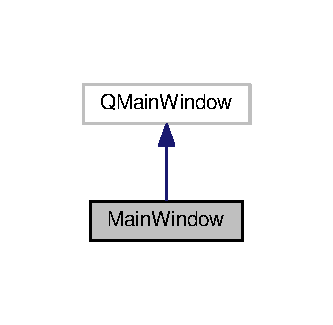
\includegraphics[width=160pt]{class_main_window__inherit__graph}
\end{center}
\end{figure}


Diagrama de colaboración para Main\+Window\+:\nopagebreak
\begin{figure}[H]
\begin{center}
\leavevmode
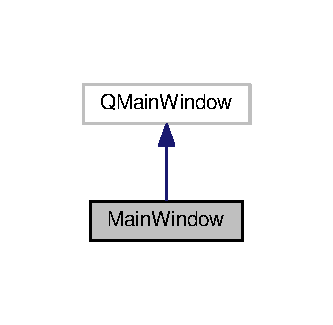
\includegraphics[width=160pt]{class_main_window__coll__graph}
\end{center}
\end{figure}
\subsection*{Métodos públicos}
\begin{DoxyCompactItemize}
\item 
\hyperlink{class_main_window_a8b244be8b7b7db1b08de2a2acb9409db}{Main\+Window} (Q\+Widget $\ast$parent=0)
\begin{DoxyCompactList}\small\item\em \hyperlink{class_main_window}{Main\+Window}. \end{DoxyCompactList}\end{DoxyCompactItemize}
\subsection*{Campos de datos}
\begin{DoxyCompactItemize}
\item 
Dyn\+Set\+Tree$<$ \hyperlink{class_event}{Event}, Avl\+\_\+\+Tree $>$ {\bfseries event\+Tree}\hypertarget{class_main_window_adb0e2b6f47127b9bf6abea1f234cfd3a}{}\label{class_main_window_adb0e2b6f47127b9bf6abea1f234cfd3a}

\end{DoxyCompactItemize}


\subsection{Descripción detallada}
Clase \hyperlink{class_main_window}{Main\+Window}. 

Definición en la línea 24 del archivo mainwindow.\+h.



\subsection{Documentación del constructor y destructor}
\index{Main\+Window@{Main\+Window}!Main\+Window@{Main\+Window}}
\index{Main\+Window@{Main\+Window}!Main\+Window@{Main\+Window}}
\subsubsection[{\texorpdfstring{Main\+Window(\+Q\+Widget $\ast$parent=0)}{MainWindow(QWidget *parent=0)}}]{\setlength{\rightskip}{0pt plus 5cm}Main\+Window\+::\+Main\+Window (
\begin{DoxyParamCaption}
\item[{Q\+Widget $\ast$}]{parent = {\ttfamily 0}}
\end{DoxyParamCaption}
)\hspace{0.3cm}{\ttfamily [explicit]}}\hypertarget{class_main_window_a8b244be8b7b7db1b08de2a2acb9409db}{}\label{class_main_window_a8b244be8b7b7db1b08de2a2acb9409db}


\hyperlink{class_main_window}{Main\+Window}. 


\begin{DoxyParams}{Parámetros}
{\em parent} & padre de componentes \\
\hline
\end{DoxyParams}


Definición en la línea 12 del archivo mainwindow.\+cpp.



La documentación para esta clase fue generada a partir de los siguientes ficheros\+:\begin{DoxyCompactItemize}
\item 
/home/eduuardoperez/pr3/championship-\/\+P\+R3\+\_\+\+U\+L\+A/project/\hyperlink{mainwindow_8h}{mainwindow.\+h}\item 
/home/eduuardoperez/pr3/championship-\/\+P\+R3\+\_\+\+U\+L\+A/project/\hyperlink{mainwindow_8cpp}{mainwindow.\+cpp}\end{DoxyCompactItemize}

\hypertarget{class_mod_event_window}{}\section{Referencia de la Clase Mod\+Event\+Window}
\label{class_mod_event_window}\index{Mod\+Event\+Window@{Mod\+Event\+Window}}


Clase \hyperlink{class_mod_event_window}{Mod\+Event\+Window}.  




{\ttfamily \#include $<$modeventwindow.\+h$>$}



Diagrama de herencias de Mod\+Event\+Window\nopagebreak
\begin{figure}[H]
\begin{center}
\leavevmode
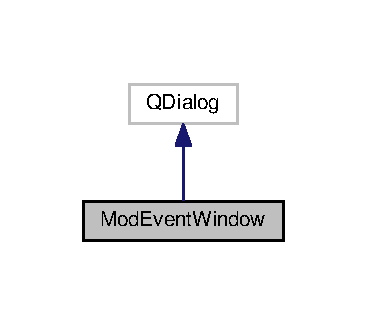
\includegraphics[width=176pt]{class_mod_event_window__inherit__graph}
\end{center}
\end{figure}


Diagrama de colaboración para Mod\+Event\+Window\+:\nopagebreak
\begin{figure}[H]
\begin{center}
\leavevmode
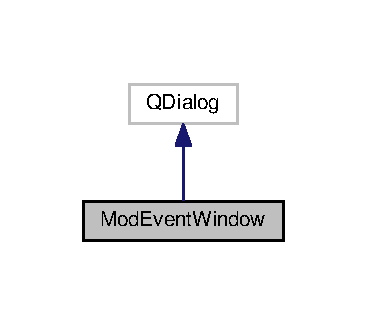
\includegraphics[width=176pt]{class_mod_event_window__coll__graph}
\end{center}
\end{figure}
\subsection*{Métodos públicos}
\begin{DoxyCompactItemize}
\item 
\hyperlink{class_mod_event_window_af82d1d1a727a13d06d33500f897bd2b2}{Mod\+Event\+Window} (Q\+Widget $\ast$parent=0)
\begin{DoxyCompactList}\small\item\em \hyperlink{class_mod_event_window}{Mod\+Event\+Window}. \end{DoxyCompactList}\end{DoxyCompactItemize}


\subsection{Descripción detallada}
Clase \hyperlink{class_mod_event_window}{Mod\+Event\+Window}. 

Definición en la línea 23 del archivo modeventwindow.\+h.



\subsection{Documentación del constructor y destructor}
\index{Mod\+Event\+Window@{Mod\+Event\+Window}!Mod\+Event\+Window@{Mod\+Event\+Window}}
\index{Mod\+Event\+Window@{Mod\+Event\+Window}!Mod\+Event\+Window@{Mod\+Event\+Window}}
\subsubsection[{\texorpdfstring{Mod\+Event\+Window(\+Q\+Widget $\ast$parent=0)}{ModEventWindow(QWidget *parent=0)}}]{\setlength{\rightskip}{0pt plus 5cm}Mod\+Event\+Window\+::\+Mod\+Event\+Window (
\begin{DoxyParamCaption}
\item[{Q\+Widget $\ast$}]{parent = {\ttfamily 0}}
\end{DoxyParamCaption}
)\hspace{0.3cm}{\ttfamily [explicit]}}\hypertarget{class_mod_event_window_af82d1d1a727a13d06d33500f897bd2b2}{}\label{class_mod_event_window_af82d1d1a727a13d06d33500f897bd2b2}


\hyperlink{class_mod_event_window}{Mod\+Event\+Window}. 


\begin{DoxyParams}{Parámetros}
{\em parent} & padre de componentes \\
\hline
\end{DoxyParams}


Definición en la línea 11 del archivo modeventwindow.\+cpp.



La documentación para esta clase fue generada a partir de los siguientes ficheros\+:\begin{DoxyCompactItemize}
\item 
/home/eduuardoperez/pr3/championship-\/\+P\+R3\+\_\+\+U\+L\+A/project/\hyperlink{modeventwindow_8h}{modeventwindow.\+h}\item 
/home/eduuardoperez/pr3/championship-\/\+P\+R3\+\_\+\+U\+L\+A/project/\hyperlink{modeventwindow_8cpp}{modeventwindow.\+cpp}\end{DoxyCompactItemize}

\hypertarget{class_organizing_window}{}\section{Referencia de la Clase Organizing\+Window}
\label{class_organizing_window}\index{Organizing\+Window@{Organizing\+Window}}


Clase \hyperlink{class_organizing_window}{Organizing\+Window}.  




{\ttfamily \#include $<$organizingwindow.\+h$>$}



Diagrama de herencias de Organizing\+Window\nopagebreak
\begin{figure}[H]
\begin{center}
\leavevmode
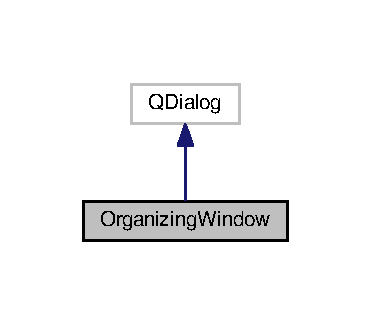
\includegraphics[width=178pt]{class_organizing_window__inherit__graph}
\end{center}
\end{figure}


Diagrama de colaboración para Organizing\+Window\+:\nopagebreak
\begin{figure}[H]
\begin{center}
\leavevmode
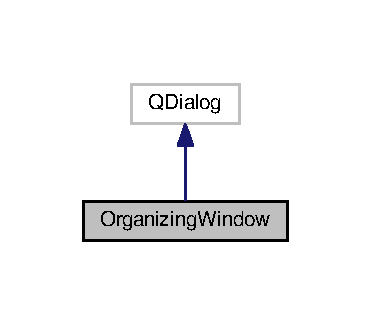
\includegraphics[width=178pt]{class_organizing_window__coll__graph}
\end{center}
\end{figure}
\subsection*{Métodos públicos}
\begin{DoxyCompactItemize}
\item 
\hyperlink{class_organizing_window_ac364fadd69b47d7ce67af56b8019c896}{Organizing\+Window} (Dyn\+Set\+Tree$<$ \hyperlink{class_event}{Event}, Avl\+\_\+\+Tree $>$ \&\hyperlink{class_organizing_window_a2658600a27160da36da9a20584300aac}{event\+Tree}, Q\+Widget $\ast$parent=0)
\begin{DoxyCompactList}\small\item\em \hyperlink{class_organizing_window}{Organizing\+Window}. \end{DoxyCompactList}\end{DoxyCompactItemize}
\subsection*{Campos de datos}
\begin{DoxyCompactItemize}
\item 
Dyn\+Set\+Tree$<$ \hyperlink{class_event}{Event}, Avl\+\_\+\+Tree $>$ $\ast$ \hyperlink{class_organizing_window_a2658600a27160da36da9a20584300aac}{event\+Tree}\hypertarget{class_organizing_window_a2658600a27160da36da9a20584300aac}{}\label{class_organizing_window_a2658600a27160da36da9a20584300aac}

\begin{DoxyCompactList}\small\item\em event\+Tree árbol para administrar los eventos \end{DoxyCompactList}\end{DoxyCompactItemize}


\subsection{Descripción detallada}
Clase \hyperlink{class_organizing_window}{Organizing\+Window}. 

Definición en la línea 26 del archivo organizingwindow.\+h.



\subsection{Documentación del constructor y destructor}
\index{Organizing\+Window@{Organizing\+Window}!Organizing\+Window@{Organizing\+Window}}
\index{Organizing\+Window@{Organizing\+Window}!Organizing\+Window@{Organizing\+Window}}
\subsubsection[{\texorpdfstring{Organizing\+Window(\+Dyn\+Set\+Tree$<$ Event, Avl\+\_\+\+Tree $>$ \&event\+Tree, Q\+Widget $\ast$parent=0)}{OrganizingWindow(DynSetTree< Event, Avl_Tree > &eventTree, QWidget *parent=0)}}]{\setlength{\rightskip}{0pt plus 5cm}Organizing\+Window\+::\+Organizing\+Window (
\begin{DoxyParamCaption}
\item[{Dyn\+Set\+Tree$<$ {\bf Event}, Avl\+\_\+\+Tree $>$ \&}]{event\+Tree, }
\item[{Q\+Widget $\ast$}]{parent = {\ttfamily 0}}
\end{DoxyParamCaption}
)\hspace{0.3cm}{\ttfamily [explicit]}}\hypertarget{class_organizing_window_ac364fadd69b47d7ce67af56b8019c896}{}\label{class_organizing_window_ac364fadd69b47d7ce67af56b8019c896}


\hyperlink{class_organizing_window}{Organizing\+Window}. 


\begin{DoxyParams}{Parámetros}
{\em event\+Tree} & árbol para administrar los eventos \\
\hline
{\em parent} & padre de componentes \\
\hline
\end{DoxyParams}


Definición en la línea 12 del archivo organizingwindow.\+cpp.



La documentación para esta clase fue generada a partir de los siguientes ficheros\+:\begin{DoxyCompactItemize}
\item 
/home/eduuardoperez/pr3/championship-\/\+P\+R3\+\_\+\+U\+L\+A/project/\hyperlink{organizingwindow_8h}{organizingwindow.\+h}\item 
/home/eduuardoperez/pr3/championship-\/\+P\+R3\+\_\+\+U\+L\+A/project/\hyperlink{organizingwindow_8cpp}{organizingwindow.\+cpp}\end{DoxyCompactItemize}

\hypertarget{class_participant}{}\section{Referencia de la Clase Participant}
\label{class_participant}\index{Participant@{Participant}}


Clase \hyperlink{class_participant}{Participant}.  




{\ttfamily \#include $<$participant.\+h$>$}

\subsection*{Métodos públicos}
\begin{DoxyCompactItemize}
\item 
\hyperlink{class_participant_a09e54ccec8ebca53dfb49c240b6d1ecd}{Participant} (const \hyperlink{class_participant}{Participant} \&)\hypertarget{class_participant_a09e54ccec8ebca53dfb49c240b6d1ecd}{}\label{class_participant_a09e54ccec8ebca53dfb49c240b6d1ecd}

\begin{DoxyCompactList}\small\item\em Constructor por copia de la clase \hyperlink{class_participant}{Participant}. \end{DoxyCompactList}\item 
unsigned int \hyperlink{class_participant_a7242a5ed6ceeba1b988297b4b1a29d2a}{get\+Id} () const 
\begin{DoxyCompactList}\small\item\em Observador get\+Id. \end{DoxyCompactList}\item 
string \hyperlink{class_participant_ae2fba0dcb273c86fbb3f295ca3c2a2b3}{get\+Name} () const 
\begin{DoxyCompactList}\small\item\em Observador get\+Name. \end{DoxyCompactList}\item 
string \hyperlink{class_participant_a9c05497ee615701e9f27c7114cf489be}{get\+Last\+Name} () const 
\begin{DoxyCompactList}\small\item\em Observador get\+Last\+Name. \end{DoxyCompactList}\item 
\hyperlink{class_date}{Date} \hyperlink{class_participant_ad969a57fb589033f35fbe82f57a8b765}{get\+Born\+Date} () const 
\begin{DoxyCompactList}\small\item\em Observador get\+Born\+Date. \end{DoxyCompactList}\item 
unsigned int \hyperlink{class_participant_afa2be326323515c15d8aaed642907680}{get\+Age} () const 
\begin{DoxyCompactList}\small\item\em Observador get\+Age. \end{DoxyCompactList}\item 
string \hyperlink{class_participant_a14ab6b07cc3e632fa353d15ecabcab8b}{get\+Category} () const 
\begin{DoxyCompactList}\small\item\em Observador get\+Category. \end{DoxyCompactList}\item 
\hyperlink{class_date}{Date} \hyperlink{class_participant_a0d720e44b2611994d03a7f8de682e414}{get\+Inscription\+Date} () const 
\begin{DoxyCompactList}\small\item\em Observador get\+Inscription\+Date. \end{DoxyCompactList}\item 
string \hyperlink{class_participant_a72fd0d83aa250c01a2f438deee6d0a37}{get\+Picture} () const 
\begin{DoxyCompactList}\small\item\em Observador get\+Picture. \end{DoxyCompactList}\item 
void \hyperlink{class_participant_a180a58ee8ad5b7c6ea8981bdd5697ed6}{set\+Id} (unsigned int)\hypertarget{class_participant_a180a58ee8ad5b7c6ea8981bdd5697ed6}{}\label{class_participant_a180a58ee8ad5b7c6ea8981bdd5697ed6}

\begin{DoxyCompactList}\small\item\em Modificador set\+Id. \end{DoxyCompactList}\item 
void \hyperlink{class_participant_a57c6abad16681cf90ad7e6afaaa197ca}{set\+Name} (string)\hypertarget{class_participant_a57c6abad16681cf90ad7e6afaaa197ca}{}\label{class_participant_a57c6abad16681cf90ad7e6afaaa197ca}

\begin{DoxyCompactList}\small\item\em Modificador set\+Name. \end{DoxyCompactList}\item 
void \hyperlink{class_participant_af885b7075cc7765a25a612a52301c382}{set\+Last\+Name} (string)\hypertarget{class_participant_af885b7075cc7765a25a612a52301c382}{}\label{class_participant_af885b7075cc7765a25a612a52301c382}

\begin{DoxyCompactList}\small\item\em Modificador set\+Last\+Name. \end{DoxyCompactList}\item 
void \hyperlink{class_participant_a92d064eb8d903317d0b4f0240a4fb08f}{set\+Born\+Date} (\hyperlink{class_date}{Date})\hypertarget{class_participant_a92d064eb8d903317d0b4f0240a4fb08f}{}\label{class_participant_a92d064eb8d903317d0b4f0240a4fb08f}

\begin{DoxyCompactList}\small\item\em Modificador set\+Born\+Date. \end{DoxyCompactList}\item 
void \hyperlink{class_participant_a4de112fc8f335175bbb9997c7440785e}{set\+Age} (unsigned int)\hypertarget{class_participant_a4de112fc8f335175bbb9997c7440785e}{}\label{class_participant_a4de112fc8f335175bbb9997c7440785e}

\begin{DoxyCompactList}\small\item\em Modificador set\+Age. \end{DoxyCompactList}\item 
void \hyperlink{class_participant_af91cf9adf356fa0f0c0cf8c9fe76a294}{set\+Category} (string)\hypertarget{class_participant_af91cf9adf356fa0f0c0cf8c9fe76a294}{}\label{class_participant_af91cf9adf356fa0f0c0cf8c9fe76a294}

\begin{DoxyCompactList}\small\item\em Modificador set\+Category. \end{DoxyCompactList}\item 
void \hyperlink{class_participant_ab8b20c06f6ef4f9a93c3a0eb4aa486f6}{set\+Inscription\+Date} (\hyperlink{class_date}{Date})\hypertarget{class_participant_ab8b20c06f6ef4f9a93c3a0eb4aa486f6}{}\label{class_participant_ab8b20c06f6ef4f9a93c3a0eb4aa486f6}

\begin{DoxyCompactList}\small\item\em Modificador set\+Inscription\+Date. \end{DoxyCompactList}\item 
void \hyperlink{class_participant_a8ed3db539a1ab6c04b110968347f45fb}{set\+Picture} (string)\hypertarget{class_participant_a8ed3db539a1ab6c04b110968347f45fb}{}\label{class_participant_a8ed3db539a1ab6c04b110968347f45fb}

\begin{DoxyCompactList}\small\item\em Modificador set\+Picture. \end{DoxyCompactList}\item 
void \hyperlink{class_participant_aacee4e07ebfe68b4521217b2c3b6dbf5}{assign} (unsigned int, string, string, \hyperlink{class_date}{Date}, unsigned int, string, \hyperlink{class_date}{Date}, string)\hypertarget{class_participant_aacee4e07ebfe68b4521217b2c3b6dbf5}{}\label{class_participant_aacee4e07ebfe68b4521217b2c3b6dbf5}

\begin{DoxyCompactList}\small\item\em Método assign. \end{DoxyCompactList}\item 
\hyperlink{class_participant}{Participant} \hyperlink{class_participant_af7f2abaadf20275a00ef287ec81ca546}{operator=} (const \hyperlink{class_participant}{Participant} \&)
\begin{DoxyCompactList}\small\item\em operator = \end{DoxyCompactList}\item 
int \hyperlink{class_participant_a847dfbbd072f49e67a5b30d549c2e616}{operator==} (const \hyperlink{class_participant}{Participant} \&)
\begin{DoxyCompactList}\small\item\em operator == \end{DoxyCompactList}\end{DoxyCompactItemize}


\subsection{Descripción detallada}
Clase \hyperlink{class_participant}{Participant}. 

Definición en la línea 18 del archivo participant.\+h.



\subsection{Documentación de las funciones miembro}
\index{Participant@{Participant}!get\+Age@{get\+Age}}
\index{get\+Age@{get\+Age}!Participant@{Participant}}
\subsubsection[{\texorpdfstring{get\+Age() const }{getAge() const }}]{\setlength{\rightskip}{0pt plus 5cm}unsigned int Participant\+::get\+Age (
\begin{DoxyParamCaption}
{}
\end{DoxyParamCaption}
) const\hspace{0.3cm}{\ttfamily [inline]}}\hypertarget{class_participant_afa2be326323515c15d8aaed642907680}{}\label{class_participant_afa2be326323515c15d8aaed642907680}


Observador get\+Age. 

\begin{DoxyReturn}{Devuelve}
this-\/$>$age 
\end{DoxyReturn}


Definición en la línea 80 del archivo participant.\+h.

\index{Participant@{Participant}!get\+Born\+Date@{get\+Born\+Date}}
\index{get\+Born\+Date@{get\+Born\+Date}!Participant@{Participant}}
\subsubsection[{\texorpdfstring{get\+Born\+Date() const }{getBornDate() const }}]{\setlength{\rightskip}{0pt plus 5cm}{\bf Date} Participant\+::get\+Born\+Date (
\begin{DoxyParamCaption}
{}
\end{DoxyParamCaption}
) const\hspace{0.3cm}{\ttfamily [inline]}}\hypertarget{class_participant_ad969a57fb589033f35fbe82f57a8b765}{}\label{class_participant_ad969a57fb589033f35fbe82f57a8b765}


Observador get\+Born\+Date. 

\begin{DoxyReturn}{Devuelve}
this-\/$>$born\+Date 
\end{DoxyReturn}


Definición en la línea 71 del archivo participant.\+h.

\index{Participant@{Participant}!get\+Category@{get\+Category}}
\index{get\+Category@{get\+Category}!Participant@{Participant}}
\subsubsection[{\texorpdfstring{get\+Category() const }{getCategory() const }}]{\setlength{\rightskip}{0pt plus 5cm}string Participant\+::get\+Category (
\begin{DoxyParamCaption}
{}
\end{DoxyParamCaption}
) const\hspace{0.3cm}{\ttfamily [inline]}}\hypertarget{class_participant_a14ab6b07cc3e632fa353d15ecabcab8b}{}\label{class_participant_a14ab6b07cc3e632fa353d15ecabcab8b}


Observador get\+Category. 

\begin{DoxyReturn}{Devuelve}
this-\/$>$category 
\end{DoxyReturn}


Definición en la línea 89 del archivo participant.\+h.

\index{Participant@{Participant}!get\+Id@{get\+Id}}
\index{get\+Id@{get\+Id}!Participant@{Participant}}
\subsubsection[{\texorpdfstring{get\+Id() const }{getId() const }}]{\setlength{\rightskip}{0pt plus 5cm}unsigned int Participant\+::get\+Id (
\begin{DoxyParamCaption}
{}
\end{DoxyParamCaption}
) const\hspace{0.3cm}{\ttfamily [inline]}}\hypertarget{class_participant_a7242a5ed6ceeba1b988297b4b1a29d2a}{}\label{class_participant_a7242a5ed6ceeba1b988297b4b1a29d2a}


Observador get\+Id. 

\begin{DoxyReturn}{Devuelve}
this-\/$>$id 
\end{DoxyReturn}


Definición en la línea 44 del archivo participant.\+h.

\index{Participant@{Participant}!get\+Inscription\+Date@{get\+Inscription\+Date}}
\index{get\+Inscription\+Date@{get\+Inscription\+Date}!Participant@{Participant}}
\subsubsection[{\texorpdfstring{get\+Inscription\+Date() const }{getInscriptionDate() const }}]{\setlength{\rightskip}{0pt plus 5cm}{\bf Date} Participant\+::get\+Inscription\+Date (
\begin{DoxyParamCaption}
{}
\end{DoxyParamCaption}
) const\hspace{0.3cm}{\ttfamily [inline]}}\hypertarget{class_participant_a0d720e44b2611994d03a7f8de682e414}{}\label{class_participant_a0d720e44b2611994d03a7f8de682e414}


Observador get\+Inscription\+Date. 

\begin{DoxyReturn}{Devuelve}
this-\/$>$inscription\+Date 
\end{DoxyReturn}


Definición en la línea 98 del archivo participant.\+h.

\index{Participant@{Participant}!get\+Last\+Name@{get\+Last\+Name}}
\index{get\+Last\+Name@{get\+Last\+Name}!Participant@{Participant}}
\subsubsection[{\texorpdfstring{get\+Last\+Name() const }{getLastName() const }}]{\setlength{\rightskip}{0pt plus 5cm}string Participant\+::get\+Last\+Name (
\begin{DoxyParamCaption}
{}
\end{DoxyParamCaption}
) const\hspace{0.3cm}{\ttfamily [inline]}}\hypertarget{class_participant_a9c05497ee615701e9f27c7114cf489be}{}\label{class_participant_a9c05497ee615701e9f27c7114cf489be}


Observador get\+Last\+Name. 

\begin{DoxyReturn}{Devuelve}
this-\/$>$last\+Name 
\end{DoxyReturn}


Definición en la línea 62 del archivo participant.\+h.

\index{Participant@{Participant}!get\+Name@{get\+Name}}
\index{get\+Name@{get\+Name}!Participant@{Participant}}
\subsubsection[{\texorpdfstring{get\+Name() const }{getName() const }}]{\setlength{\rightskip}{0pt plus 5cm}string Participant\+::get\+Name (
\begin{DoxyParamCaption}
{}
\end{DoxyParamCaption}
) const\hspace{0.3cm}{\ttfamily [inline]}}\hypertarget{class_participant_ae2fba0dcb273c86fbb3f295ca3c2a2b3}{}\label{class_participant_ae2fba0dcb273c86fbb3f295ca3c2a2b3}


Observador get\+Name. 

\begin{DoxyReturn}{Devuelve}
this-\/$>$name 
\end{DoxyReturn}


Definición en la línea 53 del archivo participant.\+h.

\index{Participant@{Participant}!get\+Picture@{get\+Picture}}
\index{get\+Picture@{get\+Picture}!Participant@{Participant}}
\subsubsection[{\texorpdfstring{get\+Picture() const }{getPicture() const }}]{\setlength{\rightskip}{0pt plus 5cm}string Participant\+::get\+Picture (
\begin{DoxyParamCaption}
{}
\end{DoxyParamCaption}
) const\hspace{0.3cm}{\ttfamily [inline]}}\hypertarget{class_participant_a72fd0d83aa250c01a2f438deee6d0a37}{}\label{class_participant_a72fd0d83aa250c01a2f438deee6d0a37}


Observador get\+Picture. 

\begin{DoxyReturn}{Devuelve}
dirección lógica de this-\/$>$picture 
\end{DoxyReturn}


Definición en la línea 107 del archivo participant.\+h.

\index{Participant@{Participant}!operator=@{operator=}}
\index{operator=@{operator=}!Participant@{Participant}}
\subsubsection[{\texorpdfstring{operator=(const Participant \&)}{operator=(const Participant &)}}]{\setlength{\rightskip}{0pt plus 5cm}{\bf Participant} Participant\+::operator= (
\begin{DoxyParamCaption}
\item[{const {\bf Participant} \&}]{participant}
\end{DoxyParamCaption}
)}\hypertarget{class_participant_af7f2abaadf20275a00ef287ec81ca546}{}\label{class_participant_af7f2abaadf20275a00ef287ec81ca546}


operator = 

\begin{DoxyReturn}{Devuelve}
\hyperlink{class_participant}{Participant} participant 
\end{DoxyReturn}


Definición en la línea 97 del archivo participant.\+cpp.

\index{Participant@{Participant}!operator==@{operator==}}
\index{operator==@{operator==}!Participant@{Participant}}
\subsubsection[{\texorpdfstring{operator==(const Participant \&)}{operator==(const Participant &)}}]{\setlength{\rightskip}{0pt plus 5cm}int Participant\+::operator== (
\begin{DoxyParamCaption}
\item[{const {\bf Participant} \&}]{participant}
\end{DoxyParamCaption}
)}\hypertarget{class_participant_a847dfbbd072f49e67a5b30d549c2e616}{}\label{class_participant_a847dfbbd072f49e67a5b30d549c2e616}


operator == 

\begin{DoxyReturn}{Devuelve}
1 si this es igual a participant, 0 si no lo es. 
\end{DoxyReturn}


Definición en la línea 110 del archivo participant.\+cpp.



La documentación para esta clase fue generada a partir de los siguientes ficheros\+:\begin{DoxyCompactItemize}
\item 
/home/eduuardoperez/pr3/championship-\/\+P\+R3\+\_\+\+U\+L\+A/project/\hyperlink{participant_8h}{participant.\+h}\item 
/home/eduuardoperez/pr3/championship-\/\+P\+R3\+\_\+\+U\+L\+A/project/\hyperlink{participant_8cpp}{participant.\+cpp}\end{DoxyCompactItemize}

\hypertarget{class_reg_event_window}{}\section{Referencia de la Clase Reg\+Event\+Window}
\label{class_reg_event_window}\index{Reg\+Event\+Window@{Reg\+Event\+Window}}


Clase \hyperlink{class_reg_event_window}{Reg\+Event\+Window}.  




{\ttfamily \#include $<$regeventwindow.\+h$>$}



Diagrama de herencias de Reg\+Event\+Window\nopagebreak
\begin{figure}[H]
\begin{center}
\leavevmode
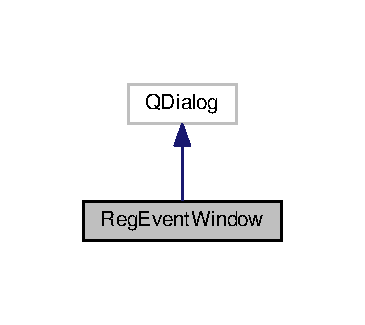
\includegraphics[width=175pt]{class_reg_event_window__inherit__graph}
\end{center}
\end{figure}


Diagrama de colaboración para Reg\+Event\+Window\+:\nopagebreak
\begin{figure}[H]
\begin{center}
\leavevmode
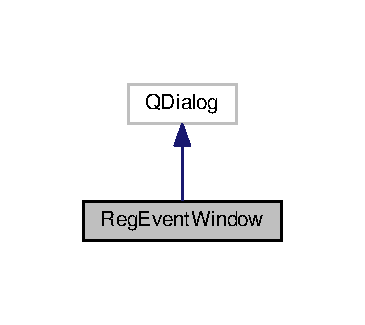
\includegraphics[width=175pt]{class_reg_event_window__coll__graph}
\end{center}
\end{figure}
\subsection*{Métodos públicos}
\begin{DoxyCompactItemize}
\item 
\hyperlink{class_reg_event_window_a2985bc88d5498d00e66bd124d007dc2c}{Reg\+Event\+Window} (Q\+Widget $\ast$parent=0)
\begin{DoxyCompactList}\small\item\em \hyperlink{class_reg_event_window}{Reg\+Event\+Window}. \end{DoxyCompactList}\end{DoxyCompactItemize}


\subsection{Descripción detallada}
Clase \hyperlink{class_reg_event_window}{Reg\+Event\+Window}. 

Definición en la línea 30 del archivo regeventwindow.\+h.



\subsection{Documentación del constructor y destructor}
\index{Reg\+Event\+Window@{Reg\+Event\+Window}!Reg\+Event\+Window@{Reg\+Event\+Window}}
\index{Reg\+Event\+Window@{Reg\+Event\+Window}!Reg\+Event\+Window@{Reg\+Event\+Window}}
\subsubsection[{\texorpdfstring{Reg\+Event\+Window(\+Q\+Widget $\ast$parent=0)}{RegEventWindow(QWidget *parent=0)}}]{\setlength{\rightskip}{0pt plus 5cm}Reg\+Event\+Window\+::\+Reg\+Event\+Window (
\begin{DoxyParamCaption}
\item[{Q\+Widget $\ast$}]{parent = {\ttfamily 0}}
\end{DoxyParamCaption}
)\hspace{0.3cm}{\ttfamily [explicit]}}\hypertarget{class_reg_event_window_a2985bc88d5498d00e66bd124d007dc2c}{}\label{class_reg_event_window_a2985bc88d5498d00e66bd124d007dc2c}


\hyperlink{class_reg_event_window}{Reg\+Event\+Window}. 


\begin{DoxyParams}{Parámetros}
{\em parent} & padre de componentes \\
\hline
\end{DoxyParams}


Definición en la línea 12 del archivo regeventwindow.\+cpp.



La documentación para esta clase fue generada a partir de los siguientes ficheros\+:\begin{DoxyCompactItemize}
\item 
/home/eduuardoperez/pr3/championship-\/\+P\+R3\+\_\+\+U\+L\+A/project/\hyperlink{regeventwindow_8h}{regeventwindow.\+h}\item 
/home/eduuardoperez/pr3/championship-\/\+P\+R3\+\_\+\+U\+L\+A/project/\hyperlink{regeventwindow_8cpp}{regeventwindow.\+cpp}\end{DoxyCompactItemize}

\hypertarget{class_sporty_window}{}\section{Referencia de la Clase Sporty\+Window}
\label{class_sporty_window}\index{Sporty\+Window@{Sporty\+Window}}


Clase \hyperlink{class_sporty_window}{Sporty\+Window}.  




{\ttfamily \#include $<$sportywindow.\+h$>$}



Diagrama de herencias de Sporty\+Window\nopagebreak
\begin{figure}[H]
\begin{center}
\leavevmode
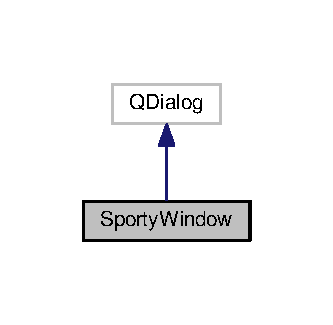
\includegraphics[width=160pt]{class_sporty_window__inherit__graph}
\end{center}
\end{figure}


Diagrama de colaboración para Sporty\+Window\+:\nopagebreak
\begin{figure}[H]
\begin{center}
\leavevmode
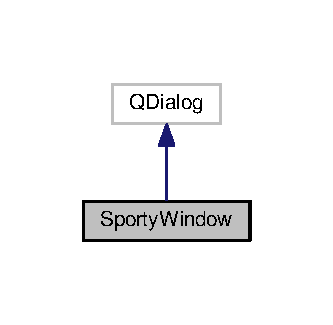
\includegraphics[width=160pt]{class_sporty_window__coll__graph}
\end{center}
\end{figure}
\subsection*{Métodos públicos}
\begin{DoxyCompactItemize}
\item 
\hyperlink{class_sporty_window_aefcc1a9246b5509f53ccd6f2bc5fd71d}{Sporty\+Window} (Dyn\+Set\+Tree$<$ \hyperlink{class_event}{Event}, Avl\+\_\+\+Tree $>$ \&\hyperlink{class_sporty_window_ae5042630126b218d12b7f7b9b92c4307}{event\+Tree}, Dyn\+Set\+Tree$<$ string, Avl\+\_\+\+Tree $>$ \&\hyperlink{class_sporty_window_a1d1ad05d15c5b535772652e0f72afe04}{nm\+Ev\+Tree}, Dyn\+Set\+Tree$<$ \hyperlink{class_participant}{Participant}, Avl\+\_\+\+Tree $>$ \&\hyperlink{class_sporty_window_affb306650ea3c48ad8ffc219dcc8c0f7}{part\+Tree}, Dyn\+Set\+Tree$<$ Pair, Avl\+\_\+\+Tree $>$ \&\hyperlink{class_sporty_window_a042928055a5216651908f3797c1fc6e6}{ev\+Part\+Tree}, Q\+Widget $\ast$parent=0)
\begin{DoxyCompactList}\small\item\em \hyperlink{class_sporty_window}{Sporty\+Window}. \end{DoxyCompactList}\end{DoxyCompactItemize}
\subsection*{Campos de datos}
\begin{DoxyCompactItemize}
\item 
Dyn\+Set\+Tree$<$ \hyperlink{class_event}{Event}, Avl\+\_\+\+Tree $>$ $\ast$ \hyperlink{class_sporty_window_ae5042630126b218d12b7f7b9b92c4307}{event\+Tree}\hypertarget{class_sporty_window_ae5042630126b218d12b7f7b9b92c4307}{}\label{class_sporty_window_ae5042630126b218d12b7f7b9b92c4307}

\begin{DoxyCompactList}\small\item\em event\+Tree árbol para administrar los eventos \end{DoxyCompactList}\item 
Dyn\+Set\+Tree$<$ string, Avl\+\_\+\+Tree $>$ $\ast$ \hyperlink{class_sporty_window_a1d1ad05d15c5b535772652e0f72afe04}{nm\+Ev\+Tree}\hypertarget{class_sporty_window_a1d1ad05d15c5b535772652e0f72afe04}{}\label{class_sporty_window_a1d1ad05d15c5b535772652e0f72afe04}

\begin{DoxyCompactList}\small\item\em nm\+Ev\+Tree árbol para administrar los nombres de los eventos \end{DoxyCompactList}\item 
Dyn\+Set\+Tree$<$ \hyperlink{class_participant}{Participant}, Avl\+\_\+\+Tree $>$ $\ast$ \hyperlink{class_sporty_window_affb306650ea3c48ad8ffc219dcc8c0f7}{part\+Tree}\hypertarget{class_sporty_window_affb306650ea3c48ad8ffc219dcc8c0f7}{}\label{class_sporty_window_affb306650ea3c48ad8ffc219dcc8c0f7}

\begin{DoxyCompactList}\small\item\em part\+Tree árbol para administrar los participantes \end{DoxyCompactList}\item 
Dyn\+Set\+Tree$<$ Pair, Avl\+\_\+\+Tree $>$ $\ast$ \hyperlink{class_sporty_window_a042928055a5216651908f3797c1fc6e6}{ev\+Part\+Tree}\hypertarget{class_sporty_window_a042928055a5216651908f3797c1fc6e6}{}\label{class_sporty_window_a042928055a5216651908f3797c1fc6e6}

\begin{DoxyCompactList}\small\item\em ev\+Part\+Tree árbol auxiliar para administrar los participantes \end{DoxyCompactList}\end{DoxyCompactItemize}


\subsection{Descripción detallada}
Clase \hyperlink{class_sporty_window}{Sporty\+Window}. 

Definición en la línea 29 del archivo sportywindow.\+h.



\subsection{Documentación del constructor y destructor}
\index{Sporty\+Window@{Sporty\+Window}!Sporty\+Window@{Sporty\+Window}}
\index{Sporty\+Window@{Sporty\+Window}!Sporty\+Window@{Sporty\+Window}}
\subsubsection[{\texorpdfstring{Sporty\+Window(\+Dyn\+Set\+Tree$<$ Event, Avl\+\_\+\+Tree $>$ \&event\+Tree, Dyn\+Set\+Tree$<$ string, Avl\+\_\+\+Tree $>$ \&nm\+Ev\+Tree, Dyn\+Set\+Tree$<$ Participant, Avl\+\_\+\+Tree $>$ \&part\+Tree, Dyn\+Set\+Tree$<$ Pair, Avl\+\_\+\+Tree $>$ \&ev\+Part\+Tree, Q\+Widget $\ast$parent=0)}{SportyWindow(DynSetTree< Event, Avl_Tree > &eventTree, DynSetTree< string, Avl_Tree > &nmEvTree, DynSetTree< Participant, Avl_Tree > &partTree, DynSetTree< Pair, Avl_Tree > &evPartTree, QWidget *parent=0)}}]{\setlength{\rightskip}{0pt plus 5cm}Sporty\+Window\+::\+Sporty\+Window (
\begin{DoxyParamCaption}
\item[{Dyn\+Set\+Tree$<$ {\bf Event}, Avl\+\_\+\+Tree $>$ \&}]{event\+Tree, }
\item[{Dyn\+Set\+Tree$<$ string, Avl\+\_\+\+Tree $>$ \&}]{nm\+Ev\+Tree, }
\item[{Dyn\+Set\+Tree$<$ {\bf Participant}, Avl\+\_\+\+Tree $>$ \&}]{part\+Tree, }
\item[{Dyn\+Set\+Tree$<$ Pair, Avl\+\_\+\+Tree $>$ \&}]{ev\+Part\+Tree, }
\item[{Q\+Widget $\ast$}]{parent = {\ttfamily 0}}
\end{DoxyParamCaption}
)\hspace{0.3cm}{\ttfamily [explicit]}}\hypertarget{class_sporty_window_aefcc1a9246b5509f53ccd6f2bc5fd71d}{}\label{class_sporty_window_aefcc1a9246b5509f53ccd6f2bc5fd71d}


\hyperlink{class_sporty_window}{Sporty\+Window}. 


\begin{DoxyParams}{Parámetros}
{\em event\+Tree} & árbol para administrar los eventos \\
\hline
{\em nm\+Ev\+Tree} & árbol para administrar los nombres de los eventos \\
\hline
{\em part\+Tree} & árbol para administrar los participantes \\
\hline
{\em ev\+Part\+Tree} & árbol auxiliar para administrar los participantes \\
\hline
{\em parent} & padre de componentes \\
\hline
\end{DoxyParams}


Definición en la línea 11 del archivo sportywindow.\+cpp.



La documentación para esta clase fue generada a partir de los siguientes ficheros\+:\begin{DoxyCompactItemize}
\item 
/home/eduuardoperez/pr3/championship-\/\+P\+R3\+\_\+\+U\+L\+A/project/\hyperlink{sportywindow_8h}{sportywindow.\+h}\item 
/home/eduuardoperez/pr3/championship-\/\+P\+R3\+\_\+\+U\+L\+A/project/\hyperlink{sportywindow_8cpp}{sportywindow.\+cpp}\end{DoxyCompactItemize}

\hypertarget{class_view_event}{}\section{Referencia de la Clase View\+Event}
\label{class_view_event}\index{View\+Event@{View\+Event}}


Clase \hyperlink{class_view_event}{View\+Event}.  




{\ttfamily \#include $<$vieweventwindow.\+h$>$}



Diagrama de herencias de View\+Event\nopagebreak
\begin{figure}[H]
\begin{center}
\leavevmode
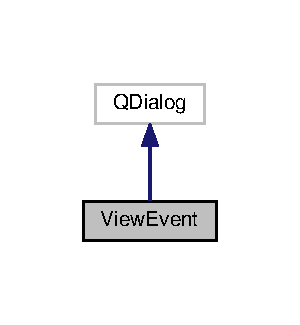
\includegraphics[width=144pt]{class_view_event__inherit__graph}
\end{center}
\end{figure}


Diagrama de colaboración para View\+Event\+:\nopagebreak
\begin{figure}[H]
\begin{center}
\leavevmode
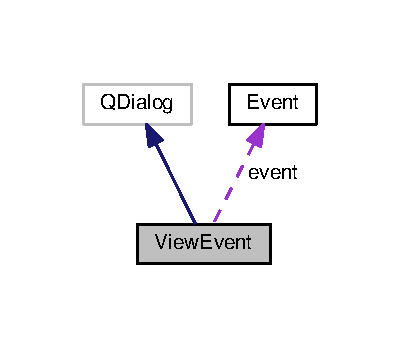
\includegraphics[width=192pt]{class_view_event__coll__graph}
\end{center}
\end{figure}
\subsection*{Métodos públicos}
\begin{DoxyCompactItemize}
\item 
\hyperlink{class_view_event_aa658be5ff516e8b7ba6f611ef350ce86}{View\+Event} (Dyn\+Set\+Tree$<$ \hyperlink{class_event}{Event}, Avl\+\_\+\+Tree $>$ $\ast$\hyperlink{class_view_event_a4a5575a712fa3139027258e5f2bb1201}{event\+Tree}, Dyn\+Set\+Tree$<$ string, Avl\+\_\+\+Tree $>$ $\ast$\hyperlink{class_view_event_a37f2e050e0d8b837d40bdaa6f81aab20}{nm\+Ev\+Tree}, const \hyperlink{class_event}{Event} \&\hyperlink{class_view_event_a3a9469ca9e317bfc5bce5d9341d0b2a1}{event}, Q\+Widget $\ast$parent=0)
\begin{DoxyCompactList}\small\item\em \hyperlink{class_view_event}{View\+Event}. \end{DoxyCompactList}\end{DoxyCompactItemize}
\subsection*{Campos de datos}
\begin{DoxyCompactItemize}
\item 
Dyn\+Set\+Tree$<$ \hyperlink{class_event}{Event}, Avl\+\_\+\+Tree $>$ $\ast$ \hyperlink{class_view_event_a4a5575a712fa3139027258e5f2bb1201}{event\+Tree}\hypertarget{class_view_event_a4a5575a712fa3139027258e5f2bb1201}{}\label{class_view_event_a4a5575a712fa3139027258e5f2bb1201}

\begin{DoxyCompactList}\small\item\em event\+Tree árbol para administrar los eventos \end{DoxyCompactList}\item 
Dyn\+Set\+Tree$<$ string, Avl\+\_\+\+Tree $>$ $\ast$ \hyperlink{class_view_event_a37f2e050e0d8b837d40bdaa6f81aab20}{nm\+Ev\+Tree}\hypertarget{class_view_event_a37f2e050e0d8b837d40bdaa6f81aab20}{}\label{class_view_event_a37f2e050e0d8b837d40bdaa6f81aab20}

\begin{DoxyCompactList}\small\item\em event\+Tree árbol para administrar los nombres de los eventos \end{DoxyCompactList}\item 
\hyperlink{class_event}{Event} \hyperlink{class_view_event_a3a9469ca9e317bfc5bce5d9341d0b2a1}{event}\hypertarget{class_view_event_a3a9469ca9e317bfc5bce5d9341d0b2a1}{}\label{class_view_event_a3a9469ca9e317bfc5bce5d9341d0b2a1}

\begin{DoxyCompactList}\small\item\em event event del cual se cargarán los datos en la ventana \end{DoxyCompactList}\end{DoxyCompactItemize}


\subsection{Descripción detallada}
Clase \hyperlink{class_view_event}{View\+Event}. 

Definición en la línea 14 del archivo vieweventwindow.\+h.



\subsection{Documentación del constructor y destructor}
\index{View\+Event@{View\+Event}!View\+Event@{View\+Event}}
\index{View\+Event@{View\+Event}!View\+Event@{View\+Event}}
\subsubsection[{\texorpdfstring{View\+Event(\+Dyn\+Set\+Tree$<$ Event, Avl\+\_\+\+Tree $>$ $\ast$event\+Tree, Dyn\+Set\+Tree$<$ string, Avl\+\_\+\+Tree $>$ $\ast$nm\+Ev\+Tree, const Event \&event, Q\+Widget $\ast$parent=0)}{ViewEvent(DynSetTree< Event, Avl_Tree > *eventTree, DynSetTree< string, Avl_Tree > *nmEvTree, const Event &event, QWidget *parent=0)}}]{\setlength{\rightskip}{0pt plus 5cm}View\+Event\+::\+View\+Event (
\begin{DoxyParamCaption}
\item[{Dyn\+Set\+Tree$<$ {\bf Event}, Avl\+\_\+\+Tree $>$ $\ast$}]{event\+Tree, }
\item[{Dyn\+Set\+Tree$<$ string, Avl\+\_\+\+Tree $>$ $\ast$}]{nm\+Ev\+Tree, }
\item[{const {\bf Event} \&}]{event, }
\item[{Q\+Widget $\ast$}]{parent = {\ttfamily 0}}
\end{DoxyParamCaption}
)\hspace{0.3cm}{\ttfamily [explicit]}}\hypertarget{class_view_event_aa658be5ff516e8b7ba6f611ef350ce86}{}\label{class_view_event_aa658be5ff516e8b7ba6f611ef350ce86}


\hyperlink{class_view_event}{View\+Event}. 


\begin{DoxyParams}{Parámetros}
{\em event\+Tree} & árbol para administrar los eventos \\
\hline
{\em nm\+Ev\+Tree} & árbol para administrar los nombres de los eventos \\
\hline
{\em event} & event del cual se cargarán los datos en la ventana \\
\hline
{\em parent} & padre de componentes \\
\hline
\end{DoxyParams}


Definición en la línea 4 del archivo vieweventwindow.\+cpp.



La documentación para esta clase fue generada a partir de los siguientes ficheros\+:\begin{DoxyCompactItemize}
\item 
/home/eduuardoperez/pr3/championship-\/\+P\+R3\+\_\+\+U\+L\+A/project/vieweventwindow.\+h\item 
/home/eduuardoperez/pr3/championship-\/\+P\+R3\+\_\+\+U\+L\+A/project/vieweventwindow.\+cpp\end{DoxyCompactItemize}

\chapter{Documentación de archivos}
\hypertarget{date_8cpp}{}\section{Referencia del Archivo /home/eduuardoperez/pr3/championship-\/\+P\+R3\+\_\+\+U\+L\+A/project/date.cpp}
\label{date_8cpp}\index{/home/eduuardoperez/pr3/championship-\/\+P\+R3\+\_\+\+U\+L\+A/project/date.\+cpp@{/home/eduuardoperez/pr3/championship-\/\+P\+R3\+\_\+\+U\+L\+A/project/date.\+cpp}}


Implementación de la clase \hyperlink{class_date}{Date}.  


{\ttfamily \#include \char`\"{}date.\+h\char`\"{}}\\*
Dependencia gráfica adjunta para date.\+cpp\+:\nopagebreak
\begin{figure}[H]
\begin{center}
\leavevmode
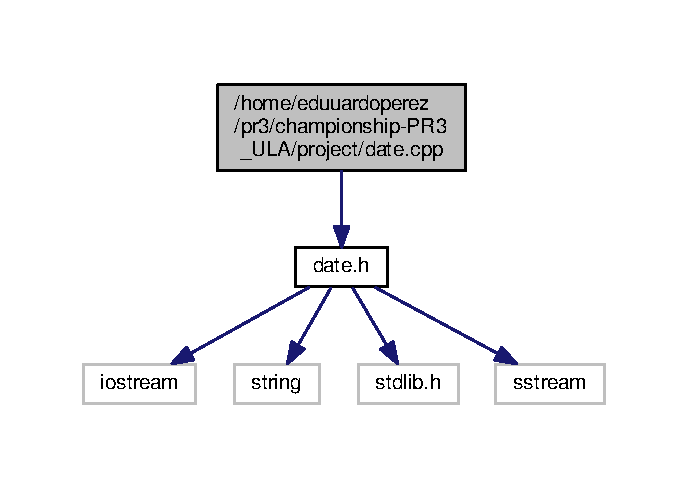
\includegraphics[width=330pt]{date_8cpp__incl}
\end{center}
\end{figure}
\subsection*{Funciones}
\begin{DoxyCompactItemize}
\item 
bool \hyperlink{date_8cpp_aa2e695ccf211714fafbc8c73cb7e5419}{operator$<$} (const \hyperlink{class_date}{Date} \&date1, const \hyperlink{class_date}{Date} \&date2)
\begin{DoxyCompactList}\small\item\em operator $<$ \end{DoxyCompactList}\item 
bool \hyperlink{date_8cpp_ad442d522a65d30aca55827a74ffd621d}{operator$>$} (const \hyperlink{class_date}{Date} \&date1, const \hyperlink{class_date}{Date} \&date2)
\begin{DoxyCompactList}\small\item\em operator $>$ \end{DoxyCompactList}\item 
bool \hyperlink{date_8cpp_a87454da328d25895944a03fba1e0aed1}{operator$<$=} (const \hyperlink{class_date}{Date} \&date1, const \hyperlink{class_date}{Date} \&date2)
\begin{DoxyCompactList}\small\item\em operator $<$= \end{DoxyCompactList}\item 
bool \hyperlink{date_8cpp_a5c20018c86b496cba7e7ed0dd5aee323}{operator$>$=} (const \hyperlink{class_date}{Date} \&date1, const \hyperlink{class_date}{Date} \&date2)
\begin{DoxyCompactList}\small\item\em operator $>$= \end{DoxyCompactList}\item 
ostream \& \hyperlink{date_8cpp_a525b2aeba34711c545cf51535c5a1fda}{operator$<$$<$} (ostream \&date, const \hyperlink{class_date}{Date} \&p)
\begin{DoxyCompactList}\small\item\em operator $<$$<$ \end{DoxyCompactList}\item 
istream \& \hyperlink{date_8cpp_a9f4b928e136b790da2fb7396829b8d51}{operator$>$$>$} (istream \&date, \hyperlink{class_date}{Date} \&aux)
\begin{DoxyCompactList}\small\item\em operator $>$$>$ \end{DoxyCompactList}\item 
string \hyperlink{date_8cpp_aa36788e1fe302221cb9446e85b88155f}{Uint2\+String} (unsigned int num)
\begin{DoxyCompactList}\small\item\em Método Uint2\+String. \end{DoxyCompactList}\end{DoxyCompactItemize}


\subsection{Descripción detallada}
Implementación de la clase \hyperlink{class_date}{Date}. 

\begin{DoxyAuthor}{Autor}
Eduardo Perez (\href{mailto:edujpp1@gmail.com}{\tt edujpp1@gmail.\+com}) 
\end{DoxyAuthor}
\begin{DoxyVersion}{Versión}
1.\+0 
\end{DoxyVersion}
\begin{DoxyDate}{Fecha}
Noviembre, 2016 
\end{DoxyDate}


\subsection{Documentación de las funciones}
\index{date.\+cpp@{date.\+cpp}!operator$<$@{operator$<$}}
\index{operator$<$@{operator$<$}!date.\+cpp@{date.\+cpp}}
\subsubsection[{\texorpdfstring{operator$<$(const Date \&date1, const Date \&date2)}{operator<(const Date &date1, const Date &date2)}}]{\setlength{\rightskip}{0pt plus 5cm}bool operator$<$ (
\begin{DoxyParamCaption}
\item[{const {\bf Date} \&}]{, }
\item[{const {\bf Date} \&}]{}
\end{DoxyParamCaption}
)}\hypertarget{date_8cpp_aa2e695ccf211714fafbc8c73cb7e5419}{}\label{date_8cpp_aa2e695ccf211714fafbc8c73cb7e5419}


operator $<$ 

\begin{DoxyReturn}{Devuelve}
true si this es menor a date, false de lo contrario. 
\end{DoxyReturn}


Definición en la línea 107 del archivo date.\+cpp.

\index{date.\+cpp@{date.\+cpp}!operator$<$$<$@{operator$<$$<$}}
\index{operator$<$$<$@{operator$<$$<$}!date.\+cpp@{date.\+cpp}}
\subsubsection[{\texorpdfstring{operator$<$$<$(ostream \&date, const Date \&p)}{operator<<(ostream &date, const Date &p)}}]{\setlength{\rightskip}{0pt plus 5cm}ostream\& operator$<$$<$ (
\begin{DoxyParamCaption}
\item[{ostream \&}]{, }
\item[{const {\bf Date} \&}]{}
\end{DoxyParamCaption}
)}\hypertarget{date_8cpp_a525b2aeba34711c545cf51535c5a1fda}{}\label{date_8cpp_a525b2aeba34711c545cf51535c5a1fda}


operator $<$$<$ 

\begin{DoxyReturn}{Devuelve}
ostream\& date 
\end{DoxyReturn}


Definición en la línea 135 del archivo date.\+cpp.

\index{date.\+cpp@{date.\+cpp}!operator$<$=@{operator$<$=}}
\index{operator$<$=@{operator$<$=}!date.\+cpp@{date.\+cpp}}
\subsubsection[{\texorpdfstring{operator$<$=(const Date \&date1, const Date \&date2)}{operator<=(const Date &date1, const Date &date2)}}]{\setlength{\rightskip}{0pt plus 5cm}bool operator$<$= (
\begin{DoxyParamCaption}
\item[{const {\bf Date} \&}]{, }
\item[{const {\bf Date} \&}]{}
\end{DoxyParamCaption}
)}\hypertarget{date_8cpp_a87454da328d25895944a03fba1e0aed1}{}\label{date_8cpp_a87454da328d25895944a03fba1e0aed1}


operator $<$= 

\begin{DoxyReturn}{Devuelve}
true si this es menor o igual a date, false de lo contrario. 
\end{DoxyReturn}


Definición en la línea 121 del archivo date.\+cpp.

\index{date.\+cpp@{date.\+cpp}!operator$>$@{operator$>$}}
\index{operator$>$@{operator$>$}!date.\+cpp@{date.\+cpp}}
\subsubsection[{\texorpdfstring{operator$>$(const Date \&date1, const Date \&date2)}{operator>(const Date &date1, const Date &date2)}}]{\setlength{\rightskip}{0pt plus 5cm}bool operator$>$ (
\begin{DoxyParamCaption}
\item[{const {\bf Date} \&}]{, }
\item[{const {\bf Date} \&}]{}
\end{DoxyParamCaption}
)}\hypertarget{date_8cpp_ad442d522a65d30aca55827a74ffd621d}{}\label{date_8cpp_ad442d522a65d30aca55827a74ffd621d}


operator $>$ 

\begin{DoxyReturn}{Devuelve}
true si this es mayor a date, false de lo contrario. 
\end{DoxyReturn}


Definición en la línea 114 del archivo date.\+cpp.

\index{date.\+cpp@{date.\+cpp}!operator$>$=@{operator$>$=}}
\index{operator$>$=@{operator$>$=}!date.\+cpp@{date.\+cpp}}
\subsubsection[{\texorpdfstring{operator$>$=(const Date \&date1, const Date \&date2)}{operator>=(const Date &date1, const Date &date2)}}]{\setlength{\rightskip}{0pt plus 5cm}bool operator$>$= (
\begin{DoxyParamCaption}
\item[{const {\bf Date} \&}]{, }
\item[{const {\bf Date} \&}]{}
\end{DoxyParamCaption}
)}\hypertarget{date_8cpp_a5c20018c86b496cba7e7ed0dd5aee323}{}\label{date_8cpp_a5c20018c86b496cba7e7ed0dd5aee323}


operator $>$= 

\begin{DoxyReturn}{Devuelve}
true si this es mayor o igual a date, false de lo contrario. 
\end{DoxyReturn}


Definición en la línea 128 del archivo date.\+cpp.

\index{date.\+cpp@{date.\+cpp}!operator$>$$>$@{operator$>$$>$}}
\index{operator$>$$>$@{operator$>$$>$}!date.\+cpp@{date.\+cpp}}
\subsubsection[{\texorpdfstring{operator$>$$>$(istream \&date, Date \&aux)}{operator>>(istream &date, Date &aux)}}]{\setlength{\rightskip}{0pt plus 5cm}istream\& operator$>$$>$ (
\begin{DoxyParamCaption}
\item[{istream \&}]{, }
\item[{{\bf Date} \&}]{}
\end{DoxyParamCaption}
)}\hypertarget{date_8cpp_a9f4b928e136b790da2fb7396829b8d51}{}\label{date_8cpp_a9f4b928e136b790da2fb7396829b8d51}


operator $>$$>$ 

\begin{DoxyReturn}{Devuelve}
istream\& date 
\end{DoxyReturn}


Definición en la línea 143 del archivo date.\+cpp.

\index{date.\+cpp@{date.\+cpp}!Uint2\+String@{Uint2\+String}}
\index{Uint2\+String@{Uint2\+String}!date.\+cpp@{date.\+cpp}}
\subsubsection[{\texorpdfstring{Uint2\+String(unsigned int num)}{Uint2String(unsigned int num)}}]{\setlength{\rightskip}{0pt plus 5cm}string Uint2\+String (
\begin{DoxyParamCaption}
\item[{unsigned}]{int}
\end{DoxyParamCaption}
)}\hypertarget{date_8cpp_aa36788e1fe302221cb9446e85b88155f}{}\label{date_8cpp_aa36788e1fe302221cb9446e85b88155f}


Método Uint2\+String. 

\begin{DoxyReturn}{Devuelve}
tipo int convertido a string 
\end{DoxyReturn}


Definición en la línea 166 del archivo date.\+cpp.


\hypertarget{date_8h}{}\section{Referencia del Archivo /home/eduuardoperez/pr3/championship/project/date.h}
\label{date_8h}\index{/home/eduuardoperez/pr3/championship/project/date.\+h@{/home/eduuardoperez/pr3/championship/project/date.\+h}}


Clase \hyperlink{class_date}{Date}.  


{\ttfamily \#include $<$iostream$>$}\\*
{\ttfamily \#include $<$string$>$}\\*
{\ttfamily \#include $<$stdlib.\+h$>$}\\*
{\ttfamily \#include $<$sstream$>$}\\*
Dependencia gráfica adjunta para date.\+h\+:
% FIG 0
Gráfico de los archivos que directa o indirectamente incluyen a este archivo\+:
% FIG 1
\subsection*{Estructuras de datos}
\begin{DoxyCompactItemize}
\item 
class \hyperlink{class_date}{Date}
\begin{DoxyCompactList}\small\item\em Clase \hyperlink{class_date}{Date}. \end{DoxyCompactList}\end{DoxyCompactItemize}
\subsection*{Funciones}
\begin{DoxyCompactItemize}
\item 
ostream \& \hyperlink{date_8h_a8a0e31b0e008f351714d2db14d3a7280}{operator$<$$<$} (ostream \&, const \hyperlink{class_date}{Date} \&)
\begin{DoxyCompactList}\small\item\em operator $<$$<$ \end{DoxyCompactList}\item 
istream \& \hyperlink{date_8h_a9882d8e21eea8baab9f724b394322d87}{operator$>$$>$} (istream \&, \hyperlink{class_date}{Date} \&)
\begin{DoxyCompactList}\small\item\em operator $>$$>$ \end{DoxyCompactList}\item 
string \hyperlink{date_8h_a07592214b1cb5f1484b8968fb94ce319}{Uint2\+String} (unsigned int)
\begin{DoxyCompactList}\small\item\em Método Uint2\+String. \end{DoxyCompactList}\end{DoxyCompactItemize}


\subsection{Descripción detallada}
Clase \hyperlink{class_date}{Date}. 

\begin{DoxyAuthor}{Autor}
Eduardo Perez (\href{mailto:edujpp1@gmail.com}{\tt edujpp1@gmail.\+com}) 
\end{DoxyAuthor}
\begin{DoxyVersion}{Versión}
2.\+0 
\end{DoxyVersion}
\begin{DoxyDate}{Fecha}
Noviembre, 2016 
\end{DoxyDate}


\subsection{Documentación de las funciones}
\index{date.\+h@{date.\+h}!operator$<$$<$@{operator$<$$<$}}
\index{operator$<$$<$@{operator$<$$<$}!date.\+h@{date.\+h}}
\subsubsection[{\texorpdfstring{operator$<$$<$(ostream \&, const Date \&)}{operator<<(ostream &, const Date &)}}]{\setlength{\rightskip}{0pt plus 5cm}ostream\& operator$<$$<$ (
\begin{DoxyParamCaption}
\item[{ostream \&}]{, }
\item[{const {\bf Date} \&}]{}
\end{DoxyParamCaption}
)}\hypertarget{date_8h_a8a0e31b0e008f351714d2db14d3a7280}{}\label{date_8h_a8a0e31b0e008f351714d2db14d3a7280}


operator $<$$<$ 

\begin{DoxyReturn}{Devuelve}
ostream\& date 
\end{DoxyReturn}


Definición en la línea 107 del archivo date.\+cpp.

\index{date.\+h@{date.\+h}!operator$>$$>$@{operator$>$$>$}}
\index{operator$>$$>$@{operator$>$$>$}!date.\+h@{date.\+h}}
\subsubsection[{\texorpdfstring{operator$>$$>$(istream \&, Date \&)}{operator>>(istream &, Date &)}}]{\setlength{\rightskip}{0pt plus 5cm}istream\& operator$>$$>$ (
\begin{DoxyParamCaption}
\item[{istream \&}]{, }
\item[{{\bf Date} \&}]{}
\end{DoxyParamCaption}
)}\hypertarget{date_8h_a9882d8e21eea8baab9f724b394322d87}{}\label{date_8h_a9882d8e21eea8baab9f724b394322d87}


operator $>$$>$ 

\begin{DoxyReturn}{Devuelve}
istream\& date 
\end{DoxyReturn}


Definición en la línea 115 del archivo date.\+cpp.

\index{date.\+h@{date.\+h}!Uint2\+String@{Uint2\+String}}
\index{Uint2\+String@{Uint2\+String}!date.\+h@{date.\+h}}
\subsubsection[{\texorpdfstring{Uint2\+String(unsigned int)}{Uint2String(unsigned int)}}]{\setlength{\rightskip}{0pt plus 5cm}string Uint2\+String (
\begin{DoxyParamCaption}
\item[{unsigned}]{int}
\end{DoxyParamCaption}
)}\hypertarget{date_8h_a07592214b1cb5f1484b8968fb94ce319}{}\label{date_8h_a07592214b1cb5f1484b8968fb94ce319}


Método Uint2\+String. 

\begin{DoxyReturn}{Devuelve}
tipo int convertido a string 
\end{DoxyReturn}


Definición en la línea 138 del archivo date.\+cpp.


\hypertarget{event_8cpp}{}\section{Referencia del Archivo /home/eduuardoperez/pr3/championship-\/\+P\+R3\+\_\+\+U\+L\+A/project/event.cpp}
\label{event_8cpp}\index{/home/eduuardoperez/pr3/championship-\/\+P\+R3\+\_\+\+U\+L\+A/project/event.\+cpp@{/home/eduuardoperez/pr3/championship-\/\+P\+R3\+\_\+\+U\+L\+A/project/event.\+cpp}}


Implementación de la clase \hyperlink{class_event}{Event}.  


{\ttfamily \#include \char`\"{}event.\+h\char`\"{}}\\*
Dependencia gráfica adjunta para event.\+cpp\+:\nopagebreak
\begin{figure}[H]
\begin{center}
\leavevmode
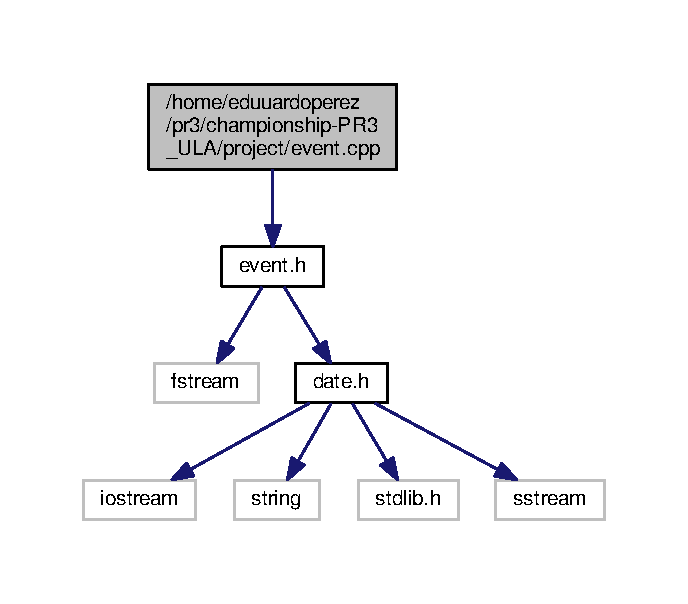
\includegraphics[width=330pt]{event_8cpp__incl}
\end{center}
\end{figure}
\subsection*{Funciones}
\begin{DoxyCompactItemize}
\item 
bool \hyperlink{event_8cpp_ae1b14fbe916bf72e371a0af9970530e0}{operator$<$} (const \hyperlink{class_event}{Event} \&event1, const \hyperlink{class_event}{Event} \&event2)
\begin{DoxyCompactList}\small\item\em operator $<$ \end{DoxyCompactList}\item 
bool \hyperlink{event_8cpp_aff3729450781b90f7710cf4647a05b98}{operator$>$} (const \hyperlink{class_event}{Event} \&event1, const \hyperlink{class_event}{Event} \&event2)
\begin{DoxyCompactList}\small\item\em operator $>$ \end{DoxyCompactList}\item 
ostream \& \hyperlink{event_8cpp_a91de7df4316bfc12fce6283858843121}{operator$<$$<$} (ostream \&event, const \hyperlink{class_event}{Event} \&e)
\begin{DoxyCompactList}\small\item\em operator $<$$<$ \end{DoxyCompactList}\item 
istream \& \hyperlink{event_8cpp_a7d68062f42bc7a2e68eef1767e4ea8ec}{operator$>$$>$} (istream \&event, \hyperlink{class_event}{Event} \&aux)
\begin{DoxyCompactList}\small\item\em operator $>$$>$ \end{DoxyCompactList}\item 
string \hyperlink{event_8cpp_aa36788e1fe302221cb9446e85b88155f}{Uint2\+String} (unsigned int num)
\begin{DoxyCompactList}\small\item\em Método Uint2\+String. \end{DoxyCompactList}\end{DoxyCompactItemize}


\subsection{Descripción detallada}
Implementación de la clase \hyperlink{class_event}{Event}. 

\begin{DoxyAuthor}{Autor}
Eduardo Perez (\href{mailto:edujpp1@gmail.com}{\tt edujpp1@gmail.\+com}) 
\end{DoxyAuthor}
\begin{DoxyVersion}{Versión}
1.\+0 
\end{DoxyVersion}
\begin{DoxyDate}{Fecha}
Noviembre, 2016 
\end{DoxyDate}


\subsection{Documentación de las funciones}
\index{event.\+cpp@{event.\+cpp}!operator$<$@{operator$<$}}
\index{operator$<$@{operator$<$}!event.\+cpp@{event.\+cpp}}
\subsubsection[{\texorpdfstring{operator$<$(const Event \&event1, const Event \&event2)}{operator<(const Event &event1, const Event &event2)}}]{\setlength{\rightskip}{0pt plus 5cm}bool operator$<$ (
\begin{DoxyParamCaption}
\item[{const {\bf Event} \&}]{, }
\item[{const {\bf Event} \&}]{}
\end{DoxyParamCaption}
)}\hypertarget{event_8cpp_ae1b14fbe916bf72e371a0af9970530e0}{}\label{event_8cpp_ae1b14fbe916bf72e371a0af9970530e0}


operator $<$ 

\begin{DoxyReturn}{Devuelve}
true si this es menor a event, false de lo contrario. 
\end{DoxyReturn}


Definición en la línea 168 del archivo event.\+cpp.

\index{event.\+cpp@{event.\+cpp}!operator$<$$<$@{operator$<$$<$}}
\index{operator$<$$<$@{operator$<$$<$}!event.\+cpp@{event.\+cpp}}
\subsubsection[{\texorpdfstring{operator$<$$<$(ostream \&event, const Event \&e)}{operator<<(ostream &event, const Event &e)}}]{\setlength{\rightskip}{0pt plus 5cm}ostream\& operator$<$$<$ (
\begin{DoxyParamCaption}
\item[{ostream \&}]{, }
\item[{const {\bf Event} \&}]{}
\end{DoxyParamCaption}
)}\hypertarget{event_8cpp_a91de7df4316bfc12fce6283858843121}{}\label{event_8cpp_a91de7df4316bfc12fce6283858843121}


operator $<$$<$ 

\begin{DoxyReturn}{Devuelve}
ostream\& event 
\end{DoxyReturn}


Definición en la línea 188 del archivo event.\+cpp.

\index{event.\+cpp@{event.\+cpp}!operator$>$@{operator$>$}}
\index{operator$>$@{operator$>$}!event.\+cpp@{event.\+cpp}}
\subsubsection[{\texorpdfstring{operator$>$(const Event \&event1, const Event \&event2)}{operator>(const Event &event1, const Event &event2)}}]{\setlength{\rightskip}{0pt plus 5cm}bool operator$>$ (
\begin{DoxyParamCaption}
\item[{const {\bf Event} \&}]{, }
\item[{const {\bf Event} \&}]{}
\end{DoxyParamCaption}
)}\hypertarget{event_8cpp_aff3729450781b90f7710cf4647a05b98}{}\label{event_8cpp_aff3729450781b90f7710cf4647a05b98}


operator $>$ 

\begin{DoxyReturn}{Devuelve}
true si this es mayor a event, false de lo contrario. 
\end{DoxyReturn}


Definición en la línea 178 del archivo event.\+cpp.

\index{event.\+cpp@{event.\+cpp}!operator$>$$>$@{operator$>$$>$}}
\index{operator$>$$>$@{operator$>$$>$}!event.\+cpp@{event.\+cpp}}
\subsubsection[{\texorpdfstring{operator$>$$>$(istream \&event, Event \&aux)}{operator>>(istream &event, Event &aux)}}]{\setlength{\rightskip}{0pt plus 5cm}istream\& operator$>$$>$ (
\begin{DoxyParamCaption}
\item[{istream \&}]{, }
\item[{{\bf Event} \&}]{}
\end{DoxyParamCaption}
)}\hypertarget{event_8cpp_a7d68062f42bc7a2e68eef1767e4ea8ec}{}\label{event_8cpp_a7d68062f42bc7a2e68eef1767e4ea8ec}


operator $>$$>$ 

\begin{DoxyReturn}{Devuelve}
istream\& event 
\end{DoxyReturn}


Definición en la línea 206 del archivo event.\+cpp.

\index{event.\+cpp@{event.\+cpp}!Uint2\+String@{Uint2\+String}}
\index{Uint2\+String@{Uint2\+String}!event.\+cpp@{event.\+cpp}}
\subsubsection[{\texorpdfstring{Uint2\+String(unsigned int num)}{Uint2String(unsigned int num)}}]{\setlength{\rightskip}{0pt plus 5cm}string Uint2\+String (
\begin{DoxyParamCaption}
\item[{unsigned}]{int}
\end{DoxyParamCaption}
)}\hypertarget{event_8cpp_aa36788e1fe302221cb9446e85b88155f}{}\label{event_8cpp_aa36788e1fe302221cb9446e85b88155f}


Método Uint2\+String. 

\begin{DoxyReturn}{Devuelve}
tipo int convertido a string 
\end{DoxyReturn}


Definición en la línea 281 del archivo event.\+cpp.


\hypertarget{event_8h}{}\section{Referencia del Archivo /home/eduuardoperez/pr3/championship-\/\+P\+R3\+\_\+\+U\+L\+A/project/event.h}
\label{event_8h}\index{/home/eduuardoperez/pr3/championship-\/\+P\+R3\+\_\+\+U\+L\+A/project/event.\+h@{/home/eduuardoperez/pr3/championship-\/\+P\+R3\+\_\+\+U\+L\+A/project/event.\+h}}


Clase \hyperlink{class_event}{Event}.  


{\ttfamily \#include $<$fstream$>$}\\*
{\ttfamily \#include \char`\"{}date.\+h\char`\"{}}\\*
Dependencia gráfica adjunta para event.\+h\+:\nopagebreak
\begin{figure}[H]
\begin{center}
\leavevmode
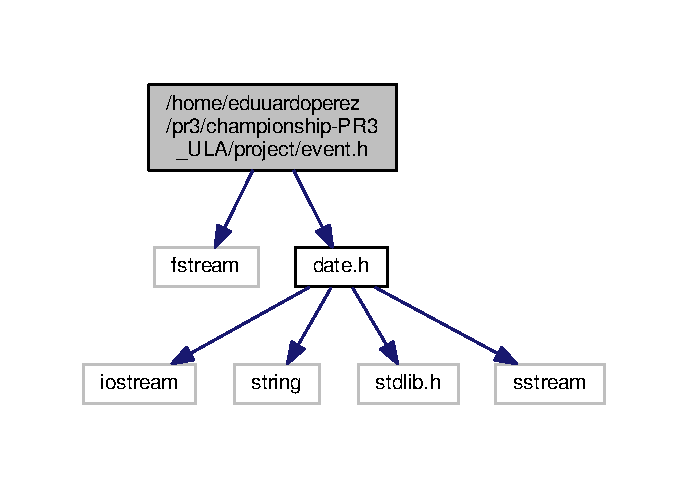
\includegraphics[width=330pt]{event_8h__incl}
\end{center}
\end{figure}
Gráfico de los archivos que directa o indirectamente incluyen a este archivo\+:\nopagebreak
\begin{figure}[H]
\begin{center}
\leavevmode
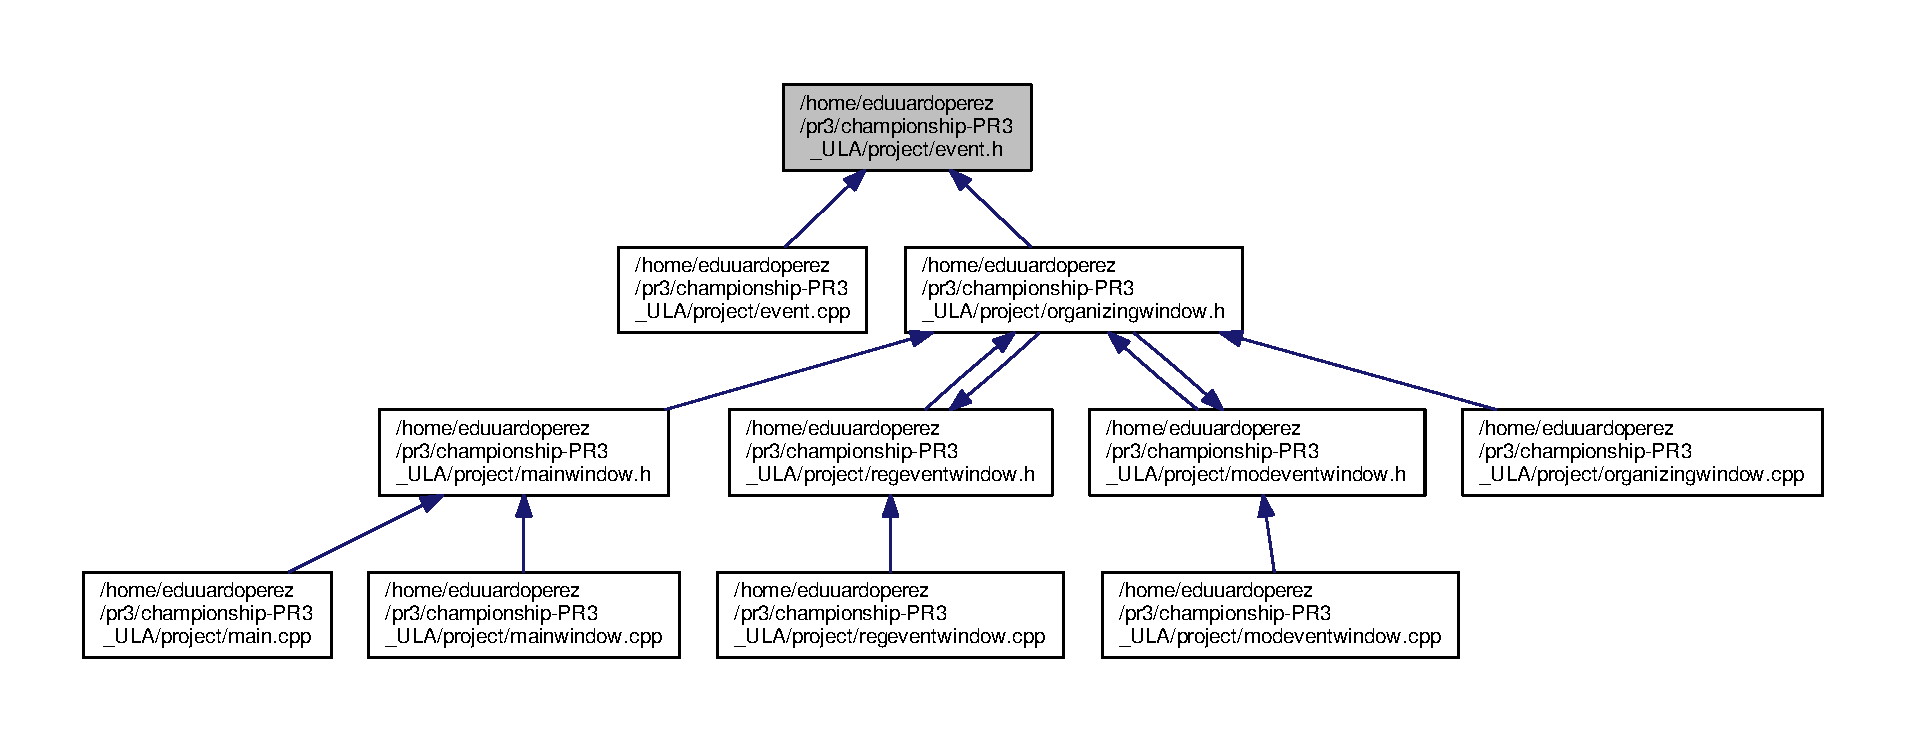
\includegraphics[width=350pt]{event_8h__dep__incl}
\end{center}
\end{figure}
\subsection*{Estructuras de datos}
\begin{DoxyCompactItemize}
\item 
class \hyperlink{class_event}{Event}
\begin{DoxyCompactList}\small\item\em Clase \hyperlink{class_event}{Event}. \end{DoxyCompactList}\end{DoxyCompactItemize}
\subsection*{Funciones}
\begin{DoxyCompactItemize}
\item 
bool \hyperlink{event_8h_a83ed973c897fce04b33595c56342bc1c}{operator$<$} (const \hyperlink{class_event}{Event} \&, const \hyperlink{class_event}{Event} \&)
\begin{DoxyCompactList}\small\item\em operator $<$ \end{DoxyCompactList}\item 
bool \hyperlink{event_8h_a6be60f4389af6836f677f3ec902a5da7}{operator$>$} (const \hyperlink{class_event}{Event} \&, const \hyperlink{class_event}{Event} \&)
\begin{DoxyCompactList}\small\item\em operator $>$ \end{DoxyCompactList}\item 
ostream \& \hyperlink{event_8h_ae89bc187e03d6768c657ffff9c3c040c}{operator$<$$<$} (ostream \&, const \hyperlink{class_event}{Event} \&)
\begin{DoxyCompactList}\small\item\em operator $<$$<$ \end{DoxyCompactList}\item 
istream \& \hyperlink{event_8h_a6e09cc4670fbfa33a6d31704e3ad5508}{operator$>$$>$} (istream \&, \hyperlink{class_event}{Event} \&)
\begin{DoxyCompactList}\small\item\em operator $>$$>$ \end{DoxyCompactList}\end{DoxyCompactItemize}


\subsection{Descripción detallada}
Clase \hyperlink{class_event}{Event}. 

\begin{DoxyAuthor}{Autor}
Eduardo Perez (\href{mailto:edujpp1@gmail.com}{\tt edujpp1@gmail.\+com}) 
\end{DoxyAuthor}
\begin{DoxyVersion}{Versión}
1.\+0 
\end{DoxyVersion}
\begin{DoxyDate}{Fecha}
Noviembre, 2016 
\end{DoxyDate}


\subsection{Documentación de las funciones}
\index{event.\+h@{event.\+h}!operator$<$@{operator$<$}}
\index{operator$<$@{operator$<$}!event.\+h@{event.\+h}}
\subsubsection[{\texorpdfstring{operator$<$(const Event \&, const Event \&)}{operator<(const Event &, const Event &)}}]{\setlength{\rightskip}{0pt plus 5cm}bool operator$<$ (
\begin{DoxyParamCaption}
\item[{const {\bf Event} \&}]{, }
\item[{const {\bf Event} \&}]{}
\end{DoxyParamCaption}
)}\hypertarget{event_8h_a83ed973c897fce04b33595c56342bc1c}{}\label{event_8h_a83ed973c897fce04b33595c56342bc1c}


operator $<$ 

\begin{DoxyReturn}{Devuelve}
true si this es menor a event, false de lo contrario. 
\end{DoxyReturn}


Definición en la línea 168 del archivo event.\+cpp.

\index{event.\+h@{event.\+h}!operator$<$$<$@{operator$<$$<$}}
\index{operator$<$$<$@{operator$<$$<$}!event.\+h@{event.\+h}}
\subsubsection[{\texorpdfstring{operator$<$$<$(ostream \&, const Event \&)}{operator<<(ostream &, const Event &)}}]{\setlength{\rightskip}{0pt plus 5cm}ostream\& operator$<$$<$ (
\begin{DoxyParamCaption}
\item[{ostream \&}]{, }
\item[{const {\bf Event} \&}]{}
\end{DoxyParamCaption}
)}\hypertarget{event_8h_ae89bc187e03d6768c657ffff9c3c040c}{}\label{event_8h_ae89bc187e03d6768c657ffff9c3c040c}


operator $<$$<$ 

\begin{DoxyReturn}{Devuelve}
ostream\& event 
\end{DoxyReturn}


Definición en la línea 188 del archivo event.\+cpp.

\index{event.\+h@{event.\+h}!operator$>$@{operator$>$}}
\index{operator$>$@{operator$>$}!event.\+h@{event.\+h}}
\subsubsection[{\texorpdfstring{operator$>$(const Event \&, const Event \&)}{operator>(const Event &, const Event &)}}]{\setlength{\rightskip}{0pt plus 5cm}bool operator$>$ (
\begin{DoxyParamCaption}
\item[{const {\bf Event} \&}]{, }
\item[{const {\bf Event} \&}]{}
\end{DoxyParamCaption}
)}\hypertarget{event_8h_a6be60f4389af6836f677f3ec902a5da7}{}\label{event_8h_a6be60f4389af6836f677f3ec902a5da7}


operator $>$ 

\begin{DoxyReturn}{Devuelve}
true si this es mayor a event, false de lo contrario. 
\end{DoxyReturn}


Definición en la línea 178 del archivo event.\+cpp.

\index{event.\+h@{event.\+h}!operator$>$$>$@{operator$>$$>$}}
\index{operator$>$$>$@{operator$>$$>$}!event.\+h@{event.\+h}}
\subsubsection[{\texorpdfstring{operator$>$$>$(istream \&, Event \&)}{operator>>(istream &, Event &)}}]{\setlength{\rightskip}{0pt plus 5cm}istream\& operator$>$$>$ (
\begin{DoxyParamCaption}
\item[{istream \&}]{, }
\item[{{\bf Event} \&}]{}
\end{DoxyParamCaption}
)}\hypertarget{event_8h_a6e09cc4670fbfa33a6d31704e3ad5508}{}\label{event_8h_a6e09cc4670fbfa33a6d31704e3ad5508}


operator $>$$>$ 

\begin{DoxyReturn}{Devuelve}
istream\& event 
\end{DoxyReturn}


Definición en la línea 206 del archivo event.\+cpp.


\hypertarget{mainwindow_8cpp}{}\section{Referencia del Archivo /home/eduuardoperez/pr3/championship-\/\+P\+R3\+\_\+\+U\+L\+A/project/mainwindow.cpp}
\label{mainwindow_8cpp}\index{/home/eduuardoperez/pr3/championship-\/\+P\+R3\+\_\+\+U\+L\+A/project/mainwindow.\+cpp@{/home/eduuardoperez/pr3/championship-\/\+P\+R3\+\_\+\+U\+L\+A/project/mainwindow.\+cpp}}


Implementación de la clase \hyperlink{class_main_window}{Main\+Window}.  


{\ttfamily \#include \char`\"{}mainwindow.\+h\char`\"{}}\\*
{\ttfamily \#include \char`\"{}ui\+\_\+mainwindow.\+h\char`\"{}}\\*
Dependencia gráfica adjunta para mainwindow.\+cpp\+:\nopagebreak
\begin{figure}[H]
\begin{center}
\leavevmode
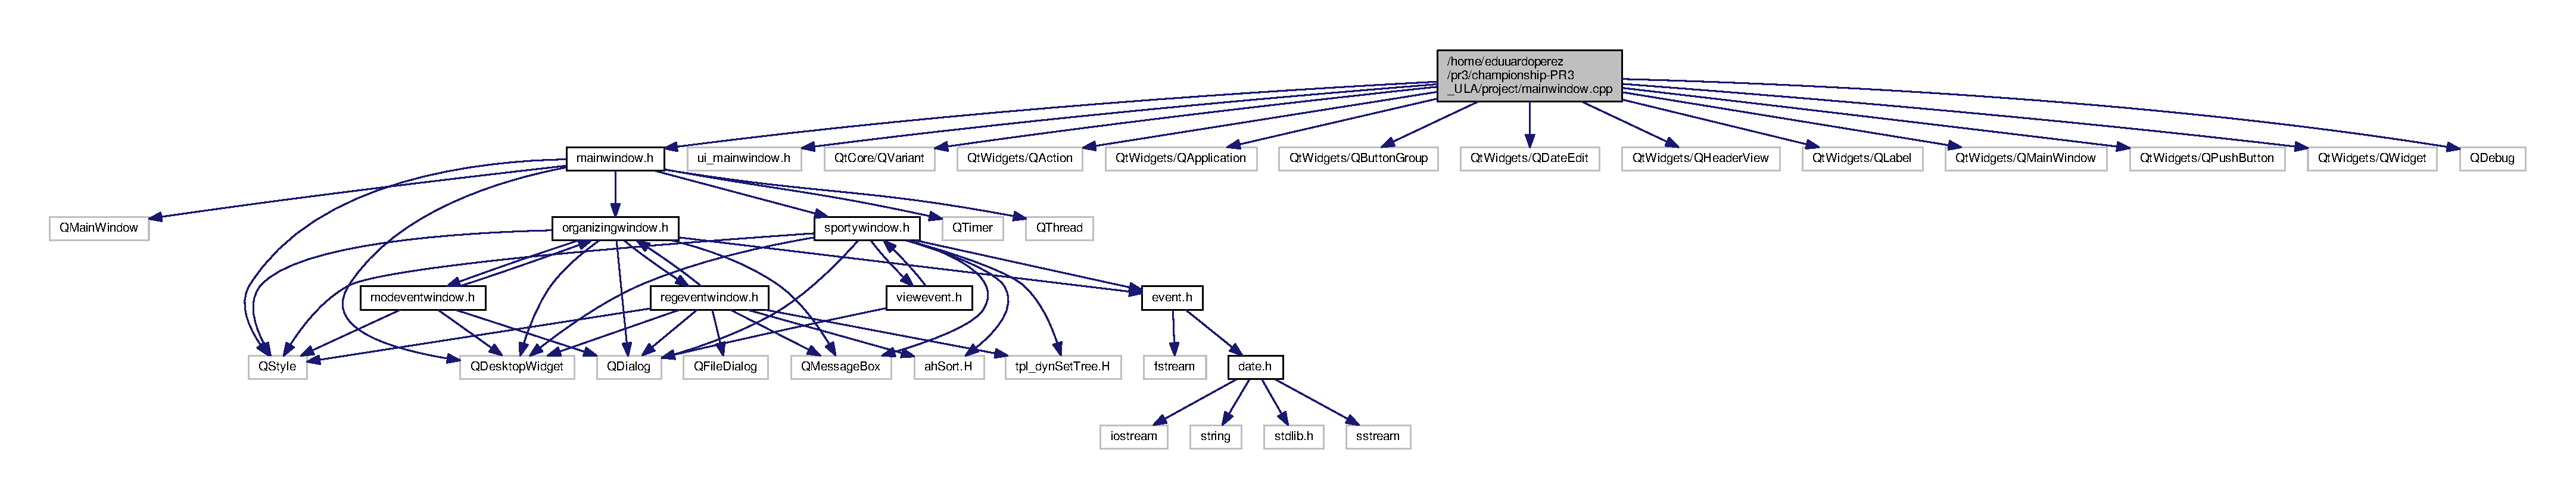
\includegraphics[width=350pt]{mainwindow_8cpp__incl}
\end{center}
\end{figure}
\subsection*{Funciones}
\begin{DoxyCompactItemize}
\item 
bool \hyperlink{mainwindow_8cpp_a527663192ac76098ca0779fb684c1585}{is\+\_\+empty\+File} (ifstream \&file)
\begin{DoxyCompactList}\small\item\em Método is\+\_\+empty\+File. \end{DoxyCompactList}\end{DoxyCompactItemize}


\subsection{Descripción detallada}
Implementación de la clase \hyperlink{class_main_window}{Main\+Window}. 

\begin{DoxyAuthor}{Autor}
Eduardo Perez (\href{mailto:edujpp1@gmail.com}{\tt edujpp1@gmail.\+com}) 
\end{DoxyAuthor}
\begin{DoxyVersion}{Versión}
1.\+0 
\end{DoxyVersion}
\begin{DoxyDate}{Fecha}
Noviembre, 2016 
\end{DoxyDate}


\subsection{Documentación de las funciones}
\index{mainwindow.\+cpp@{mainwindow.\+cpp}!is\+\_\+empty\+File@{is\+\_\+empty\+File}}
\index{is\+\_\+empty\+File@{is\+\_\+empty\+File}!mainwindow.\+cpp@{mainwindow.\+cpp}}
\subsubsection[{\texorpdfstring{is\+\_\+empty\+File(ifstream \&file)}{is_emptyFile(ifstream &file)}}]{\setlength{\rightskip}{0pt plus 5cm}bool is\+\_\+empty\+File (
\begin{DoxyParamCaption}
\item[{ifstream \&}]{}
\end{DoxyParamCaption}
)}\hypertarget{mainwindow_8cpp_a527663192ac76098ca0779fb684c1585}{}\label{mainwindow_8cpp_a527663192ac76098ca0779fb684c1585}


Método is\+\_\+empty\+File. 

\begin{DoxyReturn}{Devuelve}
true si file esta vacio, false de lo contrario 
\end{DoxyReturn}


Definición en la línea 139 del archivo mainwindow.\+cpp.


\hypertarget{mainwindow_8h}{}\section{Referencia del Archivo /home/eduuardoperez/pr3/championship/project/mainwindow.h}
\label{mainwindow_8h}\index{/home/eduuardoperez/pr3/championship/project/mainwindow.\+h@{/home/eduuardoperez/pr3/championship/project/mainwindow.\+h}}


Clase \hyperlink{class_main_window}{Main\+Window}.  


{\ttfamily \#include $<$Q\+Main\+Window$>$}\\*
Dependencia gráfica adjunta para mainwindow.\+h\+:
% FIG 0
Gráfico de los archivos que directa o indirectamente incluyen a este archivo\+:
% FIG 1
\subsection*{Estructuras de datos}
\begin{DoxyCompactItemize}
\item 
class \hyperlink{class_main_window}{Main\+Window}
\begin{DoxyCompactList}\small\item\em Clase \hyperlink{class_main_window}{Main\+Window}. \end{DoxyCompactList}\end{DoxyCompactItemize}


\subsection{Descripción detallada}
Clase \hyperlink{class_main_window}{Main\+Window}. 

\begin{DoxyAuthor}{Autor}
Eduardo Perez (\href{mailto:edujpp1@gmail.com}{\tt edujpp1@gmail.\+com}) 

Angely Azuaje (\href{mailto:angiibri4@gmail.com}{\tt angiibri4@gmail.\+com}) 
\end{DoxyAuthor}
\begin{DoxyVersion}{Versión}
1.\+0 
\end{DoxyVersion}
\begin{DoxyDate}{Fecha}
Noviembre, 2016 
\end{DoxyDate}

\hypertarget{modeventwindow_8cpp}{}\section{Referencia del Archivo /home/eduuardoperez/pr3/championship-\/\+P\+R3\+\_\+\+U\+L\+A/project/modeventwindow.cpp}
\label{modeventwindow_8cpp}\index{/home/eduuardoperez/pr3/championship-\/\+P\+R3\+\_\+\+U\+L\+A/project/modeventwindow.\+cpp@{/home/eduuardoperez/pr3/championship-\/\+P\+R3\+\_\+\+U\+L\+A/project/modeventwindow.\+cpp}}


Implementación de la clase \hyperlink{class_mod_event_window}{Mod\+Event\+Window}.  


{\ttfamily \#include \char`\"{}modeventwindow.\+h\char`\"{}}\\*
{\ttfamily \#include \char`\"{}ui\+\_\+modeventwindow.\+h\char`\"{}}\\*
Dependencia gráfica adjunta para modeventwindow.\+cpp\+:\nopagebreak
\begin{figure}[H]
\begin{center}
\leavevmode
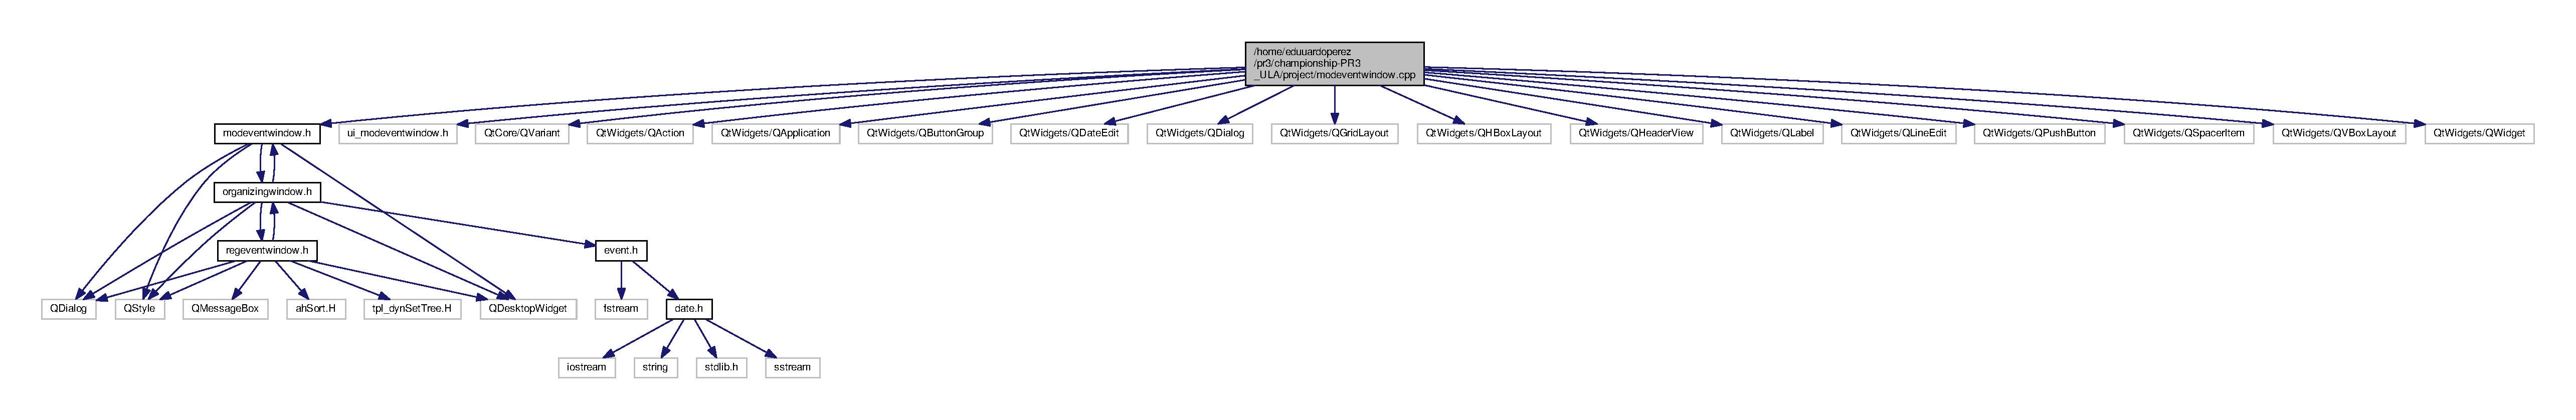
\includegraphics[width=350pt]{modeventwindow_8cpp__incl}
\end{center}
\end{figure}


\subsection{Descripción detallada}
Implementación de la clase \hyperlink{class_mod_event_window}{Mod\+Event\+Window}. 

\begin{DoxyAuthor}{Autor}
Eduardo Perez (\href{mailto:edujpp1@gmail.com}{\tt edujpp1@gmail.\+com}) 
\end{DoxyAuthor}
\begin{DoxyVersion}{Versión}
1.\+0 
\end{DoxyVersion}
\begin{DoxyDate}{Fecha}
Noviembre, 2016 
\end{DoxyDate}

\hypertarget{modeventwindow_8h}{}\section{Referencia del Archivo /home/eduuardoperez/pr3/championship-\/\+P\+R3\+\_\+\+U\+L\+A/project/modeventwindow.h}
\label{modeventwindow_8h}\index{/home/eduuardoperez/pr3/championship-\/\+P\+R3\+\_\+\+U\+L\+A/project/modeventwindow.\+h@{/home/eduuardoperez/pr3/championship-\/\+P\+R3\+\_\+\+U\+L\+A/project/modeventwindow.\+h}}


Clase \hyperlink{class_mod_event_window}{Mod\+Event\+Window}.  


{\ttfamily \#include $<$Q\+Dialog$>$}\\*
{\ttfamily \#include $<$Q\+Style$>$}\\*
{\ttfamily \#include $<$Q\+Desktop\+Widget$>$}\\*
{\ttfamily \#include \char`\"{}organizingwindow.\+h\char`\"{}}\\*
Dependencia gráfica adjunta para modeventwindow.\+h\+:\nopagebreak
\begin{figure}[H]
\begin{center}
\leavevmode
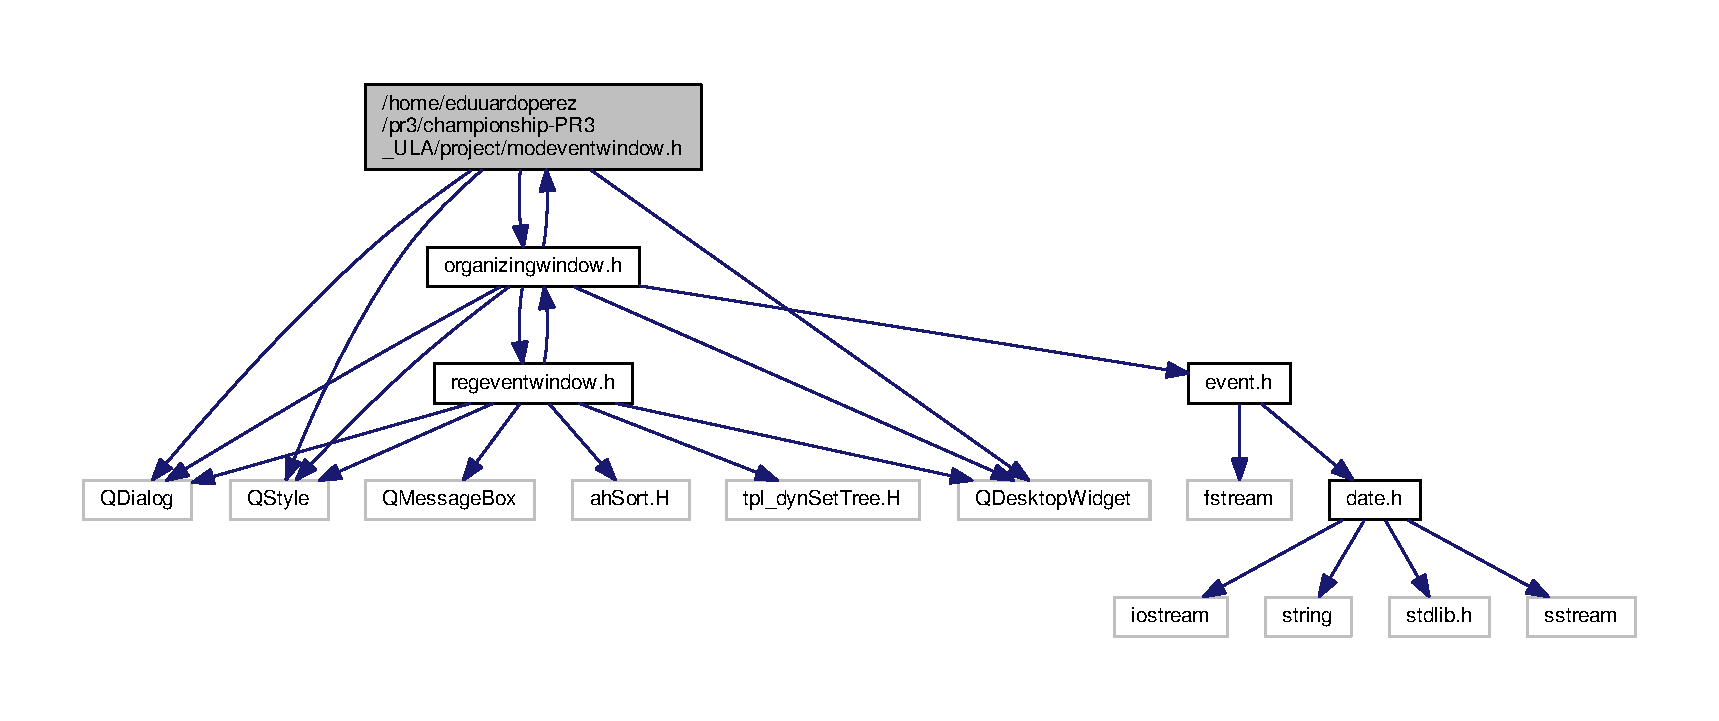
\includegraphics[width=350pt]{modeventwindow_8h__incl}
\end{center}
\end{figure}
Gráfico de los archivos que directa o indirectamente incluyen a este archivo\+:\nopagebreak
\begin{figure}[H]
\begin{center}
\leavevmode
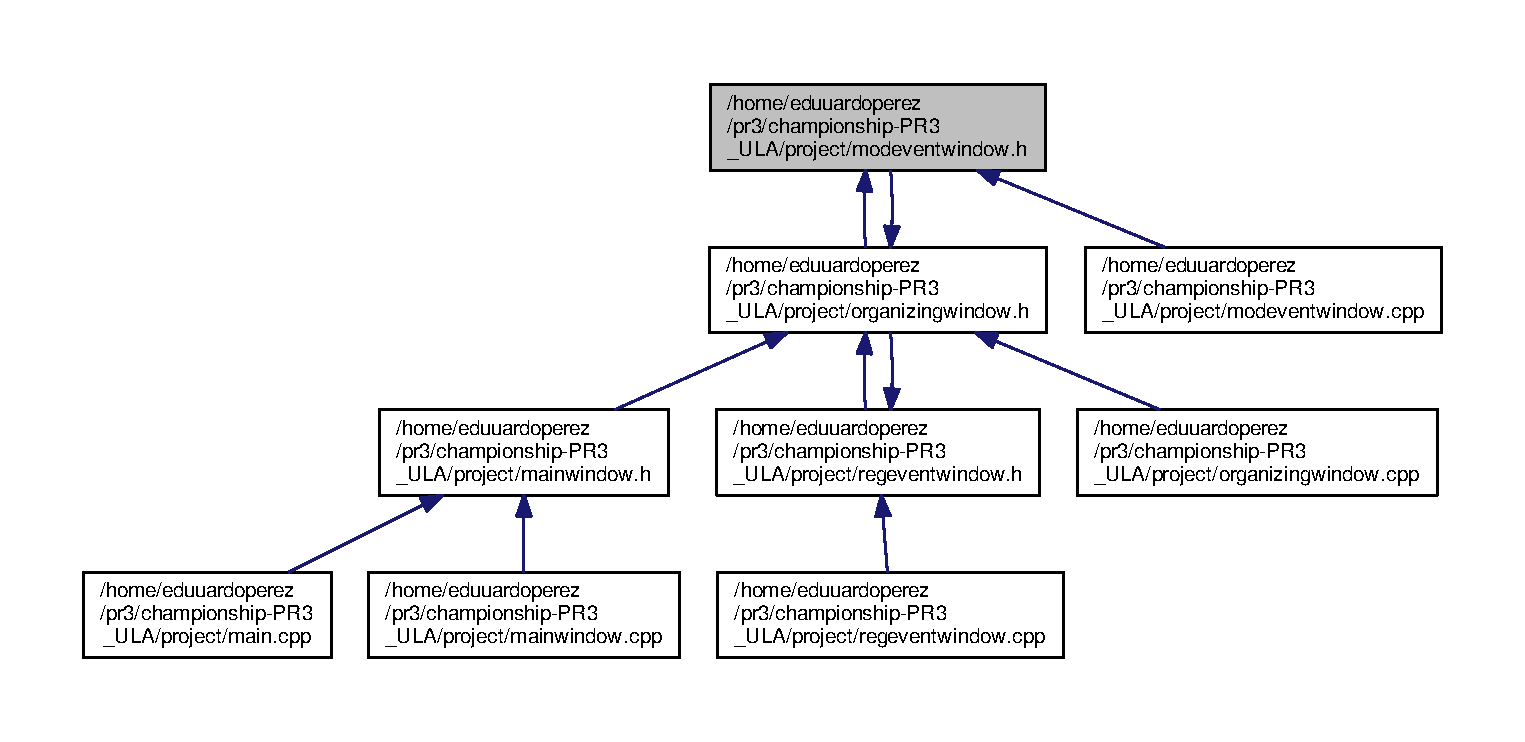
\includegraphics[width=350pt]{modeventwindow_8h__dep__incl}
\end{center}
\end{figure}
\subsection*{Estructuras de datos}
\begin{DoxyCompactItemize}
\item 
class \hyperlink{class_mod_event_window}{Mod\+Event\+Window}
\begin{DoxyCompactList}\small\item\em Clase \hyperlink{class_mod_event_window}{Mod\+Event\+Window}. \end{DoxyCompactList}\end{DoxyCompactItemize}


\subsection{Descripción detallada}
Clase \hyperlink{class_mod_event_window}{Mod\+Event\+Window}. 

\begin{DoxyAuthor}{Autor}
Eduardo Perez (\href{mailto:edujpp1@gmail.com}{\tt edujpp1@gmail.\+com}) 
\end{DoxyAuthor}
\begin{DoxyVersion}{Versión}
1.\+0 
\end{DoxyVersion}
\begin{DoxyDate}{Fecha}
Noviembre, 2016 
\end{DoxyDate}

\hypertarget{organizingwindow_8cpp}{}\section{Referencia del Archivo /home/eduuardoperez/pr3/championship-\/\+P\+R3\+\_\+\+U\+L\+A/project/organizingwindow.cpp}
\label{organizingwindow_8cpp}\index{/home/eduuardoperez/pr3/championship-\/\+P\+R3\+\_\+\+U\+L\+A/project/organizingwindow.\+cpp@{/home/eduuardoperez/pr3/championship-\/\+P\+R3\+\_\+\+U\+L\+A/project/organizingwindow.\+cpp}}


Implementación de la clase \hyperlink{class_organizing_window}{Organizing\+Window}.  


{\ttfamily \#include \char`\"{}organizingwindow.\+h\char`\"{}}\\*
{\ttfamily \#include \char`\"{}ui\+\_\+organizingwindow.\+h\char`\"{}}\\*
Dependencia gráfica adjunta para organizingwindow.\+cpp\+:\nopagebreak
\begin{figure}[H]
\begin{center}
\leavevmode
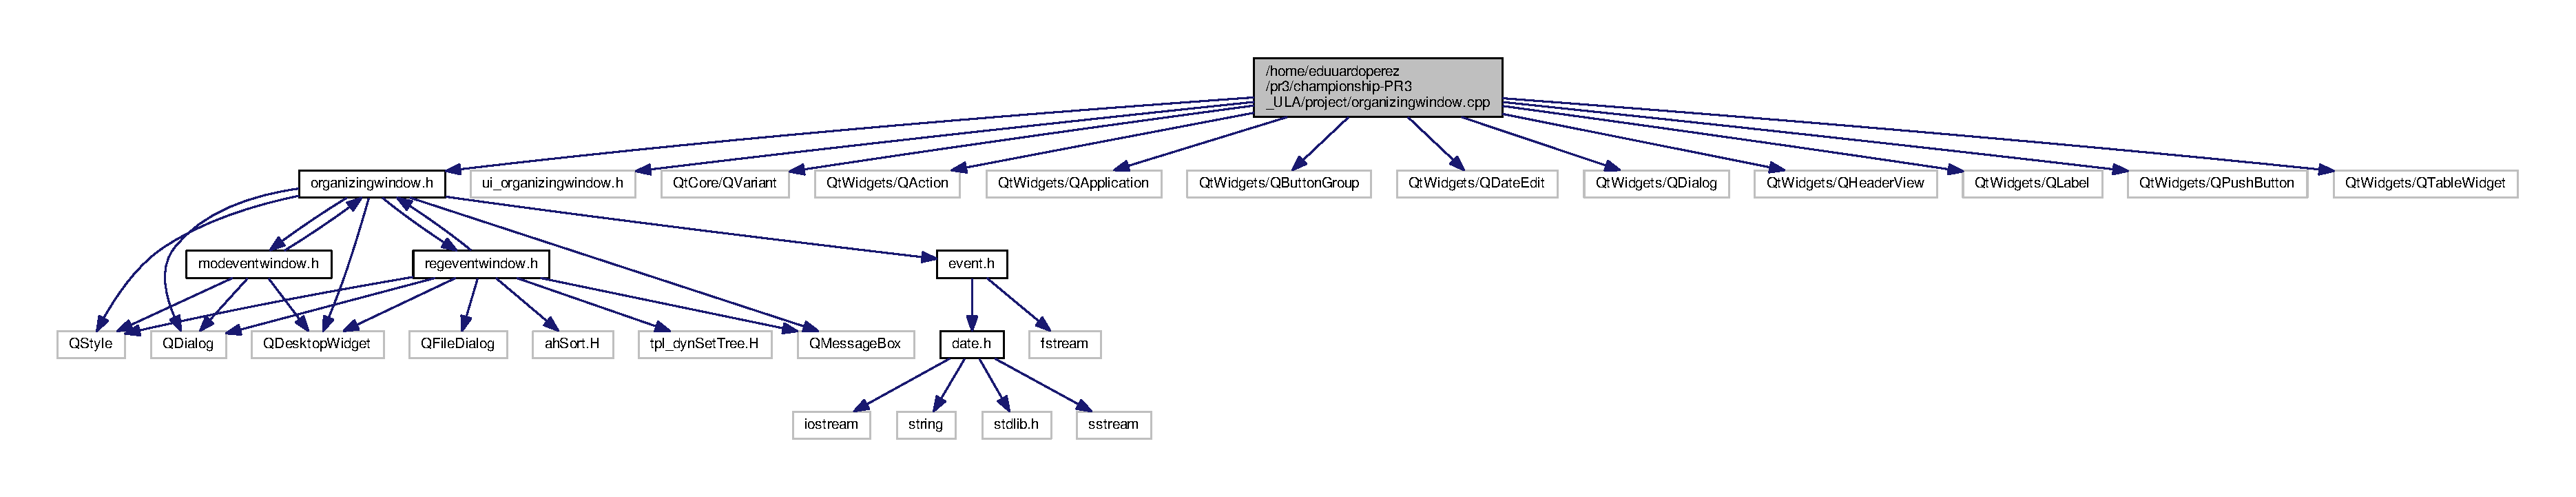
\includegraphics[width=350pt]{organizingwindow_8cpp__incl}
\end{center}
\end{figure}


\subsection{Descripción detallada}
Implementación de la clase \hyperlink{class_organizing_window}{Organizing\+Window}. 

\begin{DoxyAuthor}{Autor}
Eduardo Perez (\href{mailto:edujpp1@gmail.com}{\tt edujpp1@gmail.\+com}) 
\end{DoxyAuthor}
\begin{DoxyVersion}{Versión}
1.\+0 
\end{DoxyVersion}
\begin{DoxyDate}{Fecha}
Noviembre, 2016 
\end{DoxyDate}

\hypertarget{organizingwindow_8h}{}\section{Referencia del Archivo /home/eduuardoperez/pr3/championship-\/\+P\+R3\+\_\+\+U\+L\+A/project/organizingwindow.h}
\label{organizingwindow_8h}\index{/home/eduuardoperez/pr3/championship-\/\+P\+R3\+\_\+\+U\+L\+A/project/organizingwindow.\+h@{/home/eduuardoperez/pr3/championship-\/\+P\+R3\+\_\+\+U\+L\+A/project/organizingwindow.\+h}}


Clase \hyperlink{class_organizing_window}{Organizing\+Window}.  


{\ttfamily \#include $<$Q\+Dialog$>$}\\*
{\ttfamily \#include $<$Q\+Style$>$}\\*
{\ttfamily \#include $<$Q\+Desktop\+Widget$>$}\\*
{\ttfamily \#include \char`\"{}event.\+h\char`\"{}}\\*
{\ttfamily \#include \char`\"{}regeventwindow.\+h\char`\"{}}\\*
Dependencia gráfica adjunta para organizingwindow.\+h\+:\nopagebreak
\begin{figure}[H]
\begin{center}
\leavevmode
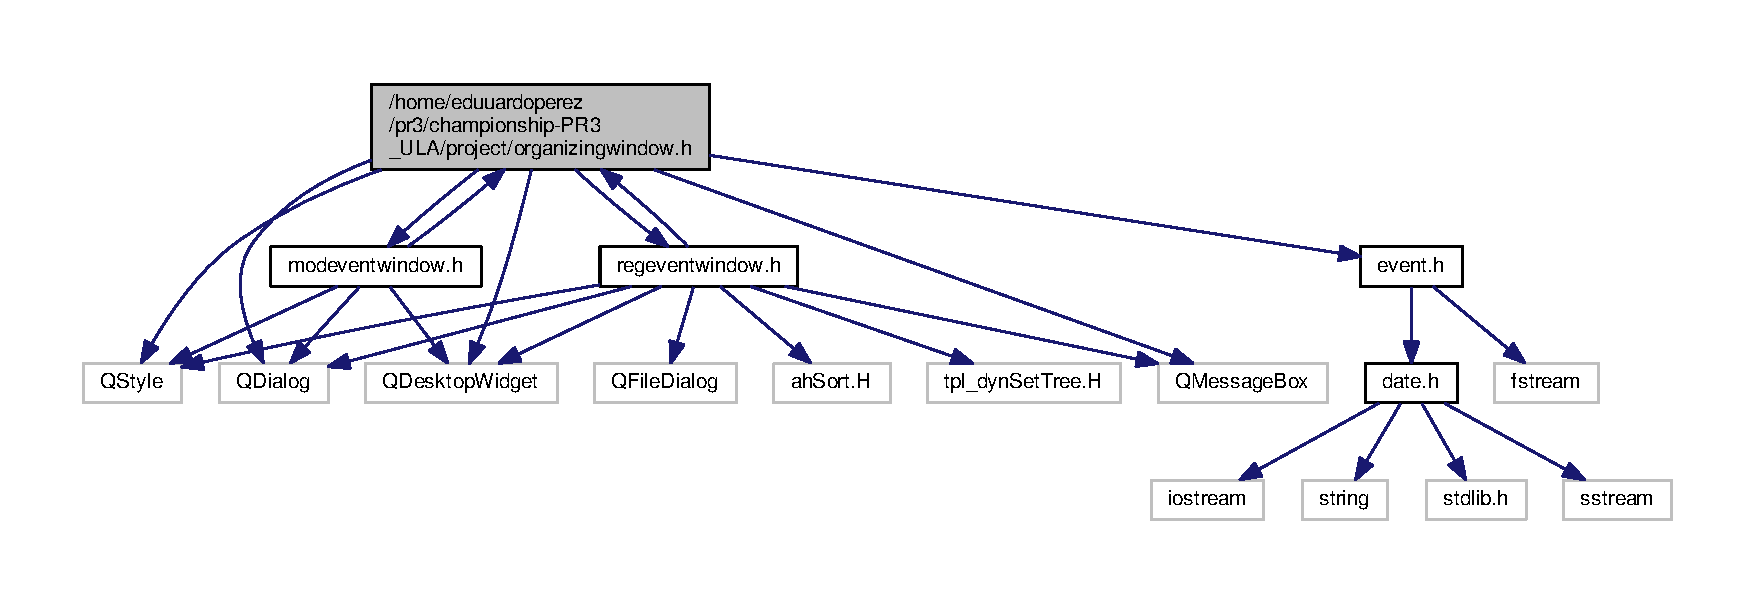
\includegraphics[width=350pt]{organizingwindow_8h__incl}
\end{center}
\end{figure}
Gráfico de los archivos que directa o indirectamente incluyen a este archivo\+:\nopagebreak
\begin{figure}[H]
\begin{center}
\leavevmode
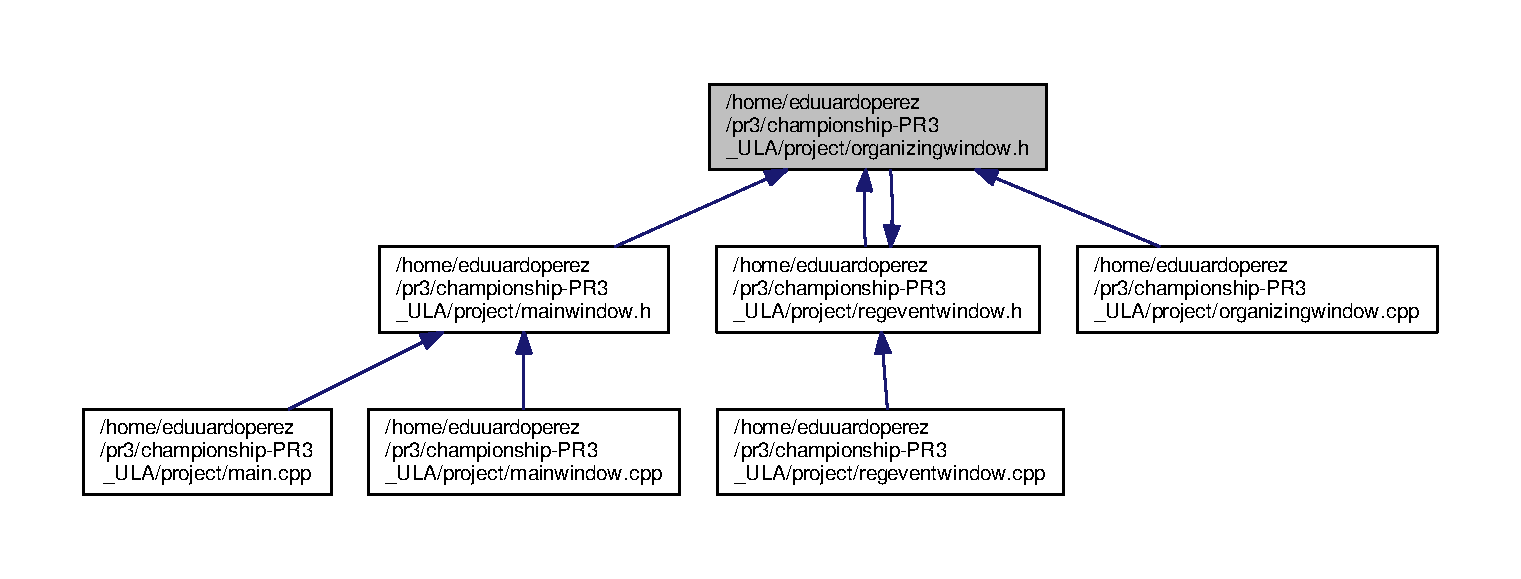
\includegraphics[width=350pt]{organizingwindow_8h__dep__incl}
\end{center}
\end{figure}
\subsection*{Estructuras de datos}
\begin{DoxyCompactItemize}
\item 
class \hyperlink{class_organizing_window}{Organizing\+Window}
\begin{DoxyCompactList}\small\item\em Clase \hyperlink{class_organizing_window}{Organizing\+Window}. \end{DoxyCompactList}\end{DoxyCompactItemize}


\subsection{Descripción detallada}
Clase \hyperlink{class_organizing_window}{Organizing\+Window}. 

\begin{DoxyAuthor}{Autor}
Eduardo Perez (\href{mailto:edujpp1@gmail.com}{\tt edujpp1@gmail.\+com}) 
\end{DoxyAuthor}
\begin{DoxyVersion}{Versión}
1.\+0 
\end{DoxyVersion}
\begin{DoxyDate}{Fecha}
Noviembre, 2016 
\end{DoxyDate}

\hypertarget{participant_8cpp}{}\section{Referencia del Archivo /home/eduuardoperez/pr3/championship-\/\+P\+R3\+\_\+\+U\+L\+A/project/participant.cpp}
\label{participant_8cpp}\index{/home/eduuardoperez/pr3/championship-\/\+P\+R3\+\_\+\+U\+L\+A/project/participant.\+cpp@{/home/eduuardoperez/pr3/championship-\/\+P\+R3\+\_\+\+U\+L\+A/project/participant.\+cpp}}


Implementación de la clase \hyperlink{class_participant}{Participant}.  


{\ttfamily \#include \char`\"{}participant.\+h\char`\"{}}\\*
Dependencia gráfica adjunta para participant.\+cpp\+:\nopagebreak
\begin{figure}[H]
\begin{center}
\leavevmode
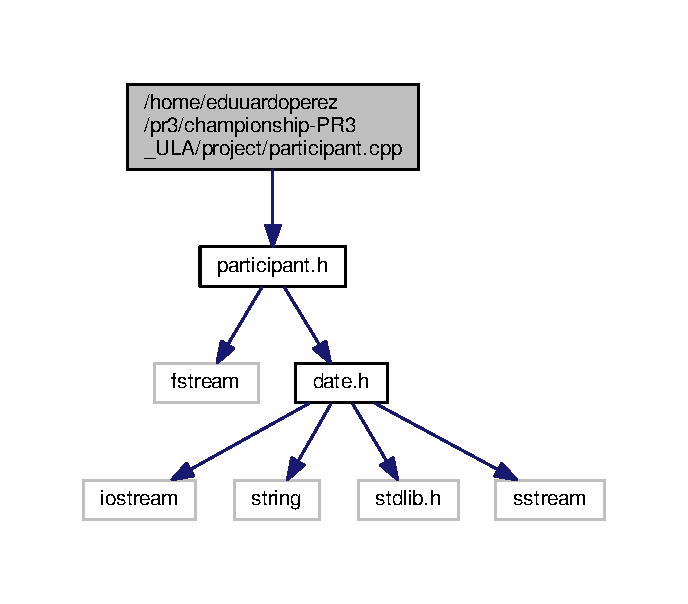
\includegraphics[width=330pt]{participant_8cpp__incl}
\end{center}
\end{figure}
\subsection*{Funciones}
\begin{DoxyCompactItemize}
\item 
int \hyperlink{participant_8cpp_a4deb5935b4c161b878a63e795b4d8427}{operator$<$} (const \hyperlink{class_participant}{Participant} \&p1, const \hyperlink{class_participant}{Participant} \&p2)
\begin{DoxyCompactList}\small\item\em operator $<$ \end{DoxyCompactList}\item 
ostream \& \hyperlink{participant_8cpp_a4b5d7073823a6d7f530b2449f5318b86}{operator$<$$<$} (ostream \&participant, const \hyperlink{class_participant}{Participant} \&p)
\begin{DoxyCompactList}\small\item\em operator $<$$<$ \end{DoxyCompactList}\item 
istream \& \hyperlink{participant_8cpp_a9defb1b815d27cfb3e6322dbcb4a44ff}{operator$>$$>$} (istream \&participant, \hyperlink{class_participant}{Participant} \&aux)
\begin{DoxyCompactList}\small\item\em operator $>$$>$ \end{DoxyCompactList}\item 
unsigned int \hyperlink{participant_8cpp_a588b505c3456212aefeb7b854b50c0a8}{calculate\+Age} (unsigned int born\+Day, unsigned int born\+Month, unsigned int born\+Year, unsigned int curr\+Day, unsigned int curr\+Month, unsigned int curr\+Year)
\begin{DoxyCompactList}\small\item\em calculate\+Age \end{DoxyCompactList}\end{DoxyCompactItemize}


\subsection{Descripción detallada}
Implementación de la clase \hyperlink{class_participant}{Participant}. 

\begin{DoxyAuthor}{Autor}
Eduardo Perez (\href{mailto:edujpp1@gmail.com}{\tt edujpp1@gmail.\+com}) 
\end{DoxyAuthor}
\begin{DoxyVersion}{Versión}
1.\+0 
\end{DoxyVersion}
\begin{DoxyDate}{Fecha}
Noviembre, 2016 
\end{DoxyDate}


\subsection{Documentación de las funciones}
\index{participant.\+cpp@{participant.\+cpp}!calculate\+Age@{calculate\+Age}}
\index{calculate\+Age@{calculate\+Age}!participant.\+cpp@{participant.\+cpp}}
\subsubsection[{\texorpdfstring{calculate\+Age(unsigned int born\+Day, unsigned int born\+Month, unsigned int born\+Year, unsigned int curr\+Day, unsigned int curr\+Month, unsigned int curr\+Year)}{calculateAge(unsigned int bornDay, unsigned int bornMonth, unsigned int bornYear, unsigned int currDay, unsigned int currMonth, unsigned int currYear)}}]{\setlength{\rightskip}{0pt plus 5cm}unsigned int calculate\+Age (
\begin{DoxyParamCaption}
\item[{unsigned}]{int, }
\item[{unsigned}]{int, }
\item[{unsigned}]{int, }
\item[{unsigned}]{int, }
\item[{unsigned}]{int, }
\item[{unsigned}]{int}
\end{DoxyParamCaption}
)}\hypertarget{participant_8cpp_a588b505c3456212aefeb7b854b50c0a8}{}\label{participant_8cpp_a588b505c3456212aefeb7b854b50c0a8}


calculate\+Age 

\begin{DoxyReturn}{Devuelve}
Años comprendidos entre dos fechas, 0 si se ingresan fechas erróneas. 
\end{DoxyReturn}


Definición en la línea 184 del archivo participant.\+cpp.

\index{participant.\+cpp@{participant.\+cpp}!operator$<$@{operator$<$}}
\index{operator$<$@{operator$<$}!participant.\+cpp@{participant.\+cpp}}
\subsubsection[{\texorpdfstring{operator$<$(const Participant \&p1, const Participant \&p2)}{operator<(const Participant &p1, const Participant &p2)}}]{\setlength{\rightskip}{0pt plus 5cm}int operator$<$ (
\begin{DoxyParamCaption}
\item[{const {\bf Participant} \&}]{, }
\item[{const {\bf Participant} \&}]{}
\end{DoxyParamCaption}
)}\hypertarget{participant_8cpp_a4deb5935b4c161b878a63e795b4d8427}{}\label{participant_8cpp_a4deb5935b4c161b878a63e795b4d8427}


operator $<$ 

\begin{DoxyReturn}{Devuelve}
1 si this es menor a event, 0 si no lo es. 
\end{DoxyReturn}


Definición en la línea 116 del archivo participant.\+cpp.

\index{participant.\+cpp@{participant.\+cpp}!operator$<$$<$@{operator$<$$<$}}
\index{operator$<$$<$@{operator$<$$<$}!participant.\+cpp@{participant.\+cpp}}
\subsubsection[{\texorpdfstring{operator$<$$<$(ostream \&participant, const Participant \&p)}{operator<<(ostream &participant, const Participant &p)}}]{\setlength{\rightskip}{0pt plus 5cm}ostream\& operator$<$$<$ (
\begin{DoxyParamCaption}
\item[{ostream \&}]{, }
\item[{const {\bf Participant} \&}]{}
\end{DoxyParamCaption}
)}\hypertarget{participant_8cpp_a4b5d7073823a6d7f530b2449f5318b86}{}\label{participant_8cpp_a4b5d7073823a6d7f530b2449f5318b86}


operator $<$$<$ 

\begin{DoxyReturn}{Devuelve}
ostream\& participant 
\end{DoxyReturn}


Definición en la línea 123 del archivo participant.\+cpp.

\index{participant.\+cpp@{participant.\+cpp}!operator$>$$>$@{operator$>$$>$}}
\index{operator$>$$>$@{operator$>$$>$}!participant.\+cpp@{participant.\+cpp}}
\subsubsection[{\texorpdfstring{operator$>$$>$(istream \&participant, Participant \&aux)}{operator>>(istream &participant, Participant &aux)}}]{\setlength{\rightskip}{0pt plus 5cm}istream\& operator$>$$>$ (
\begin{DoxyParamCaption}
\item[{istream \&}]{, }
\item[{{\bf Participant} \&}]{}
\end{DoxyParamCaption}
)}\hypertarget{participant_8cpp_a9defb1b815d27cfb3e6322dbcb4a44ff}{}\label{participant_8cpp_a9defb1b815d27cfb3e6322dbcb4a44ff}


operator $>$$>$ 

\begin{DoxyReturn}{Devuelve}
istream\& participant 
\end{DoxyReturn}


Definición en la línea 136 del archivo participant.\+cpp.


\hypertarget{participant_8h}{}\section{Referencia del Archivo /home/eduuardoperez/pr3/championship/project/participant.h}
\label{participant_8h}\index{/home/eduuardoperez/pr3/championship/project/participant.\+h@{/home/eduuardoperez/pr3/championship/project/participant.\+h}}


Clase \hyperlink{class_participant}{Participant}.  


{\ttfamily \#include $<$fstream$>$}\\*
{\ttfamily \#include \char`\"{}date.\+h\char`\"{}}\\*
Dependencia gráfica adjunta para participant.\+h\+:
% FIG 0
Gráfico de los archivos que directa o indirectamente incluyen a este archivo\+:
% FIG 1
\subsection*{Estructuras de datos}
\begin{DoxyCompactItemize}
\item 
class \hyperlink{class_participant}{Participant}
\begin{DoxyCompactList}\small\item\em Clase \hyperlink{class_participant}{Participant}. \end{DoxyCompactList}\end{DoxyCompactItemize}
\subsection*{Funciones}
\begin{DoxyCompactItemize}
\item 
ostream \& \hyperlink{participant_8h_a86fd92e1ceba47506b7fd0c592914b83}{operator$<$$<$} (ostream \&, const \hyperlink{class_participant}{Participant} \&)
\begin{DoxyCompactList}\small\item\em operator $<$$<$ \end{DoxyCompactList}\item 
istream \& \hyperlink{participant_8h_a0813953838331687cfb04ff106f4a584}{operator$>$$>$} (istream \&, \hyperlink{class_participant}{Participant} \&)
\begin{DoxyCompactList}\small\item\em operator $>$$>$ \end{DoxyCompactList}\item 
unsigned int \hyperlink{participant_8h_a2b4a46eeb8c6b0f2c2f4d332c944c113}{calculate\+Age} (unsigned int, unsigned int, unsigned int, unsigned int, unsigned int, unsigned int)
\begin{DoxyCompactList}\small\item\em calculate\+Age \end{DoxyCompactList}\end{DoxyCompactItemize}


\subsection{Descripción detallada}
Clase \hyperlink{class_participant}{Participant}. 

\begin{DoxyAuthor}{Autor}
Eduardo Perez (\href{mailto:edujpp1@gmail.com}{\tt edujpp1@gmail.\+com}) 

Angely Azuaje (\href{mailto:angiibri4@gmail.com}{\tt angiibri4@gmail.\+com}) 
\end{DoxyAuthor}
\begin{DoxyVersion}{Versión}
3.\+0 
\end{DoxyVersion}
\begin{DoxyDate}{Fecha}
Noviembre, 2016 
\end{DoxyDate}


\subsection{Documentación de las funciones}
\index{participant.\+h@{participant.\+h}!calculate\+Age@{calculate\+Age}}
\index{calculate\+Age@{calculate\+Age}!participant.\+h@{participant.\+h}}
\subsubsection[{\texorpdfstring{calculate\+Age(unsigned int, unsigned int, unsigned int, unsigned int, unsigned int, unsigned int)}{calculateAge(unsigned int, unsigned int, unsigned int, unsigned int, unsigned int, unsigned int)}}]{\setlength{\rightskip}{0pt plus 5cm}unsigned int calculate\+Age (
\begin{DoxyParamCaption}
\item[{unsigned}]{int, }
\item[{unsigned}]{int, }
\item[{unsigned}]{int, }
\item[{unsigned}]{int, }
\item[{unsigned}]{int, }
\item[{unsigned}]{int}
\end{DoxyParamCaption}
)}\hypertarget{participant_8h_a2b4a46eeb8c6b0f2c2f4d332c944c113}{}\label{participant_8h_a2b4a46eeb8c6b0f2c2f4d332c944c113}


calculate\+Age 

\begin{DoxyReturn}{Devuelve}
Años comprendidos entre dos fechas, 0 si se ingresan fechas erróneas. 
\end{DoxyReturn}


Definición en la línea 189 del archivo participant.\+cpp.

\index{participant.\+h@{participant.\+h}!operator$<$$<$@{operator$<$$<$}}
\index{operator$<$$<$@{operator$<$$<$}!participant.\+h@{participant.\+h}}
\subsubsection[{\texorpdfstring{operator$<$$<$(ostream \&, const Participant \&)}{operator<<(ostream &, const Participant &)}}]{\setlength{\rightskip}{0pt plus 5cm}ostream\& operator$<$$<$ (
\begin{DoxyParamCaption}
\item[{ostream \&}]{, }
\item[{const {\bf Participant} \&}]{}
\end{DoxyParamCaption}
)}\hypertarget{participant_8h_a86fd92e1ceba47506b7fd0c592914b83}{}\label{participant_8h_a86fd92e1ceba47506b7fd0c592914b83}


operator $<$$<$ 

\begin{DoxyReturn}{Devuelve}
ostream\& participant 
\end{DoxyReturn}


Definición en la línea 127 del archivo participant.\+cpp.

\index{participant.\+h@{participant.\+h}!operator$>$$>$@{operator$>$$>$}}
\index{operator$>$$>$@{operator$>$$>$}!participant.\+h@{participant.\+h}}
\subsubsection[{\texorpdfstring{operator$>$$>$(istream \&, Participant \&)}{operator>>(istream &, Participant &)}}]{\setlength{\rightskip}{0pt plus 5cm}istream\& operator$>$$>$ (
\begin{DoxyParamCaption}
\item[{istream \&}]{, }
\item[{{\bf Participant} \&}]{}
\end{DoxyParamCaption}
)}\hypertarget{participant_8h_a0813953838331687cfb04ff106f4a584}{}\label{participant_8h_a0813953838331687cfb04ff106f4a584}


operator $>$$>$ 

\begin{DoxyReturn}{Devuelve}
istream\& participant 
\end{DoxyReturn}


Definición en la línea 140 del archivo participant.\+cpp.


\hypertarget{regeventwindow_8cpp}{}\section{Referencia del Archivo /home/eduuardoperez/pr3/championship-\/\+P\+R3\+\_\+\+U\+L\+A/project/regeventwindow.cpp}
\label{regeventwindow_8cpp}\index{/home/eduuardoperez/pr3/championship-\/\+P\+R3\+\_\+\+U\+L\+A/project/regeventwindow.\+cpp@{/home/eduuardoperez/pr3/championship-\/\+P\+R3\+\_\+\+U\+L\+A/project/regeventwindow.\+cpp}}


Implementación de la clase \hyperlink{class_reg_event_window}{Reg\+Event\+Window}.  


{\ttfamily \#include \char`\"{}regeventwindow.\+h\char`\"{}}\\*
{\ttfamily \#include \char`\"{}ui\+\_\+regeventwindow.\+h\char`\"{}}\\*
Dependencia gráfica adjunta para regeventwindow.\+cpp\+:\nopagebreak
\begin{figure}[H]
\begin{center}
\leavevmode
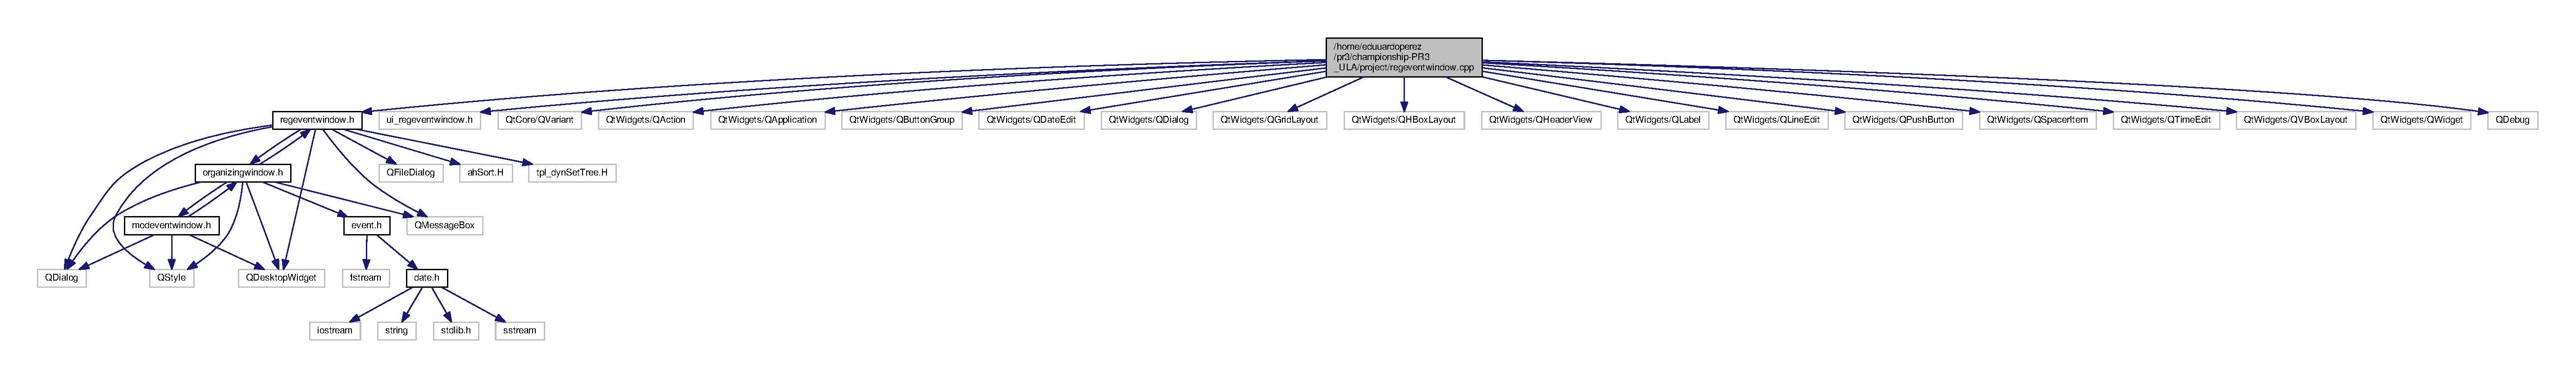
\includegraphics[width=350pt]{regeventwindow_8cpp__incl}
\end{center}
\end{figure}


\subsection{Descripción detallada}
Implementación de la clase \hyperlink{class_reg_event_window}{Reg\+Event\+Window}. 

\begin{DoxyAuthor}{Autor}
Eduardo Perez (\href{mailto:edujpp1@gmail.com}{\tt edujpp1@gmail.\+com}) 
\end{DoxyAuthor}
\begin{DoxyVersion}{Versión}
1.\+0 
\end{DoxyVersion}
\begin{DoxyDate}{Fecha}
Noviembre, 2016 
\end{DoxyDate}

\hypertarget{regeventwindow_8h}{}\section{Referencia del Archivo /home/eduuardoperez/pr3/championship-\/\+P\+R3\+\_\+\+U\+L\+A/project/regeventwindow.h}
\label{regeventwindow_8h}\index{/home/eduuardoperez/pr3/championship-\/\+P\+R3\+\_\+\+U\+L\+A/project/regeventwindow.\+h@{/home/eduuardoperez/pr3/championship-\/\+P\+R3\+\_\+\+U\+L\+A/project/regeventwindow.\+h}}


Clase \hyperlink{class_reg_event_window}{Reg\+Event\+Window}.  


{\ttfamily \#include $<$Q\+Dialog$>$}\\*
{\ttfamily \#include $<$Q\+Style$>$}\\*
{\ttfamily \#include $<$Q\+Desktop\+Widget$>$}\\*
{\ttfamily \#include $<$Q\+Message\+Box$>$}\\*
{\ttfamily \#include $<$Q\+File\+Dialog$>$}\\*
{\ttfamily \#include $<$ah\+Sort.\+H$>$}\\*
{\ttfamily \#include $<$tpl\+\_\+dyn\+Set\+Tree.\+H$>$}\\*
{\ttfamily \#include \char`\"{}organizingwindow.\+h\char`\"{}}\\*
Dependencia gráfica adjunta para regeventwindow.\+h\+:\nopagebreak
\begin{figure}[H]
\begin{center}
\leavevmode
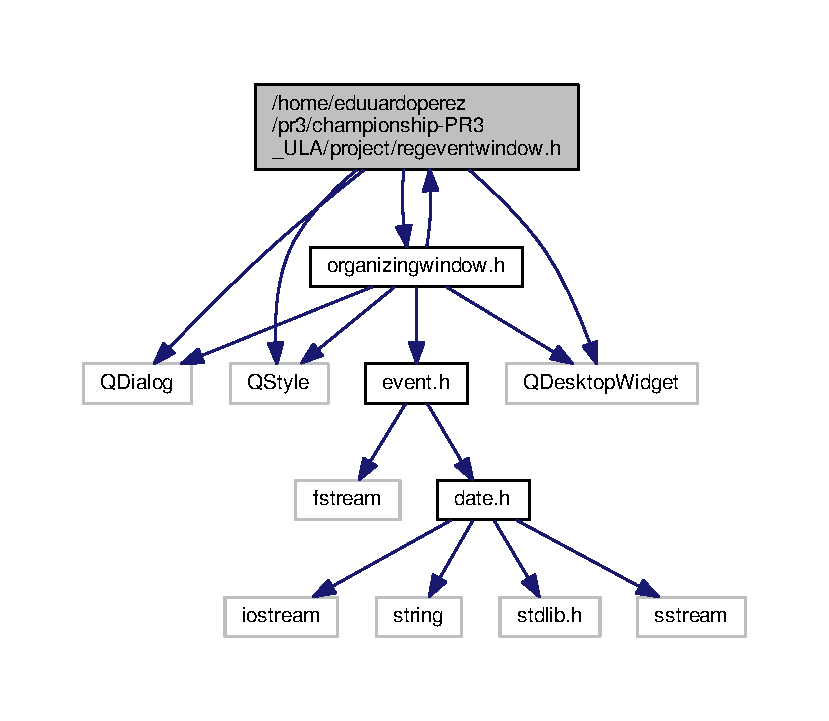
\includegraphics[width=350pt]{regeventwindow_8h__incl}
\end{center}
\end{figure}
Gráfico de los archivos que directa o indirectamente incluyen a este archivo\+:\nopagebreak
\begin{figure}[H]
\begin{center}
\leavevmode
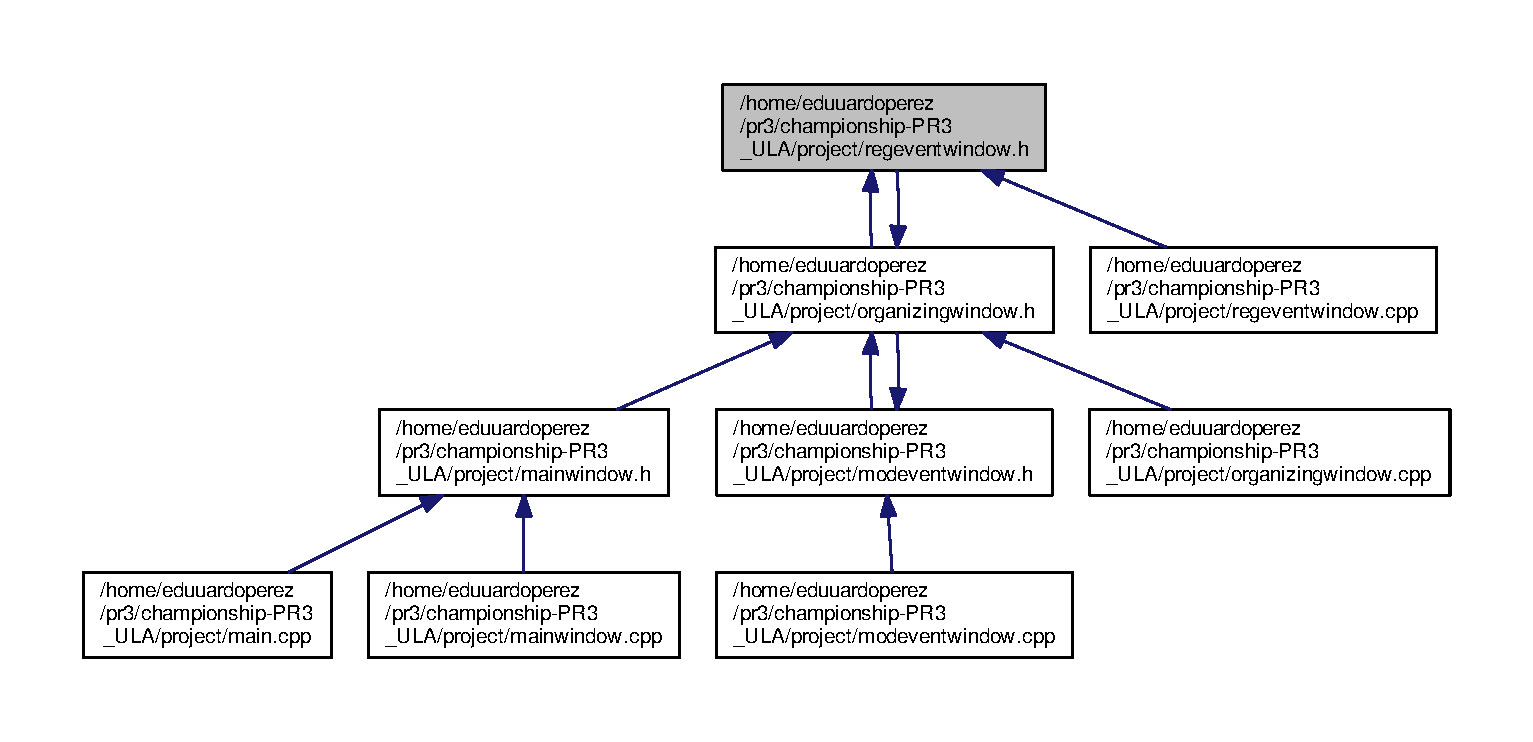
\includegraphics[width=350pt]{regeventwindow_8h__dep__incl}
\end{center}
\end{figure}
\subsection*{Estructuras de datos}
\begin{DoxyCompactItemize}
\item 
class \hyperlink{class_reg_event_window}{Reg\+Event\+Window}
\begin{DoxyCompactList}\small\item\em Clase \hyperlink{class_reg_event_window}{Reg\+Event\+Window}. \end{DoxyCompactList}\end{DoxyCompactItemize}


\subsection{Descripción detallada}
Clase \hyperlink{class_reg_event_window}{Reg\+Event\+Window}. 

\begin{DoxyAuthor}{Autor}
Eduardo Perez (\href{mailto:edujpp1@gmail.com}{\tt edujpp1@gmail.\+com}) 
\end{DoxyAuthor}
\begin{DoxyVersion}{Versión}
1.\+0 
\end{DoxyVersion}
\begin{DoxyDate}{Fecha}
Noviembre, 2016 
\end{DoxyDate}

\hypertarget{sportywindow_8cpp}{}\section{Referencia del Archivo /home/eduuardoperez/pr3/championship-\/\+P\+R3\+\_\+\+U\+L\+A/project/sportywindow.cpp}
\label{sportywindow_8cpp}\index{/home/eduuardoperez/pr3/championship-\/\+P\+R3\+\_\+\+U\+L\+A/project/sportywindow.\+cpp@{/home/eduuardoperez/pr3/championship-\/\+P\+R3\+\_\+\+U\+L\+A/project/sportywindow.\+cpp}}


Implementación de la clase \hyperlink{class_sporty_window}{Sporty\+Window}.  


{\ttfamily \#include \char`\"{}sportywindow.\+h\char`\"{}}\\*
{\ttfamily \#include \char`\"{}ui\+\_\+sportywindow.\+h\char`\"{}}\\*
Dependencia gráfica adjunta para sportywindow.\+cpp\+:\nopagebreak
\begin{figure}[H]
\begin{center}
\leavevmode
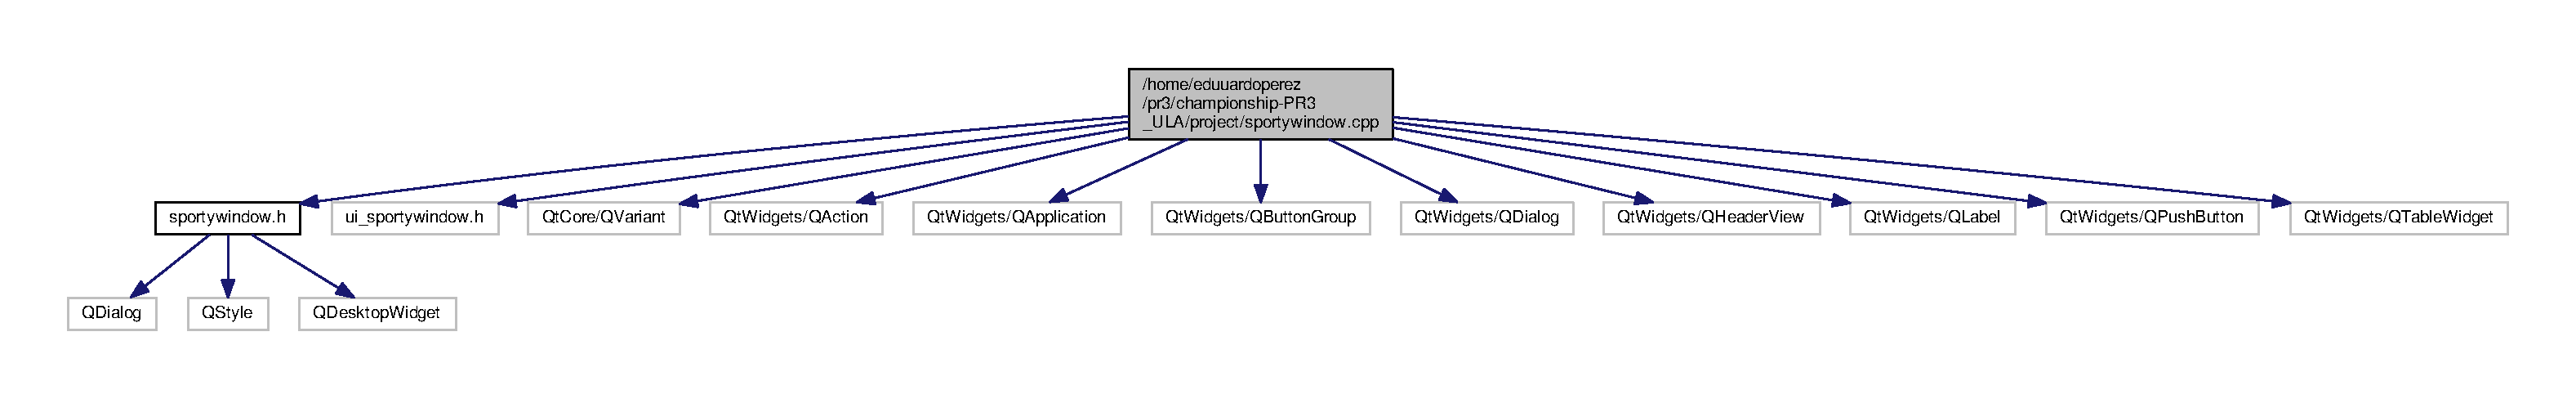
\includegraphics[width=350pt]{sportywindow_8cpp__incl}
\end{center}
\end{figure}


\subsection{Descripción detallada}
Implementación de la clase \hyperlink{class_sporty_window}{Sporty\+Window}. 

\begin{DoxyAuthor}{Autor}
Eduardo Perez (\href{mailto:edujpp1@gmail.com}{\tt edujpp1@gmail.\+com}) 
\end{DoxyAuthor}
\begin{DoxyVersion}{Versión}
1.\+0 
\end{DoxyVersion}
\begin{DoxyDate}{Fecha}
Noviembre, 2016 
\end{DoxyDate}

\hypertarget{sportywindow_8h}{}\section{Referencia del Archivo /home/eduuardoperez/pr3/championship-\/\+P\+R3\+\_\+\+U\+L\+A/project/sportywindow.h}
\label{sportywindow_8h}\index{/home/eduuardoperez/pr3/championship-\/\+P\+R3\+\_\+\+U\+L\+A/project/sportywindow.\+h@{/home/eduuardoperez/pr3/championship-\/\+P\+R3\+\_\+\+U\+L\+A/project/sportywindow.\+h}}


Clase \hyperlink{class_sporty_window}{Sporty\+Window}.  


{\ttfamily \#include $<$Q\+Dialog$>$}\\*
{\ttfamily \#include $<$Q\+Style$>$}\\*
{\ttfamily \#include $<$Q\+Desktop\+Widget$>$}\\*
Dependencia gráfica adjunta para sportywindow.\+h\+:\nopagebreak
\begin{figure}[H]
\begin{center}
\leavevmode
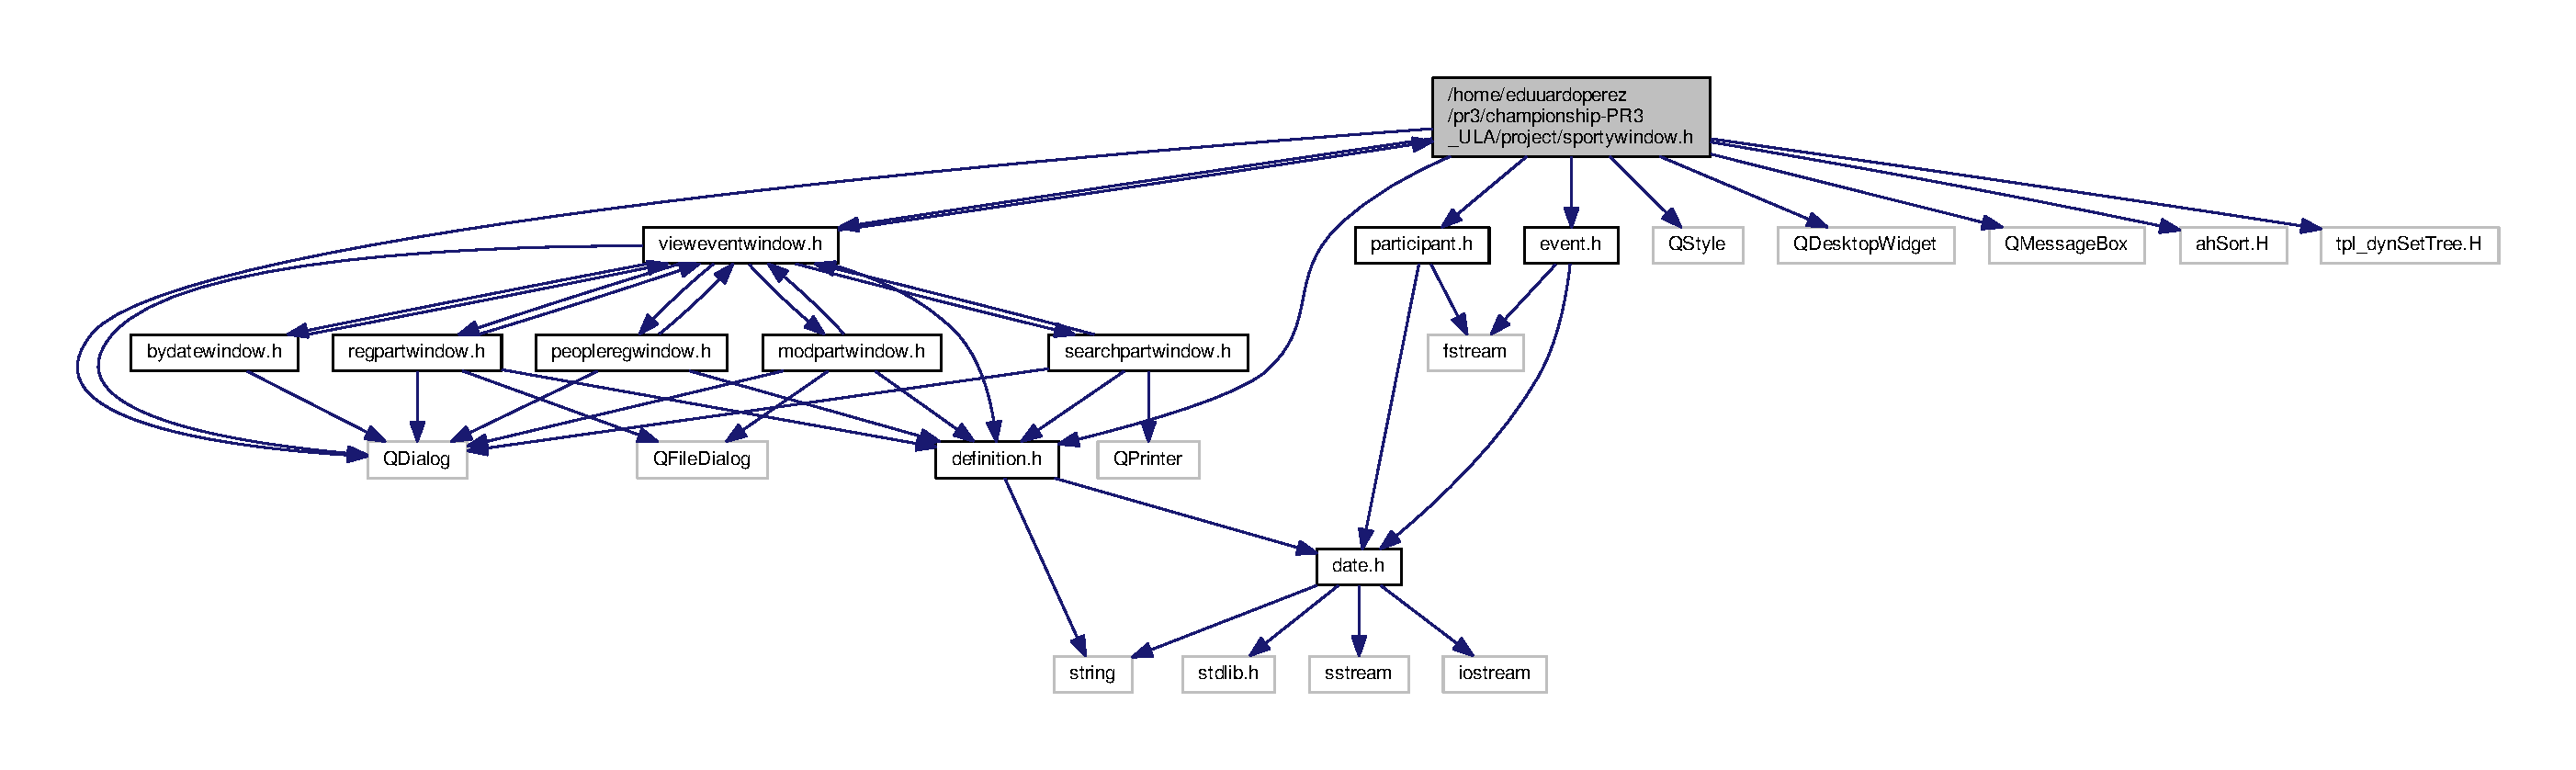
\includegraphics[width=308pt]{sportywindow_8h__incl}
\end{center}
\end{figure}
Gráfico de los archivos que directa o indirectamente incluyen a este archivo\+:\nopagebreak
\begin{figure}[H]
\begin{center}
\leavevmode
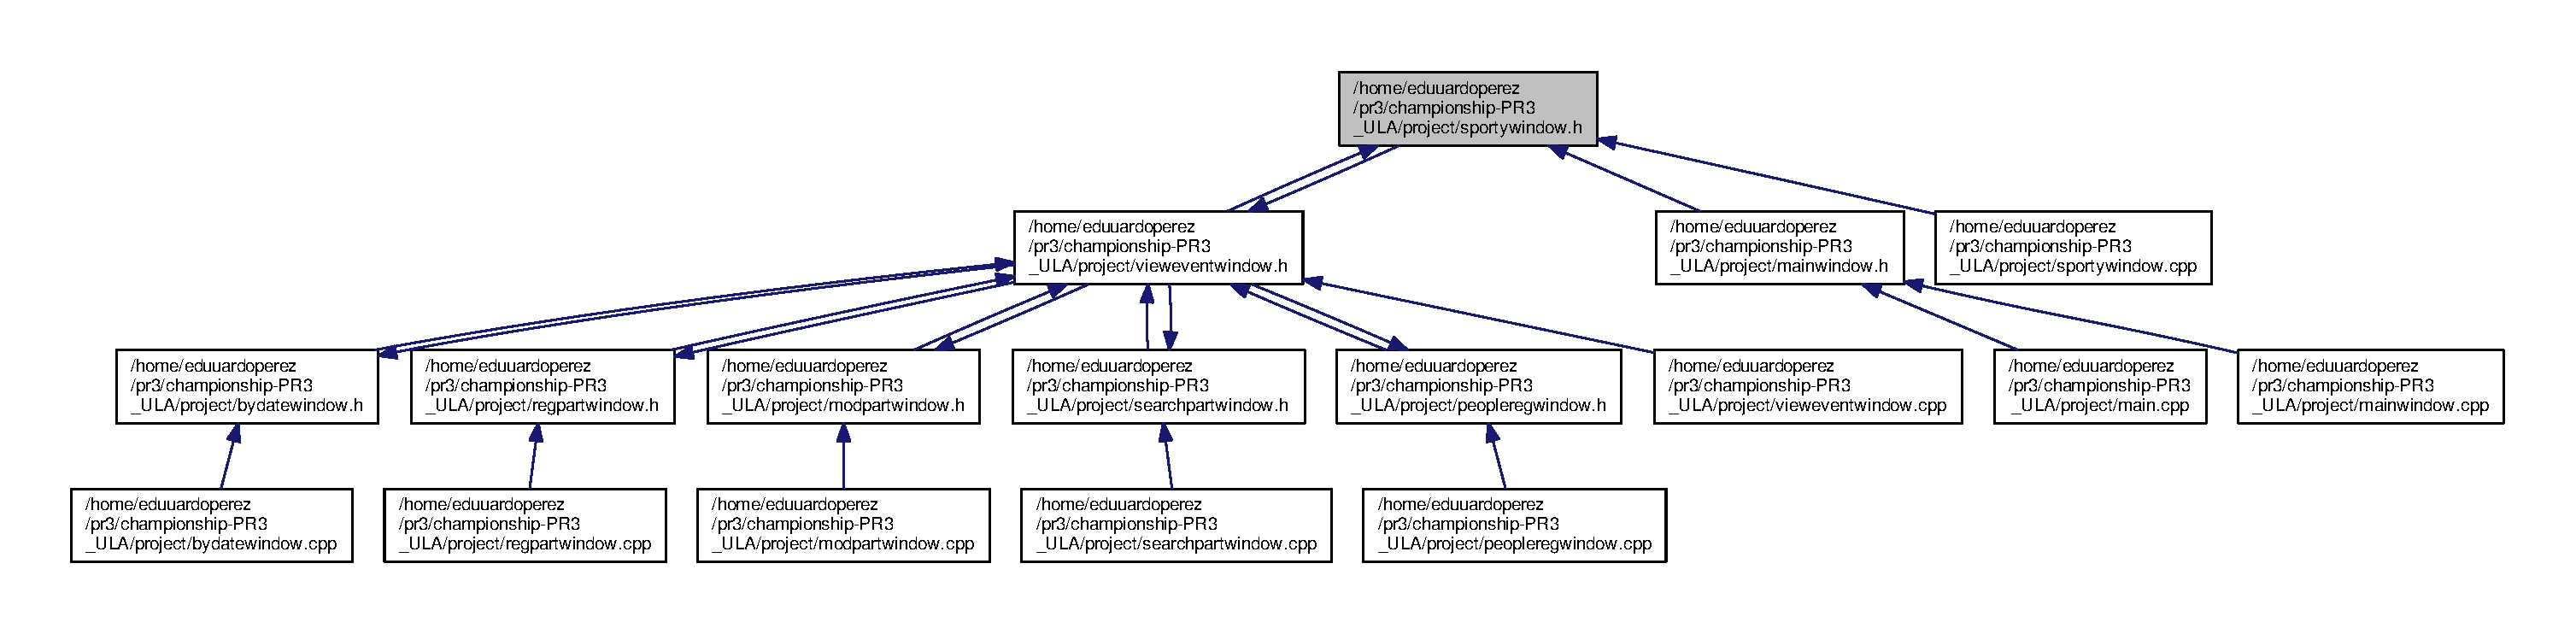
\includegraphics[width=350pt]{sportywindow_8h__dep__incl}
\end{center}
\end{figure}
\subsection*{Estructuras de datos}
\begin{DoxyCompactItemize}
\item 
class \hyperlink{class_sporty_window}{Sporty\+Window}
\begin{DoxyCompactList}\small\item\em Clase \hyperlink{class_sporty_window}{Sporty\+Window}. \end{DoxyCompactList}\end{DoxyCompactItemize}


\subsection{Descripción detallada}
Clase \hyperlink{class_sporty_window}{Sporty\+Window}. 

\begin{DoxyAuthor}{Autor}
Eduardo Perez (\href{mailto:edujpp1@gmail.com}{\tt edujpp1@gmail.\+com}) 
\end{DoxyAuthor}
\begin{DoxyVersion}{Versión}
1.\+0 
\end{DoxyVersion}
\begin{DoxyDate}{Fecha}
Noviembre, 2016 
\end{DoxyDate}

%--- End generated contents ---

% Index
\backmatter
\newpage
\phantomsection
\clearemptydoublepage
\addcontentsline{toc}{chapter}{Índice}
\printindex

\end{document}
